% This LaTeX document needs to be compiled with XeLaTeX.
\documentclass[10pt]{article}
\usepackage[utf8]{inputenc}
\usepackage{ucharclasses}
\usepackage{amsmath}
\usepackage{amsfonts}
\usepackage{amssymb}
\usepackage[version=4]{mhchem}
\usepackage{extpfeil}
\usepackage{stmaryrd}
\usepackage{bbold}
\usepackage{graphicx}
\usepackage[export]{adjustbox}
\graphicspath{ {./images/} }
\usepackage{caption}
\usepackage{hyperref}
\hypersetup{colorlinks=true, linkcolor=blue, filecolor=magenta, urlcolor=cyan,}
\urlstyle{same}
\usepackage[fallback]{xeCJK}
\usepackage{polyglossia}
\usepackage{fontspec}
\IfFontExistsTF{Noto Serif CJK TC}
{\setCJKmainfont{Noto Serif CJK TC}}
{\IfFontExistsTF{STSong}
  {\setCJKmainfont{STSong}}
  {\IfFontExistsTF{Droid Sans Fallback}
    {\setCJKmainfont{Droid Sans Fallback}}
    {\setCJKmainfont{SimSun}}
}}

\setmainlanguage{vietnamese}
\setotherlanguages{english}
\newfontfamily\vietnamesefont{CMU Serif}
\IfFontExistsTF{CMU Serif}
{\newfontfamily\lgcfont{CMU Serif}}
{\IfFontExistsTF{DejaVu Sans}
  {\newfontfamily\lgcfont{DejaVu Sans}}
  {\newfontfamily\lgcfont{Georgia}}
}
\setDefaultTransitions{\lgcfont}{}
\setTransitionsFor{Vietnamese}{\vietnamesefont}{\lgcfont}

%New command to display footnote whose markers will always be hidden
\let\svthefootnote\thefootnote
\newcommand\blfootnotetext[1]{%
  \let\thefootnote\relax\footnote{#1}%
  \addtocounter{footnote}{-1}%
  \let\thefootnote\svthefootnote%
}

%Overriding the \footnotetext command to hide the marker if its value is `0`
\let\svfootnotetext\footnotetext
\renewcommand\footnotetext[2][?]{%
  \if\relax#1\relax%
    \ifnum\value{footnote}=0\blfootnotetext{#2}\else\svfootnotetext{#2}\fi%
  \else%
    \if?#1\ifnum\value{footnote}=0\blfootnotetext{#2}\else\svfootnotetext{#2}\fi%
    \else\svfootnotetext[#1]{#2}\fi%
  \fi
}

\begin{document}
\captionsetup{singlelinecheck=false}
\section*{CÂU HỎI VÀ BÀI TẬP}
\section*{CHỦDỀ 1 ; ESTER = LIPID}
\section*{DRI \\
 1 ESTER - LIPID}
1.1. Điền các từ hoặc cụm từ trong khung vào chỗ trống của các phát biểu sau cho phù hợp.

Khōng phān cuc, nuơc, khong phān nhánh, -COOH, triglyceride, phân cuc, chăn, COO-, OH, monocarboxylic acid, triester, té bado sóng, glycerol, \_OR\\
a) Khi thay thế nhóm ... (1)... ở nhóm ... (2)... của carboxylic acid bằng nhóm ... (3) ... thì thu được ester.\\
b) Lipid là các hợp chất hữu cơ có trong ...(4)..., không tan trong ...(5)... nhưng tan được trong các dung môi hữu cơ ...(6)....\\
c) Chất béo là ...(7)... của acid béo và ... (8)..., chất béo còn được gọi chung là ...(9)....\\
d) Acid béo tạo nên chất béo thường là các ...(10)... có mạch carbon ...(11) ... và có số nguyên tử carbon ...(12) ...\\
1.2. Chất nào sau đây thuộc loại ester?\\
A. $\mathrm{CH}_{3} \mathrm{OOCC}_{2} \mathrm{H}_{5}$.\\
B. $\mathrm{HOOCCH}_{3}$.\\
C. $\mathrm{H}_{2} \mathrm{NCH}_{2} \mathrm{COOH}$.\\
D. $\mathrm{CH}_{3} \mathrm{CHO}$.\\
1.3. Cho các chất có công thức sau: $\mathrm{HCHO}, \mathrm{C}_{2} \mathrm{H}_{2}, \mathrm{CH}_{3} \mathrm{COOH}, \mathrm{CH}_{3} \mathrm{COOCH}=\mathrm{CH}_{2}$, $\mathrm{HCOOCH}_{3}, \mathrm{HCOOH}$. Trong các chất trên, có bao nhiêu chất thuộc loại ester?\\
A. 2 .\\
B. 3 .\\
C. 4 .\\
D. 5 .\\
1.4. Ester X mạch hở có công thức phân tử $\mathrm{C}_{3} \mathrm{H}_{4} \mathrm{O}_{2}$. Tên gọi của X là\\
A. vinyl acetate.\\
B. methyl acetate.\\
C. methyl formate.\\
D. vinyl formate.\\
1.5. Ester được tạo thành từ $\mathrm{CH}_{3} \mathrm{COOH}$ và $\mathrm{C}_{2} \mathrm{H}_{5} \mathrm{OH}$ có công thức cấu tạo là\\
A. $\mathrm{CH}_{3} \mathrm{COOCH}_{3}$.\\
B. $\mathrm{CH}_{3} \mathrm{COOC}_{2} \mathrm{H}_{5}$.\\
C. $\mathrm{C}_{2} \mathrm{H}_{5} \mathrm{COOCH}_{3}$.\\
D. $\mathrm{HCOOC}_{2} \mathrm{H}_{5}$.\\
1.6. Ester có công thức phân tử là $\mathrm{C}_{2} \mathrm{H}_{4} \mathrm{O}_{2}$ được tạo thành từ methyl alcohol và carboxylic acid nào sau đây?\\
A. Propionic acid.\\
B. Acetic acid.\\
C. Formic acid.\\
D. Oxalic acid.\\
1.7. Một hợp chất hữu cơ $\mathbb{X}$ đơn chức có công thức phân tử là $\mathrm{C}_{3} \mathrm{H}_{6} \mathrm{O}_{2} \cdot \mathbb{X}$ không tác dụng với kim loại Na nhung tác dụng được với dung dịch NaOH khi đun nóng. Chất X thuộc dãy đồng đẳng của loại hợp chất nào sau đây?\\
A. Alcohol.\\
B. Ester.\\
C. Aldehyde.\\
D. Carboxylic acid.\\
1.8. Trường hợp nào sau đây xảy ra phản ứng với ethyl acetate?\\
A. Dung dịch $\mathrm{NaOH}\left(\mathrm{t}^{\circ}\right)$.\\
B. $\mathrm{C}_{2} \mathrm{H}_{5} \mathrm{OH}$.\\
C. Dung dịch $\left[\mathrm{Ag}\left(\mathrm{NH}_{3}\right)_{2}\right] \mathrm{OH}$.\\
D. Dung dich NaCl .\\
1.9. Thuỷ phân ester $\mathbb{E}$ có công thức phân tử $\mathrm{C}_{4} \mathrm{H}_{8} \mathrm{O}_{2}$ với xúc tác acid vô cơ loãng, thu được hai sản phẩm hữu cơ $\mathrm{X}, \mathrm{Y}$ (chỉ chứa các nguyên tử $\mathrm{C}, \mathrm{H}, \mathrm{O}$ ). Từ $X$ có thể điều chế trực tiếp ra $Y$ bằng một phản ứng duy nhất. Chất $X$ là chất nào sau đây?\\
A. Acetic acid.\\
B. Ethyl alcohol.\\
C. Ethyl acetate.\\
D. Formic acid.\\
1.10. Cho các phản ứng sau:\\
(1) Thuỷ phân ester trong môi trường acid.\\
(2) Thuỷ phân ester trong dung dịch NaOH , đun nóng.\\
(3) Cho ester tác dụng với dung dịch KOH , đun nóng.\\
(4) Thuỷ phân dẫn xuất halogen trong dung dịch NaOH , đun nóng.\\
(5) Cho carboxylic acid tác dụng với dung dịch NaOH .

Những phản ứng nào không được gọi là phản ứng xà phòng hoá?\\
A. (1), (2), (3), (4).\\
B. (1), (4), (5).\\
C. (1), (3), (4), (5).\\
D. (3), (4), (5).\\
1.11. Phát biểu nào sau đây là kinông đúng?\\
A. So với các đồng phân là carboxylic acid, ester luôn có nhiệt độ sôi thấp hơn.\\
B. Phản ứng ester hoá là phản ứng thuận nghịch.\\
C. Phản ứng xà phòng hoá là phản ứng thuận nghịch.\\
D. Ester là những chất lỏng hoặc chất rắn ở nhiệt độ thường.\\
1.12. Tiến hành thí nghiệm điều chế isoamyl acetate (chất có mùi chuối chín) theo thứ tự các bước sau đây:\\
Buớc 1: Cho khoảng $3 \mathrm{~mL} \mathrm{CH} 3 \mathrm{CH}\left(\mathrm{CH}_{3}\right) \mathrm{CH}_{2} \mathrm{CH}_{2} \mathrm{OH}, 3 \mathrm{~mL} \mathrm{CH}_{3} \mathrm{COOH}$ và vài giọt $\mathrm{H}_{2} \mathrm{SO}_{4}$ đặc vào ống nghiệm.\\
Bước 2: Lắc đều ống nghiệm rồi đun cách thuỷ (trong nồi nước nóng) khoảng $5-7$ phút ở $65-70^{\circ} \mathrm{C}$.\\
Buóc 3: Làm lạnh, sau đó thêm khoảng 5 mL dung dịch NaCl bão hoà vào ống nghiệm.\\
Những phát biểu nào sau đây là đúng?\\
(a) $\mathrm{H}_{2} \mathrm{SO}_{4}$ đặc có vai trò xúc tác cho phản ứng tạo isoamyl acetate.\\
(b) Thêm dung dịch NaCl bão hoà vào để tránh phân huỷ sản phẩm.\\
(c) Sau bước 2, trong ống nghiệm vẫn còn $\mathrm{CH}_{3} \mathrm{CH}\left(\mathrm{CH}_{3}\right) \mathrm{CH}_{2} \mathrm{CH}_{2} \mathrm{OH}$ và $\mathrm{CH}_{3} \mathrm{COOH}$.\\
(d) Sau bước 3, trong ống nghiệm thu được hỗn hợp chất lỏng đồng nhất.\\
1.13. Quan sát hình sau.

\begin{figure}[h]
\begin{center}
  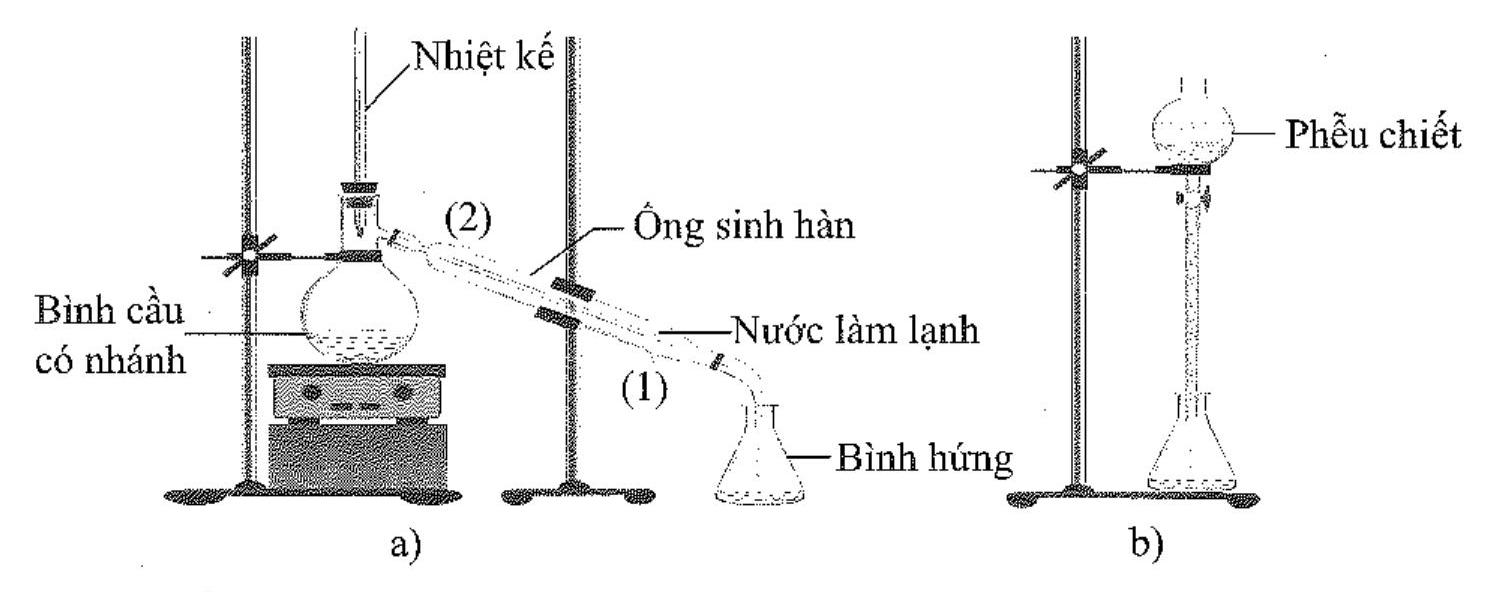
\includegraphics[width=\textwidth]{2025_10_23_80c1361fcdcd395cad8eg-03}
\captionsetup{labelformat=empty}
\caption{Hình 1.i. Minh hoạ phương pháp điều chế isoamyl acetate trong phòng thí nghiệm}
\end{center}
\end{figure}

Cho các phát biểu liên quan tới Hình 1.1 như sau:\\
(1) Hỗn hợp chất lỏng trưởc phản ứng trong bình cầu có nhánh gồm isoamyl alcohol, acetic acid và sulfuric acid đặc.\\
(2) Trong phễu chiết, lớp chất lỏng nặng hơn có thành phần chính là isoamyl acetate.\\
(3) Nhiệt kế đùng để kiểm soát nhiệt độ trong bình cầu có nhánh.\\
(4) Phễu chiết dùng để tách isoamyl acetate ra khỏi hỗn hợp sau phản ứng.\\
(5) Nước làm lạnh cho chảy vào ống sinh hàn ở vị trí (1) và chảy ra ở vị trí (2). Số phát biểu đúng là\\
A. 3 .\\
B. 2 .\\
C. 4 .\\
D. 5 .\\
1.14. Ester là một loại hợp chất hữu cơ phổ biến và có vai trò quan trọng trong lĩnh vực hoá học và công nghiệp như làm dung môi, chất tạo hương, nguyên liệu tổng hợp polymer,... Các ester chủ yếu được điều chế từ phản ứng ester hoá. Những phát biểu nào sau đây là đúng?\\
(a) Methyl formate là ester có phân tử khối nhỏ nhất.\\
(b) Ethyl acetate là ester tan tốt trong nước.\\
(c) Trong phân tử ester no, đơn chức, mạch hở có chứa một liên kết $\pi$.\\
(d) Benzyl acetate có công thức phân tử $\mathrm{C}_{9} \mathrm{H}_{10} \mathrm{O}_{2}$.\\
(e) Ester là sản phẩm của phản ứng giữa acid và alcohol.\\
(g) Ester là hợp chất hữu cơ trong phân tử có nhóm $-\mathrm{COO}-$.\\
(h) Ester no, đơn chức, mạch hở có công thức phân tử $\mathrm{C}_{\mathrm{n}} \mathrm{H}_{2 \mathrm{n}} \mathrm{O}_{2}(\mathrm{n} \geq 2)$.\\
(i) Hợp chất $\mathrm{CH}_{3} \mathrm{OOCC}_{2} \mathrm{H}_{5}$ thuộc dãy đồng đẳng của methyl formate.\\
1.15. Để xà phòng hoá hoàn toàn $2,64 \mathrm{~g}$ một ester no, đơn chức, mạch hở X cần dùng $30,0 \mathrm{~mL}$ dung dịch $\mathrm{NaOH} 1,0 \mathrm{M}$. Công thức phân tử của ester X là\\
A. $\mathrm{C}_{3} \mathrm{H}_{6} \mathrm{O}_{2}$.\\
B. $\mathrm{C}_{4} \mathrm{H}_{8} \mathrm{O}_{2}$.\\
C. $\mathrm{C}_{5} \mathrm{H}_{10} \mathrm{O}_{2}$.\\
D. $\mathrm{C}_{6} \mathrm{H}_{10} \mathrm{O}_{2}$.\\
1.16. Kết quả phân tích nguyên tố của ester đơn chức X cho thấy X có $\% \mathrm{C}=60 \%$, $\% \mathrm{H}=8 \%$ (về khối lượng), còn lại là O . Trên phổ MS của X thấy xuất hiện tín hiệu của ion phân tử $\left[\mathrm{M}^{+}\right]$có giá trị $m / z=100$. Biết $\mathbb{X}$ được tạo bởi từ phản ứng ester hoá giữa alcohol mạch không nhánh với carboxylic acid mạch phân nhánh. Dự đoán công thức cấu tạo và tên gọi của X .\\
1.17. Để điều chế isoamyl acetate trong phòng thí nghiệm, một học sinh đã đun nóng $4,00 \mathrm{~mL}$ acetic acid ( $\mathrm{D}=1,05 \mathrm{~g} \mathrm{~mL}^{-1}$ ) với $8,00 \mathrm{~mL}$ isoamyl alcohol $\left(\mathrm{CH}_{3}\right)_{2} \mathrm{CHCH}_{2} \mathrm{CH}_{2} \mathrm{OH}\left(\mathrm{D}=0,81 \mathrm{~g} \mathrm{~mL}{ }^{-1}\right)$, có dung dịch $\mathrm{H}_{2} \mathrm{SO}_{4}$ đặc làm xúc tác, thu được $6,00 \mathrm{~mL}$ isoamyl acetate ( $\mathrm{D}=0,88 \mathrm{~g} \mathrm{~mL}^{-1}$ ). Tính hiệu suất của phản ứng.\\
1.18. Hợp chất hữu cơ đơn chức X ở điều kiện thường là chất lỏng, có mùi thơm, được ứng dụng làm dung môi, chất tạo hương,... Kết quả phân tích nguyên tố cho thấy X có thành phần phần trăm về khối lượng của C và H lần lượt là $48,65 \%$ và $8,11 \%$, còn lại là O . Trên phổ MS của X thấy xuất hiện tín hiệu của ion phân tử $\left[\mathrm{M}^{+}\right]$có giá trị $m / z=74$. Trên phổ $\mathbb{R}$ của $X$ thấy có tín hiệu đặc trưng ở vùng $1750-1715 \mathrm{~cm}^{-1}$.\\
a) Xác định công thức cấu tạo của X .\\
b) X thường được tổng hợp bằng cách đun nóng hỗn hợp gồm chất hữu cơ $\mathbb{A}$ và chất hữu cơ $\mathbb{B}$, có dung dịch $\mathrm{H}_{2} \mathrm{SO}_{4}$ đặc làm xúc tác. Xác định công thức cấu tạo của $\mathbb{A}$ và $\mathbb{B}$. Viết phương trình hoá học điều chế $\mathbb{X}$ từ $\mathbb{A}$ và $\mathbb{B}$.

\section*{Bai \\
 2 XÀ PHÒNG VÀ CHẤT GIẶT RỦA TỔNG HỢP}
2.1. Điền các từ hoặc cụm từ cho trong khung vào chỗ trống của mỗi phát biểu sau cho phù hợp.

\section*{chát béo, ua nuóc, li nuóc, acid béo, triglyceride, potassium, dâu mó, giāt ría, muót}
a) Xà phòng là hỗn hợp muối sodium hoặc ...(1)... của ...(2)... và một số chất phụ gia.\\
b) Chất giặt rưa có thành phần không phải muối của ...(3)..., nhưng có tính chất ... (4)... như xà phòng.\\
c) Chất giặt rửa tổng hợp được sản xuất chủ yếu từ nguyên liệu ... (5) ... Xà phòng được sản xuất từ ...(6)... hoặc từ ...(7)....\\
2.2. Trong thực tế, người ta dùng phản ửng nào sau đây để điều chế xà phòng?\\
A. Đun nóng acid béo với dung dịch kiềm.\\
B. Đun nóng chất béo với dung dịch kiềm.\\
C. Đun nóng glycerol với các acid béo.\\
D. Đun nóng acid béo hoặc chất béo với dung dịch kiềm.\\
2.3. Khi xà phòng hoá tristearin thu được sản phẩm là\\
A. $\mathrm{C}_{15} \mathrm{H}_{31} \mathrm{COONa}$ và $\mathrm{C}_{2} \mathrm{H}_{5} \mathrm{OH}$.\\
B. $\mathrm{C}_{17} \mathrm{H}_{35} \mathrm{COOH}$ và $\mathrm{C}_{3} \mathrm{H}_{5}(\mathrm{OH})_{3}$.\\
C. $\mathrm{C}_{15} \mathrm{H}_{31} \mathrm{COOH}$ và $\mathrm{C}_{3} \mathrm{H}_{5}(\mathrm{OH})_{3}$.\\
D. $\mathrm{C}_{17} \mathrm{H}_{35} \mathrm{COONa}$ và $\mathrm{C}_{3} \mathrm{H}_{5}(\mathrm{OH})_{3}$.\\
2.4. Chất nào sau đây là thành phần chủ yếu của xà phòng?\\
A. $\mathrm{CH}_{3} \mathrm{COONa}$.\\
B. $\mathrm{CH}_{3}\left(\mathrm{CH}_{2}\right)_{3} \mathrm{COONa}$.\\
C. $\mathrm{CH}_{2}=\mathrm{CHCOONa}$.\\
D. $\mathrm{C}_{17} \mathrm{H}_{35} \mathrm{COONa}$.\\
2.5. Từ tristearin, người ta dùng phản ứng nào để điều chế xà phòng?\\
A. Phản ứng ester hoá.\\
B. Phản ứng thuỷ phân ester trong môi trường acid.\\
C. Phản ứng công hydrogen.\\
D. Phản ứng thuỷ phân ester trong môi trường kiềm.\\
2.6 Chất nào sau đây là thành phần chính của chất giặt rửa tổng hợp?\\
A. $\mathrm{C}_{15} \mathrm{H}_{31} \mathrm{COONa}$.\\
B. $\left(\mathrm{C}_{17} \mathrm{H}_{35} \mathrm{COO}\right)_{2} \mathrm{Ca}$.\\
C.\\
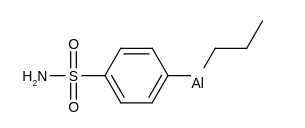
\includegraphics{smile-49f9c07844d7f9ccf075d51fbd261f56148542f2}\\
D. $\mathrm{C}_{17} \mathrm{H}_{35} \mathrm{COOK}$.\\
2.7. Những phát biểu nào sau đây là đúng?\\
(a) Xà phòng là sản phẩm của phản ứng xà phòng hoá.\\
(b) Muối sodium hoặc potassium của acid hữu cơ là thành phần chính của xà phòng.\\
(c) Khi đun nóng chất béo với đung dịch NaOH hoặc KOH , thu được xà phòng.\\
(d) Có thể sản xuất được xà phòng từ các alkane mạch dài thu được từ chế biến dầu mỏ.\\
2.8. Những phát biểu nào sau đây là đúng?\\
(a) Các chất giặt rửa đều được sản xuất bằng cách đun nóng dầu, mỡ động vật, thực vật với dung dịch kiềm.\\
(b) Xà phòng là hỗn hợp muối sodium hoặc potassium của acid béo, không nên dùng xà phòng trong nước cứng vì tạo ra muối kết tủa.\\
(c) Chất giặt rửa tổng hợp không phải là muối sodium của carboxylic acid và không bị kết tủa trong nước cứng.\\
(d) Các chất giặt rửa đều có khả năng hoạt động bề mặt cao, có tác dụng làm giảm sức căng bề mặt chất bẩn, giúp vải sợi dễ thấm uớt.\\
(e) Chất giặt rửa thường được cấu tạo gồm hai phần, một phần ưa nước và một phần kị nước.\\
(g) Chất giặt rửa tổng hợp tương tự với xà phòng ở phần kị nước, còn phần ưa nước là các nhóm khác nhau.\\
(h) Chất giặt rửa làm giảm sức căng bề mặt của dung dịch và tăng tính thấm uớt của vật cần giặt rửa.\\
(i) Từ nguồn nguyên liệu dầu mỏ, có thể sản xuất được cả xà phòng và chất giặt rưa tổng hợp.\\
2.9. Nêu những ưu điểm và hạn chế của việc dùng xà phòng so với dùng chất giặt rưa tổng hợp.\\
2.10. Cho khoảng 3-4 gam mỡ lợn (ở dạng lỏng) vào cốc thuỷ tinh chụu nhiệt chứa một lượng dư dung dịch NaOH , thấy chất trong cốc tách thành hai lớp; đun sôi hỗn hợp, đồng thời khuấy đều một thời gian đến khi thu được chất lòng đồng nhất; để nguội hỗn hợp và thêm vào một ít muối ăn, khuấy cho tan hết, thấy hỗn hợp tách thành hai lớp: phía trên là chất rắn màu trắng, phía dưới là chất lỏng. Hãy giải thích hiện tượng thí nghiệm trên và viết phương trình hoá học của phản ứng xảy ra.\\
2.11. Một loại mỡ động vật có chứa $30 \%$ tristearin, $40 \%$ tripalmitin và $30 \%$ triolein (về khối lượng).\\
a) Viết phương trình hoá học của các phản ứng xảy ra với NaOH khi thực hiện phản ứng xà phòng hoá loại mỡ trên để sản xuất xà phòng.\\
b) Xà phòng hoá 1 tấn mỡ trên bằng dung dịch NaOH với hiệu suất $85 \%$. Lượng muối thu được dùng để sản xuất xà phòng. Biết loại xà phòng này có $72 \%$ khối lượng là muối của acid béo. Tính khối lượng xà phòng thu được.

\section*{CHỦDỀ 2 CARBOHYDRATE}
\section*{BAI GIÓI THIỆU 3 VỂ CARBOHYDRATE}
3.1. Chất nào dưới đây là một disaccharide?\\
A. Saccharose.\\
B. Glucose.\\
C. Cellulose.\\
D. Fructose.\\
3.2. Chất nào dưới đây là một polysaccharide?\\
A. Saccharose.\\
B. Maltose.\\
C. Cellulose.\\
D. Fructose.\\
3.3. Tinh bột là hợp chất thuộc loại\\
A. disaccharide.\\
B. monosaccharide.\\
C. polysaccharide.\\
D. triglyceride.\\
3.4. Điền từ hoăc cụm từ thích hợp trong khung vào chỗ trống trong mỗi phát biểu sau.\\
cellulose; saccharose; maltose; $\alpha-1,2-g$ lycoside; $\alpha-1,4$-glycoside; P-1, 4-glycoside; B-1, 2-glycoside\\
a) Bông là ...(1)... gần như tinh khiết. Phân tử ...(1)... gồm các đơn vị glucose liên kết với nhau bằng liên kết ... (2)... tạo thành mạch dài.\\
b) Trong tự nhiên, ... (3)... là loại đường có nhiều trong cây mía, củ cải đường,... Phân tử ... (3)... gồm một đơn vị glucose và một đơn vị fructose liên kết với nhau bằng liên kết ...(4)....\\
3.5. Tinh bột và cellulose là các polymer lần lượt tạo bỏi các mắt xích\\
A. $\alpha$-fructose và $\beta$-glucose.\\
B. $\beta$-fructose và $\beta$-glucose.\\
C. $\alpha$-glucose và $\beta$-glucose.\\
D. $\alpha$-glucose và $\beta$-fructose.\\
3.6. Công thức nào dưới đây mô tả đúng cấu tạo của fructose ở dạng mạch hở?\\
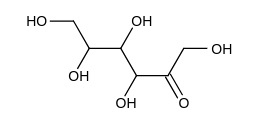
\includegraphics{smile-cbd802e308b52371710b858532258f8f3e5f00d4}

A.\\
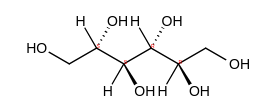
\includegraphics{smile-0efa660eba08f93ffd9514b836bfc9e10e8f2d29}

B.\\
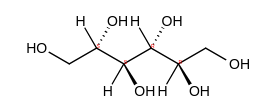
\includegraphics{smile-0dc4b4a8b08e126adc6943e268b83f9bb282cb13}

C.\\
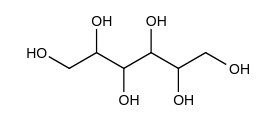
\includegraphics{smile-336260e74628460c0ad254fd104894bea57a1bb9}

D.\\
3.7. Carbohydrate nào sau đây kém tan trong nước lạnh nhưng tan được trong nước nóng tạo dung dịch keo, nhót?\\
A. Glucose.\\
B. Tinh bột.\\
C. Cellulose.\\
D. Saccharose.\\
3.8. Polymer là nguồn carbohydrate dự trữ có trong cơ thể động vật và được tạo thành từ các đơn vị glucose là\\
A. cellulose.\\
B. amylose.\\
C. amylopectin.\\
D. glycogen.\\
3.9. Polysaccharide mạch phân nhánh, có nhiều trong các loại ngũ cốc, thường được sứ dụng làm lương thực là\\
A. cellulose.\\
B. amylose.\\
C. amylopectin.\\
D. glycogen.\\
3.10. Chất có công thức phân tử $\mathrm{C}_{12} \mathrm{H}_{22} \mathrm{O}_{11}$, được tạo thành trong quá trình thuỷ phân không hoàn toàn amylose có trong tinh bột là\\
A. glucose.\\
B. saccharose.\\
C. fructose.\\
D. maltose.\\
3.11. Công thức nào dưới đây phù hợp với công thức cấu tạo của $\beta$-glucose?\\
A.\\
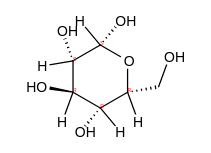
\includegraphics{smile-2403dbcd7d1a61a4bdaa5dd733569fd10be306e0}\\
B.\\
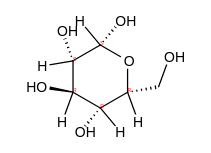
\includegraphics{smile-3798e02ee97051ea8743e970129d950e145b8a2a}\\
C.\\
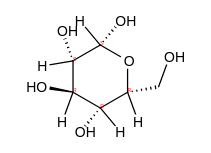
\includegraphics{smile-a6ca58fbedc49696409071369c30f728f230008a}\\
D.\\
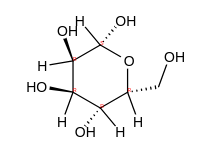
\includegraphics{smile-30b5312dcb266e6797c81b0ae8f1950700b64e16}\\
3.12. Trong công thức của fructose ở hình bên, nhóm -OH hemiketal là nhóm -OH được đánh số\\
A. 1 .\\
B. 3 .\\
C. 2.\\
D. 4 .\\
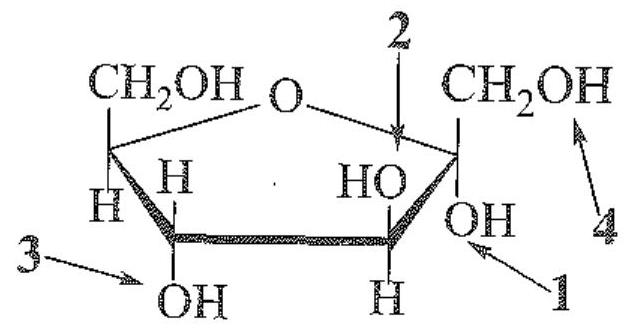
\includegraphics[max width=\textwidth, center]{2025_10_23_80c1361fcdcd395cad8eg-09}\\
3.13. Enzyme amylase chỉ có tác dụng thuỷ phân liên kết $\alpha$-glycoside giữa các đơn vị glucose. Chất nào dưới đây không chịu tác động của enzyme amylase?\\
A. Cellulose.\\
B. Amylose.\\
C. Amylopectin.\\
D. Glycogen.\\
3.14. Sorbitol $\left(\mathrm{C}_{6} \mathrm{H}_{14} \mathrm{O}_{6}\right)$ là một chất được dùng trong sản xuất một số loại bánh để tạo vị ngọt, đồng thời làm cho bánh giữ được độ ẩm, độ bóng mịn. Sorbitol cũng được dùng làm thuốc trị táo bón, khó tiêu. Sorbitol thường được tạo thành từ phản ứng hydrogen hoá glucose:\\
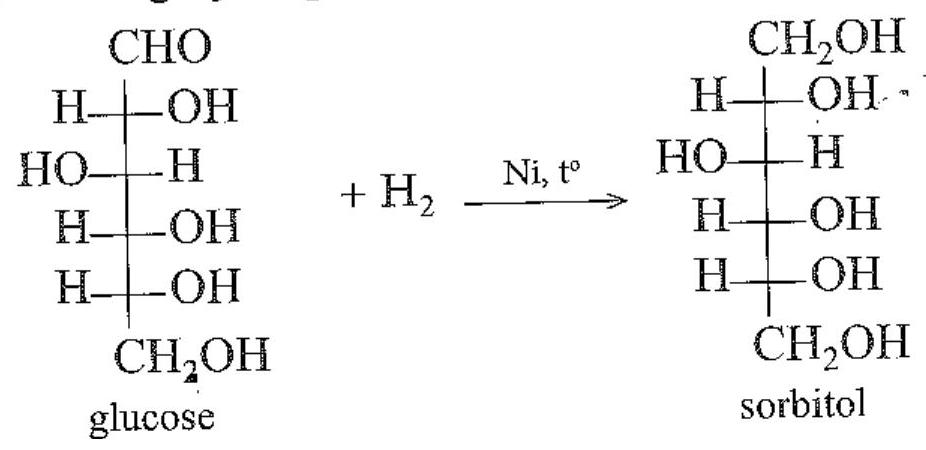
\includegraphics[max width=\textwidth, center]{2025_10_23_80c1361fcdcd395cad8eg-10}

Sorbito1 có thuộc loại hợp chất carbohydrate không? Vì sao?\\
3.15. Phổ hồng ngoại của fructose được cho ở Hình 3.1. Dựa vào những thông tin nào có thể kết luận: Trong điều kiện đo mẫu, fructose tồn tại chủ yếu ở dạng mạch vòng mà không phải ở dạng mạch hở?

\begin{figure}[h]
\begin{center}
  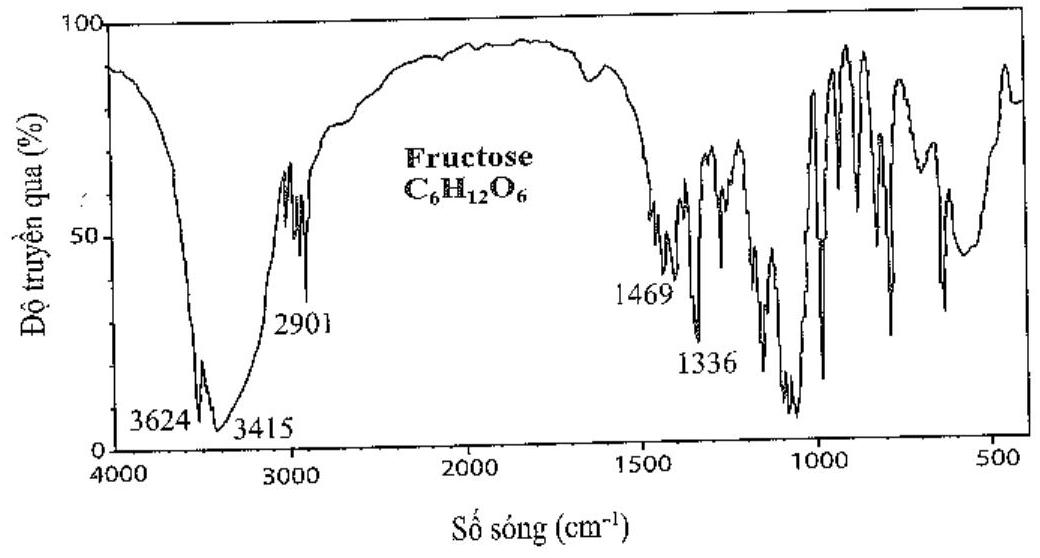
\includegraphics[width=\textwidth]{2025_10_23_80c1361fcdcd395cad8eg-10(1)}
\captionsetup{labelformat=empty}
\caption{Hình 3.1. Phồ hồng ngoại của fructose}
\end{center}
\end{figure}

3.16. Tìm hiểu và cho biết:\\
a) Ethanol sinh học là gì?\\
b) Ở nước ta hiện nay, ethanol sinh học được sản xuất từ nguyên liệu nào?

\section*{Bill 4. TÍNH CHẤT HOÁ HOC CỦA CARBOHYDRATE}
4.1. Điền các từ hoặc cụm từ trong khung vào chỗ trống của đoạn thông tin sau cho phù hợp.

\section*{do gach, xanh nhat, carbonyl, alcohol da chice, xanh lam, aldehyde, ketone, den}
Thêm từ từ 2 mL dung dịch $\mathrm{NaOH} 10 \%$ vào ống nghiệm chứa 1 mL dung dịch $\mathrm{CuSO}_{4} 5 \%$. Lắc đều ống nghiệm thấy xuất hiện kết tủa màu ... (1).... Tiếp tục thêm đừng giọt dung dịch glucose $2 \%$ vào ống nghiệm, lắc nhẹ. Kết tủa màu ... (1)... bị hoà tan và dung dịch có màu ... (2)..., chứng tỏ glucose có tính chất của ... (3).... Đun nóng ống nghiệm thấy tạo thành kết tủa đỏ gạch. Phản ứng xảy ra cho thấy glucose có tính chất của một ...(4)....\\
4.2. Monosaccharide $\mathbf{X}$ được dùng trong công nghiệp để tráng bạc lên bề mặt thuỷ tinh trong sản xuất ruột phích. Cùng với Ag , sản phẩm hữu cơ được tạo thành khi cho X tác dụng với lượng dư dung dịch $\mathrm{AgNO}_{3}$ trong $\mathrm{NH}_{3}$ là\\
A. ammonium carbonate.\\
B. ammonium gluconate.\\
C. gluconic acid.\\
D. khí carbon dioxide.\\
4.3. Có thể phân biệt glucose và fructose bằng cách cho từng chất tác dụng với\\
A. $\mathrm{Cu}(\mathrm{OH})_{2}$ trong môi trường kiềm, đun nóng.\\
B. thuốc thử Tollens.\\
C. dung dịch chứa $\mathrm{Cu}(\mathrm{OH})_{2}$.\\
D. nước bromine.\\
4.4. Mỗi phát biểu sau là đúng hay sai?\\
(a) Fructose có công thức phân tử là $\mathrm{C}_{6} \mathrm{H}_{10} \mathrm{O}_{5}$.\\
(b) Trong phân tử fructose có 5 nhóm -OH (alcohol) và một nhóm $>\mathrm{C}=\mathrm{O}$ (ketone).\\
(c) Fructose có khả năng tham gia phản ứng tráng bạc.\\
(d) Fructose được tạo thành trong phản ứng thuỷ phân tinh bột.\\
4.5. Cho hai chất M1 và M2 có công thức cấu tạo như sau:

M1:\\
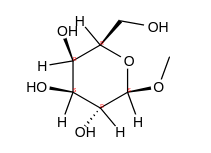
\includegraphics{smile-64bfddfaeb0c444e8179bb389e2f6fe9d4ab6373}

M2:\\
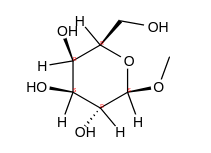
\includegraphics{smile-6192c6a20608b6969c02c99c33650295b6e878be}

Sản phẩm tạo thành khi dẫn khí hydrogen chloride vào dung dịch của glucose trong methanol\\
A. không là M1 hoặc M2.\\
B. chỉ là Mril.\\
C. chỉ là M2.\\
D. là hỗn hợp của M1 và M2.\\
4.6. Chất nào dưới đây kịnông có phản ứng tráng bạc khi cho phản ứng với thuốc thư Tollens?\\
A. Saccharose.\\
B. Glucose.\\
C. Maltose.\\
D. Fructose.\\
4.7. Dung dịch (1) chứa $\mathrm{CuSO}_{4}$ trong nước; dung dịch (2) là dung dịch ammonia có hoà tan một lượng $\mathrm{AgNO}_{3}$; dung dịch (3) là dung dịch ammonia có hoà tan một lượng $\mathrm{Cu}(\mathrm{OH})_{2}$. Dung dịch nào trong số các dung dịch trên có khả năng hoà tan cellulose?\\
A. Dung dịch (1).\\
B. Dung dịch (2).\\
C. Dung dịch (3).\\
D. Không dung dịch nào.\\
4.8. Saccharose là một disaccharide. Phát biểu nào sau đây về saccharose là đúng?\\
A. Saccharose không bị thuỷ phân trong môi trường acid.\\
B. Thuỷ phân saccharose chỉ thu được glucose.\\
C. Thuỷ phân saccharose thu được cả glucose và fructose.\\
D. Thuỷ phân saccharose chỉ thu được fructose.\\
4.9. Khi cho dung dịch saccharose vào ống nghiệm chứa $\mathrm{Cu}(\mathrm{OH})_{2} / \mathrm{NaOH}$, lắc nhẹ ống nghiệm thì thấy có biện tượng nào sau đây?\\
A. Kim loại màu vàng sáng bám trên bề mặt ống nghiệm.\\
B. Kết tủa màu đỏ gạch xuất hiện trong ống nghiệm.\\
C. Dưng dịch trở nên đồng nhất và có màu xanh lam.\\
D. Chất lỏng trong ống nghiệm tách thành hai lợp và xuất hiện kết tủa màu xanh nhạt lắng xuống đáy ống nghiệm.\\
4.10. Chất nào dưới đây không tan trong nước nhưng tan được trong dùng dịch Schweizer?\\
A. Saccharose.\\
B. Cellulose.\\
C. Maltose.\\
D. Fructose.\\
4.11. Khi tồn tại ở dạng mạch vòng, các carbohydrate có vị ngọt và có nhóm -OH hemiacetal hoặc -OH hemiketal trong phân tử được gọi là đường khử; ngược lại khi phân tử các chất này không có nhóm -OH hemiacetal hoặc -OH hemiketal, chúng được gọi là đường không có tính khử. Trong các đường saccharose, maltose, glucose, fructose, đường không có tính khử là\\
A. saccharose.\\
B. glucose.\\
C. maltose.\\
D. fructose.\\
4.12. Tinh bột không chỉ là chất dinh dưỡng quan trọng trong đời sống mà còn là nguyên liệu chủ yếu để sản xuất bánh, rượu, bia,... Nhận định nào sau đây về tính chất của tinh bột là không đúng?\\
A. Dung dịch hồ tinh bột tạo với iodine hợp chất màu xanh tím.\\
B. Tinh bột có khả năng tham gia phản ứng tráng bạc.\\
C. Tinh bột bị thuỷ phân trong môi trường acid cho sản phẩm cuối cùng là glucose.\\
D. Thuỷ phân hoàn toàn tinh bột bởi enzyme amylase cho sản phẩm là glucose.\\
4.13. Trong quá trình sản xuất bia bằng phương pháp lên men sinh học, dưới tác dưng của enzyme sẽ xảy ra quá trình chuyển hoá: $X \rightarrow$ maltose $\rightarrow Y$.\\
$\mathrm{X}, \mathrm{Y}$ tương ứng là\\
A. tinh bột và fructose.\\
B. cellulose và glucose.\\
C. cellulose và fructose.\\
D. tinh bột và glucose.\\
4.14. Khi đun nóng dung dịch chứa carbohydrate X và $\mathrm{Cu}(\mathrm{OH})_{2}$ trong môi truờng kiềm, X có phản ứng với $\mathrm{Cu}(\mathrm{OH})_{2}$ tạo kết tủa đỏ gạch. X khômg thể là\\
A. saccharose.\\
B. glucose.\\
C. fructose.\\
D. maltose.\\
4.15. Trong quá trình sản xuất rượu vang, người ta sử dụng nấm men Saccharomyces cerevisiae để lên men glucose và fructose (có trong dịch ép trái nho) tạo thành ethanol. Một học sinh thực hiện thí nghiệm thử tính chất của sản phẩm từ quá trình lên men này trong phòng thí nghiệm bằng dụng cụ như ở Hình 4.1. Mô tả và giải thích hiện tượng xảy ra trong ống nghiệm.

\begin{figure}[h]
\begin{center}
  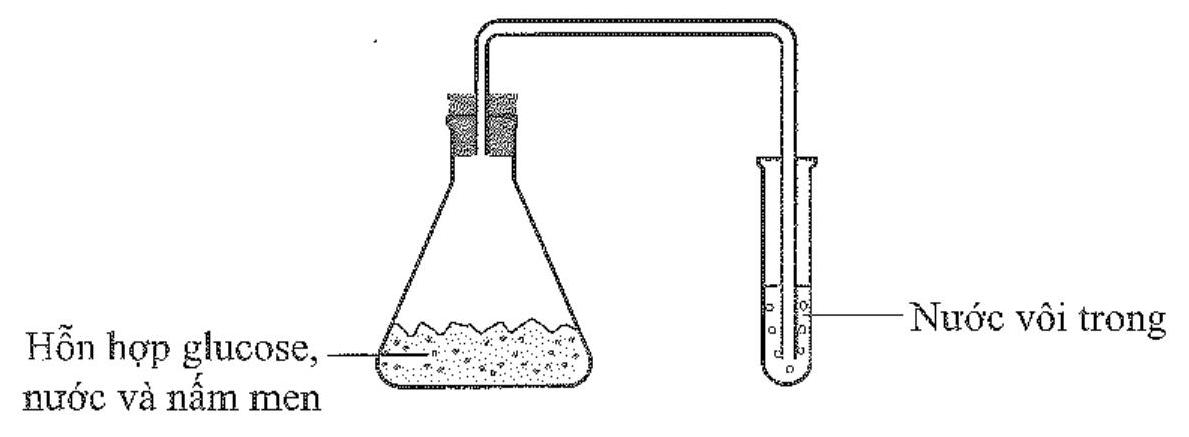
\includegraphics[width=\textwidth]{2025_10_23_80c1361fcdcd395cad8eg-13}
\captionsetup{labelformat=empty}
\caption{Hìmh 4.1. Mô phỏng thí nghiệm thử tính chất của sản phẩm từ lên men glucose}
\end{center}
\end{figure}

4.16. Viết phương trình hoá học của phản ứng giữa glucose với methanol khi có hydrogen chloride làm xúc tác. Giải thích vì sao phản ứng này không xảy ra với glucose ở dạng mạch hở.\\
4.17. Vinyl acetate được dùng để tổng hợp poly(vinyl acetate), một loại polymer được sử dụng nhiều trong công nghiệp gỗ, công nghiệp dệt,... Vinyl acetate có thể được tồng hợp hoàn toàn từ sinh khối (tinh bột hoặc cellulose). Viết các phương trình hoá học để tổng hợp vinyl acetate từ cellulose.\\
4.18. Chất X là thành phần chính của bông vải. Cho chất X tác dụng với hỗn hợp $\mathrm{HNO}_{3}$ và $\mathrm{H}_{2} \mathrm{SO}_{4}$ đặc để điều chế chất $\mathbb{Y}$ dùng làm vecni, phim ảnh,... Hàm lượng nitrogen trong chất Y khoảng $11,12 \%$. Xác định công thức phân tử chất Y và viết phương trình hoá học của phản ứng tạo thành chất Y từ chất X.\\
4.19. Theo Tiêu chuẩn Việt Nam TCVN 7624:2007, khi chế tạo gương, chiều dày lớp bạc phủ trên bề mặt tấm kính (quy ra tổng lượng bạc trên một đơn vị $\mathrm{m}^{2}$ kính) phải đạt tối thiểu $0,7 \mathrm{~g} \mathrm{~m}^{-2}$. Một công ty cần sản xuất $10000 \mathrm{~m}^{2}$ gương có độ dày lớp bạc phủ ở mức $0,72 \mathrm{~g} \mathrm{~m}^{-2}$. Biết rằng lớp bạc được tạo thành qua phản ứng giữa silver nitrate và glucose trong điều kiện thích hợp với hiệu suất phản ứng $90 \%$. Tính lượng silver nitrate và lượng glucose cần sử dụng để sản xuất $10000 \mathrm{~m}^{2}$ gương trên.\\
4.20*. Hàm lượng glucose có trong mẫu dược phẩm có thể được xác định bằng phương pháp chuẩn độ với iodine như sau: Cho một thể tích chính xác dung dịch chứa glucose vào một thể tích chính xác và dư nước iodine. Sau đó, thêm vào dung dịch sau phản ứng vài giọt dung dịch $\mathbb{X}$, rồi vừa lắc vừa nhỏ từ từ dung dịch sodium thiosulfate $\left(\mathrm{Na}_{2} \mathrm{~S}_{2} \mathrm{O}_{3}\right)$ có nồng độ xác định vào dung dịch ở trên đến khi mất màu xanh thì dừng lại. Ghi thể tích dung dịch sodium thiosulfate đã tiêu tốn. Biết rằng, glucose phản ứng với iodine tương tự như với bromine và phản ứng giữa iodine với sodium thiosulfate xảy ra như sau:

$$
\mathrm{I}_{2}+2 \mathrm{Na}_{2} \mathrm{~S}_{2} \mathrm{O}_{3} \rightarrow 2 \mathrm{NaI}+\mathrm{Na}_{2} \mathrm{~S}_{4} \mathrm{O}_{6}
$$

a) Viết phương trình hoá học của phản ứng giữa glucose và iodine.\\
b) Dự đoán chất X trong thí nghiệm trên là gì và X có vai trò gì trong thí nghiệm.\\
c) Trình bày nguyên tắc xác định hàm lượng glucose trong thí nghiệm trên.

\section*{CHỦ DỀ 3 HỢP CHÁT CHỨA NITROGEN}
\section*{Bal 5 AMINE}
5.1. Điền các từ hoặc cụm từ trong khung vào chỗ trống của các phát biểu sau cho phù hợp (mỗi từ hoặc cụm từ có thể điền vào một hoặc nhiều chỗ trống).\\
amine, base, hai, khi, hydrogen, acid, alcohol, alkyl halide, xanh, môt\\
a) Khi thay thế một hay nhiều nguyên tử ...(1)... trong phân tử ammonia bằng một hay nhiều gốc hydrocarbon, ta thu được hợp chất ...(2).... Tuỳ thuộc vào số nguyên tử ...(3)... bị thay thế mà có ...(4)... bậc khác nhau. Trên nguyên tử nitrogen còn ...(5)... cặp electron hoá trị riêng.\\
b) Các amine có tính chất chung là tính ...(6)... nên amine tác dụng được với ...(7)... tạo muối và một số dung dịch amine làm quỳ tím chuyển màu ...(8)....\\
c) Có thể điều chế alkylamine các bậc bằng cách cho ammonia tác dụng với ...(9)... theo tỉ lệ mol thích hợp.\\
5.2. Để rửa sạch chai lọ đựng aniline, nên dùng cách nào sau đây?\\
A. Rửa bằng xà phòng.\\
B. Rửa bằng nước.\\
C. Rửa bằng dung dịch NaOH , sau đó rưa lại bằng nước.\\
D. Rửa bằng dung dịch HCl , sau đó rửa lại bằng nước.\\
5.3. Mùi tanh của cá là hỗn hợp các amine và một số tạp chất khác. Để khử mùi tanh của cá trước khi chế biến thực phẩm, nên áp dụng cách nào sau đây?\\
A. Ngâm cá trong nước để amine tan vào nước.\\
B. Rửa cá bằng giấm ăn.\\
C. Rửa cá bằng dung dịch soda ( $\mathrm{Na}_{2} \mathrm{CO}_{3}$ ).\\
D. Rửa cá bằng dung dịch nước muối.\\
5.4. Cho các amine có công thức cấu tạo dưới đây:\\
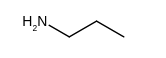
\includegraphics{smile-a5353e20d7f6a8ebab45a8caf662912e1411527a}\\
(1)\\
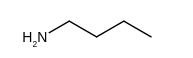
\includegraphics{smile-b6002fb21f271fdc098bc0632ec42e390641ec80}\\
(2)\\
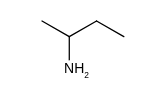
\includegraphics{smile-8f4e625d8f3ff0f9957a43fed99d795be59aae1a}\\
(3)\\
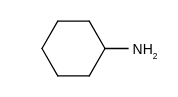
\includegraphics{smile-d77641550f289396fe80ada4bc918180ecd7d043}\\
(4)\\
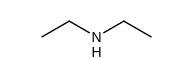
\includegraphics{smile-9e219d6ed6648fbc2d74729d0b21e6a2531e5720}\\
(5)\\
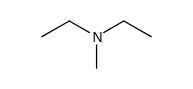
\includegraphics{smile-89bf3d1b0fdb353ce8bb474dbdcab9f183367b26}\\
(6)

Mỗi phát biểu sau đây là đúng hay sai?\\
(a) Trong số các amine trên, có 4 amine bậc một.\\
(b) Trong số các amine trên, có 2 amine bậc hai.\\
(c) Chất (4) là amine thom.\\
(d) Trong số các amine trên, có I amine bậc ba.\\
5.5. Kết quả phân tích nguyên tố của hợp chất amine thơm X có phần trăm khối lương các nguyên tố như sau: $\% \mathrm{C}=78,51 \% ; \% \mathrm{H}=8,41 \% ; \% \mathrm{~N}=13,08 \%$. Từ phổ khối lượng (MS) xác định được phân tử khối của X bằng 107. Ứng với công thức phân tử của X , có bao nhiêu amine thơm bậc một, kể cả X ?\\
A. 2 .\\
B. 1 .\\
C. 4 .\\
D. 3 .\\
5.6. Mỗi phát biểu sau đây là đúng hay sai?\\
(a) Trong phân tử amine, nguyên tử N liên kết với ít nhất một gốc hydrocarbon.\\
(b) Amine có tính base gây ra bởi cặp electron tự do trên nguyên tử N.\\
(c) Amine có tính khử do nguyên tử $N$ trong nhóm chức amine có số oxi hoá -3 .\\
(d) Trong phân tử amine bậc một có một nguyên tử N liên kết với chỉ một nguyên tữ H .\\
5.7. Phát biểu nào sau đây về methylamine và methane là đúng?\\
A. Trong cùng điều kiện về áp suất, nhiệt độ sôi của methylamine cao hơn của methane.\\
B. Giữa các phân tử methylamine không tạo được liên kết hydrogen.\\
C. Ở điều kiện thường, methylamine là chất lỏng và methane là chất khí.\\
D. Methylamine và methane đều tan kém trong nước.\\
5.8. Nicotine là chất gây nghiện có trong thuốc lá. Nicotine là một amine và có công thức cấu tạo như hình bên. Công thức phân tữ của nicotine là\\
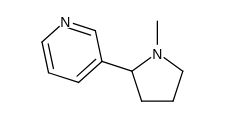
\includegraphics{smile-2dde04ad7f425d003d72e9ba212ddfcd82fa843e}\\
A. $\mathrm{C}_{10} \mathrm{H}_{12} \mathrm{~N}_{2}$.\\
B. $\mathrm{C}_{10} \mathrm{H}_{14} \mathrm{~N}_{2}$.\\
C. $\mathrm{C}_{12} \mathrm{H}_{14} \mathrm{~N}_{2}$.\\
D. $\mathrm{C}_{12} \mathrm{H}_{12} \mathrm{~N}_{2}$.\\
5.9. Nhỏ dung dịch của mỗi chất methylamine, ethylamine, ammonia, aniline vào các mầu giấy quỳ tím riêng rẽ. Số trường hợp mẩu giấy quỳ tỉm bị chuyển thành màu xanh là\\
A. 4 .\\
B. 3 .\\
C. 2 .\\
D. 1 .\\
5.10. Vỉ tanh của cá, đặc biệt là cá mè, là do các amine gây ra, trong đó có amine X . Phân tích nguyên tố đối với X thu được kết quả: $\% \mathrm{C}=61,02 \%$; $\% \mathrm{H}=15,25 \% ; \% \mathrm{~N}=23,73 \%$ (về khối lượng). Từ phổ khối lượng, xác định được phân tử khối của X bằng 59. Bằng các phương pháp khác, thấy phân tử X có cấu trúc đối xứng cao. Mỗi phát biểu sau đây là đúng hay sai?\\
(a) Công thức phân tử của X là $\mathrm{C}_{3} \mathrm{H}_{9} \mathrm{~N}$.\\
(b) Tên cúa $\mathbb{X}$ là propylamine.\\
(c) Công thức cấu tạo của X là $\left(\mathrm{CH}_{3}\right)_{3} \mathrm{~N}$.\\
(d) Khi cho dung dịch nitrous acid vào dung dịch $X$ thấy có khí nitrogen thoát ra.\\
5.11. Mỗi phát biểu sau đây là đúng hay sai?\\
(a) Nhỏ từ từ đến dư dung dịch methylamine $5 \%$ vào ống nghiệm chứa dung dịch $\mathrm{CuSO}_{4} 1 \%$, thấy trong ống nghiệm xuất hiện dung dịch màu xanh tím.\\
(b) Nhỏ nước bromine vào ống nghiệm chưa dung dịch nước của aniline thấy có kết tủa trắng xuất hiện.\\
(c) Cho từ từ dung dịch ethylamine vào ống nghiệm chưa dung dịch hỗn hợp acid HCl và $\mathrm{NaNO}_{2}$ ở nhiệt độ thấp $\left(0-5^{\circ} \mathrm{C}\right)$, thấy có khí không màu bay lên.\\
(d) Cho từ từ dung dịch ethylamine vào ống nghiệm chứa dung dịch hỗn hợp acid HCl và $\mathrm{NaNO}_{2}$ ở nhiệt độ thường, thu được ethanol.\\
5.12. Cho các amine là đồng phân cấu tạo của nhau có cùng công thức phân tử $\mathrm{C}_{4} \mathrm{H}_{11} \mathrm{~N}$.\\
a) Viết công thức cấu tạo của các amine.\\
b) Trong các amine trên, amine nào là amine bậc một, bậc hai, bậc ba?\\
c) Gọi tên theo danh pháp thay thế của các amine bậc một trong số các amine trên.\\
5.13. Aniline có thể được tổng hợp từ benzene theo sơ đồ chuyển hoá sau:\\
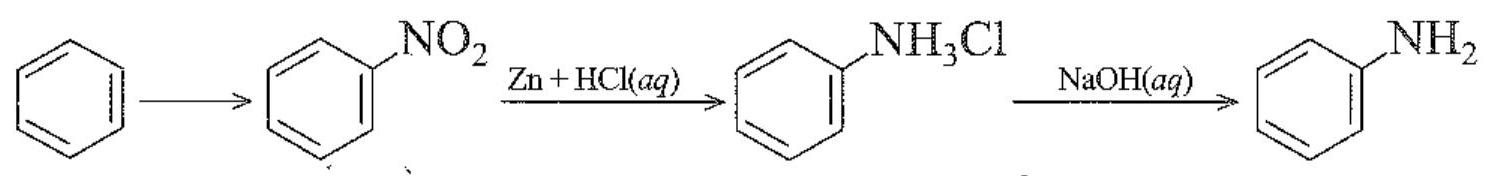
\includegraphics[max width=\textwidth, center]{2025_10_23_80c1361fcdcd395cad8eg-18}

Viết phương trình hoá học của các phản ứng theo sơ đồ trên.

\section*{311 \\
 6 AMINO ACID}
6.1. Cho các hợp chất cớcông thức cấu tạo dưới đây:\\
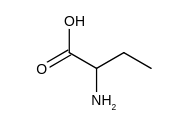
\includegraphics{smile-ce9e107623c4f6533182e192faf7704e6b49d5d0}\\
(1)\\
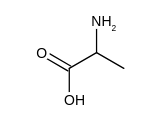
\includegraphics{smile-78e0b1cf0ee2c5260eadab7356b4644d14cf33b4}\\
(2)\\
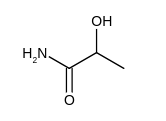
\includegraphics{smile-25199bebebe91f9def116b1be3d2b7f303d7c668}\\
(3)\\
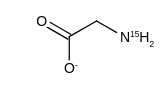
\includegraphics{smile-4c3a3eed75e33356ae6d0435650dfe31e8907c8e}\\
(4)

Những hợp chất nào trong số các chất trên thuộc loại $\alpha$-amino acid?\\
A. Chất (2), chất (3) và chất (4).\\
B. Chất (1) và chất (2).\\
C. Chất (1) và chất (3).\\
D. Chất (1), chất (2) và chất (4).\\
6.2. Chất nào dưới đây không phải là amino acid?\\
A. Lysine.\\
B. Glycine.\\
C. Aniline.\\
D. Glutamic acid.\\
6.3. Leucine có công thức cấu tạo $\mathrm{HOOCCH}\left(\mathrm{NH}_{2}\right) \mathrm{CH}_{2} \mathrm{CH}\left(\mathrm{CH}_{3}\right)_{2}$, là $\alpha$-amino acid có khả năng điều hoà sự tổng hợp protein của cơ. Tên theo danh pháp thay thế của leucine là\\
A. 2-aminoisohexanoic acid.\\
B. 2-amino-4-methylpentanoic acid.\\
C. 4-amino-2-methylpentanoic acid.\\
D. 2-amino-isohexanoic acid.\\
6.4. Các amino acid tồn tại ở trạng thái ion lưỡng cực, do đó chúng\\
A. có nhiệt độ nóng chảy cao và tan tốt trong nước.\\
B. có nhiệt độ nóng chảy cao và ít tan trong nước.\\
C. dễ nóng chảy và tan tốt trong nước.\\
D. dễ nóng chảy và ít tan trong nước.\\
6.5. Cho các chất có công thức cấu tạo sau: $\mathrm{H}_{2} \mathrm{NCH}_{2} \mathrm{COOH}$ (1); $\mathrm{C}_{2} \mathrm{H}_{5} \mathrm{COOH}$ (2); $\mathrm{C}_{2} \mathrm{H}_{5} \mathrm{NH}_{2}$ (3) $; \mathrm{H}_{2} \mathrm{NCH}_{2} \mathrm{CH}_{2} \mathrm{CH}\left(\mathrm{NH}_{2}\right) \mathrm{COOH}$ (4); $\mathrm{C}_{6} \mathrm{H}_{5} \mathrm{NH}_{2}$ (5).\\
Những chất vừa phản ứng được với acid vừa phản ứng được với base là\\
A. (1), (2).\\
B. (4), (5).\\
C. (2), (3).\\
D. (1), (4).\\
6.6. Cho dung dịch chứa amino acid $\mathbb{X}$ tồn tại ở dạng ion lưỡng cực:\\
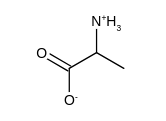
\includegraphics{smile-e0d9861e09b1f028307d4be060a3fe07dfc1351b}

Đặt dung dịch này trong một điện trường. Khi đó:\\
A. Chất X sẽ di chuyển về phía cực âm của điện trường.\\
B. Chất $X$ sẽ di chuyển về phía cực dương của điện trường.\\
C. Chất X không di chuyển dưới tác dụng của điện trường.\\
D. Chất X chuyển hoàn toàn về dạng $\mathrm{H}_{2} \mathrm{NCH}(\mathrm{R}) \mathrm{COOH}$.\\
6.7. Kết quả phân tích nguyên tố của một amino acid X như sau: $\% \mathrm{C}=46,60 \%$; $\% \mathrm{H}=8,74 \% ; \% \mathrm{~N}=13,59 \%$ (về khối lượng); còn lại là oxygen. Bằng phổ khối lượng (MS), xác định được phân tử khối của X bằng 103. Phát biểu nào sau đây là không đúng?\\
A. Công thức phân tử của X là $\mathrm{C}_{4} \mathrm{H}_{9} \mathrm{O}_{2} \mathrm{~N}$.\\
B. Có $2 \alpha$-amino acid đồng phân cấu tạo ứng với công thức phân tử của X .\\
C. Có 3 chất đồng phân cấu tạo có cùng công thức phân tử với $\mathbf{X}$ tạo được dung dịch có môi trường base.\\
D. Khi đặt X được điều chỉnh đến $\mathrm{pH}=6,0$ trong điện trường thì X sẽ di chuyển về cực âm.\\
6.8. Thuỷ phân tripeptide X bằng xúc tác enzyme thu được hỗn hợp gồm alanine, lysine và glutamic acid. Đặt hỗn hợp sản phẩm trong điện trường ở $\mathrm{pH}=6,0$. Phát biểu nào sau đây về sự di chuyển của các amino acid dưới tác dụng của điện trường là đúng?\\
A. Cả ba amino acid đều di chuyển về phía cực âm.\\
B. Cả ba amino acid đều di chuyển về phía cực dương.\\
C. Có hai amino acid di chuyển về phía cực âm.\\
D. Một amino acid không di chuyển; mỗi một điện cực có một amino acid di chuyển về.\\
6.9. Mỗi phát biểu sau đây là đúng hay sai?\\
(a) Khi thay nguyên tử H trong phân tử hydrocarbon bằng nhóm amino và nhóm carboxyl, thu được hợp chất amino acid.\\
(b) Trong phân tữ amino acid có đồng thời nhóm amino và nhóm carboxyl.\\
(c) Úng với công thức phân tử $\mathrm{C}_{4} \mathrm{H}_{9} \mathrm{NO}_{2}$ có $2 \alpha$-amino acid là đồng phân cấu tạo của nhau.\\
(d) Alanine và glycine là các amino acid thiên nhiên.\\
6.10. Mỗi phát biểu sau là đúng hay sai?\\
(a) Trong dung dich, các amino acid tồn tai theo cân bằng:\\
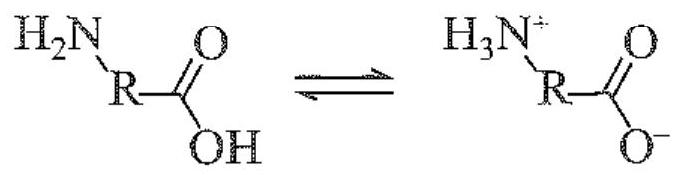
\includegraphics[max width=\textwidth, center]{2025_10_23_80c1361fcdcd395cad8eg-20}\\
(b) Đa số các amino acid tinh khiết tồn tại ở trạng thái rắn.\\
(c) Các amino acid thường tan kém trong nước.\\
(d) Các amino acid có nhiệt độ nóng chảy cao hơn các chất hữu cơ có khối lượng mol phân tử tương đương.\\
6.11. Mỗi phát biếu sau đây là đúng hay sai?\\
(a) Tất cả các amino acid đều có thể tham gia phản ứng trùng ngưng tạo ra polypeptide.\\
(b) Dung dịch của glycine không làm đồi màu quỳ tím.\\
(c) Ở trạng thái tinh khiết, các amino acid tồn tại ở dạng muối $\mathrm{H}_{3} \mathrm{~N}^{+} \mathrm{RCOO}^{-}$.\\
(d) Khi đặt dung dịch glycine trong một điện trường, glycine chuyển dịch về phía cực âm.\\
6.12. Từ amino acid $X$ và methyl alcohol điều chế được ester $Y$ có công thức phân tử $\mathrm{C}_{3} \mathrm{H}_{7} \mathrm{O}_{2} \mathrm{~N}$. Công thức cấu tạo của amino acid X là\\
A. $\mathrm{CH}_{3} \mathrm{CH}_{2} \mathrm{COOH}$.\\
B. $\mathrm{H}_{2} \mathrm{NCH}_{2} \mathrm{COOH}$.\\
C. $\mathrm{H}_{2} \mathrm{NCH}_{2} \mathrm{COOCH}_{3}$.\\
D. $\mathrm{CH}_{3} \mathrm{CH}\left(\mathrm{NH}_{2}\right) \mathrm{COOH}$.\\
6.13. Cho các chất có công thúc cấu tạo sau: $\mathrm{HOOCCH}_{2} \mathrm{CH}\left(\mathrm{NH}_{2}\right) \mathrm{COOH}_{\text {, }} \mathrm{H}_{2} \mathrm{NCH}_{2} \mathrm{COOH}, \mathrm{H}_{2} \mathrm{NCH}_{2} \mathrm{CH}\left(\mathrm{NH}_{2}\right) \mathrm{COOH}, \mathrm{H}_{2} \mathrm{NCH}_{2} \mathrm{CH}_{2} \mathrm{COOH}$. Dự doán môi trường (acid, base, trung tính) của dung dịch mỗi amino acid trên. Giải thích.\\
6.14. Cho các dung dịch sau: hồ tinh bột, methylamine, glucose và glycine được kí hiệu ngẫu nhiên là $\mathrm{X} 1, \mathrm{X} 2, \mathrm{X} 3$ và X 4 . Một học sinh tiến hành các thí nghiệm để phân biệt từng chất trong số các chất trên và có kết quả thí nghiệm sau:

\begin{center}
\begin{tabular}{|l|l|l|}
\hline
Dung dich & Thuóc thu & Hiên tương \\
\hline
X1 & Phenolphthalein & Chuyển màu hồng \\
\hline
X2 & Dung dịch $\mathrm{I}_{2} / \mathrm{KI}$ & Xuất hiện màu xanh tím \\
\hline
X3 & $\mathrm{Cu}(\mathrm{OH})_{2}$ & Tạo dung dịch màu xanh lam \\
\hline
X4 & Phenolphthalein & Dung dịch không đổi màu \\
\hline
\end{tabular}
\end{center}

Tự kết quả trên, hãy cho biết $\mathrm{X} 1, \mathrm{X} 2, \mathrm{X} 3$ và X 4 tương úng là những chất nào trong số các chất trên.

\section*{Bat \\
 7. PEPTIDE, PROTEIN VÀ ENZYME}
7.1. Cho các chất có công thức cấu tạo sau:\\
(1)\\
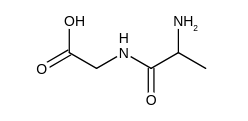
\includegraphics{smile-d5ede381df55cc8a6df7babb2182e99baa2a6392}\\
(2)\\
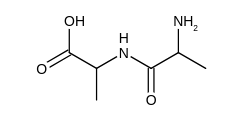
\includegraphics{smile-2149c9af4dce087056af9eaa6d7e3cab32ae50c6}\\
(3)\\
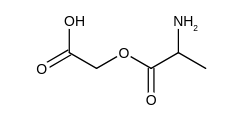
\includegraphics{smile-9c9cb2317cf9ecc7e76f30cf5e40116eea34611b}\\
(4)\\
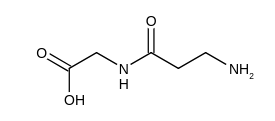
\includegraphics{smile-ee574251b1cea5ca6d39d8f48566b3453006fd18}

Trong các hợp chất trên, những hợp chất nào thuộc loại dipeptide?\\
A. Hợp chất (1) và (2).\\
B. Hợp chất (1) và (3).\\
C. Hợp chất (2) và (3).\\
D. Hợp chất (2) và (4).\\
7.2. Trong cấu trúc phân tử của chất cho ở hình bên, liên kết peptide là\\
A. liên kết (1).\\
B. liên kết (3).\\
C. liên kết (2).\\
D. liên kết (4).\\
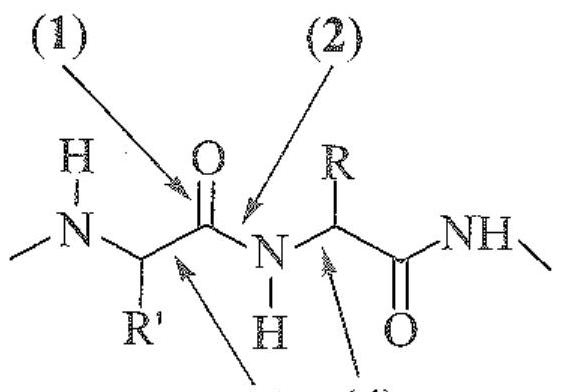
\includegraphics[max width=\textwidth, center]{2025_10_23_80c1361fcdcd395cad8eg-21}\\
(3) (4)\\
7.3. Một tripeptide X được cấu thành từ 2 phân tử Ala và 1 phân tử Gly. Công thức cấu tạo của $\mathbf{X}$ không thể là\\
A. Ala-Ala-Gly.\\
B. Ala-Gly-Ala.\\
C. Gly-Ala-Ala.\\
D. Gly-Ala-Gly.\\
7.4. Cho peptide X có công thức cấu tạo sau:\\
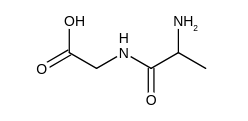
\includegraphics{smile-ba6876f29ed81fab0d2d80990e0937af4318ddd1}

Khi thuỷ phân hoàn toàn X trong môi trường NaOH thu được sản phẩm hữu cơ có công thức là\\
A. $\mathrm{H}_{2} \mathrm{NCH}\left(\mathrm{CH}_{3}\right) \mathrm{COOH}$ và $\mathrm{H}_{2} \mathrm{NCH}_{2} \mathrm{COOH}$.\\
B. $\mathrm{H}_{2} \mathrm{NCH}\left(\mathrm{CH}_{3}\right) \mathrm{COONa}$ và $\mathrm{H}_{2} \mathrm{NCH}_{2} \mathrm{COONa}$.\\
C. $\mathrm{H}_{2} \mathrm{NCH}\left(\mathrm{CH}_{3}\right) \mathrm{COONa}$ và $\mathrm{H}_{2} \mathrm{NCH}_{2} \mathrm{COOH}$.\\
D. $\mathrm{H}_{2} \mathrm{NCH}\left(\mathrm{CH}_{3}\right) \mathrm{COOH}$ và $\mathrm{H}_{2} \mathrm{NCH}_{2} \mathrm{COONa}$.\\
7.5. Cho các peptide sau: Gly-Val-Ala-Gly (1); Ala-Gly (2); Val-Gly-Ala (3); Gly-Val-Ala (4). Những peptide nào có phản ứng tạo màu biuret với $\mathrm{Cu}(\mathrm{OH})_{2}$ trong môi trường kiềm?\\
A. (1), (2).\\
B. (2), (3) và (4).\\
C. (1), (3) và (4).\\
D. (3) và (4).\\
7.6. Phát biểu nào sau đây là không đúng?\\
A. Khi bị đun nóng, lòng trắng trứng chuyển từ trạng thái lỏng sang trạng thái rắn.\\
B. Protein là chuỗi polypeptide được tạo thành từ nhiều đơn vị $\alpha$-amino acid.\\
C. Albumin trong lòng trắng trứng là protein có dạng hình sợi và không tan trong nước.\\
D. Khi nhỏ nitric acid vào lòng trắng trứng, màu trắng của lòng trắng trứng chuyển thành màu vàng.\\
7.7. Các enzyme đóng vai trò quan trọng đối với cơ thể sinh vật, như xúc tác cho các quá trình sinh hoá và hoá học. Ví dụ, lipase là enzyme xúc tác cho quá trình thuỷ phân các chất béo chuỗi dài; protease là enzyme xúc tác cho quá trình thuỷ phân các liên kết peptide có trong protein và polypeptide;...

Các enzyme chỉ tồn tại và phát triển ở môi trường gần trung tính và nhiệt độ tương đối thấp (gần với nhiệt độ của cơ thể sinh vật). Khi đóng vai trò là chất xúc tác trong các quá trình sinh hoá, các enzyme không có đặc điểm nào sau đây?\\
A. Có tính chọn lọc cao.\\
B. Làm tăng tốc độ của các quá trình sinh hoá.\\
C. Có tác dụng tốt ở nhiệt độ cao hoặc môi trường acid mạnh.\\
D. Chỉ hoạt động trong điều kiện nhiệt độ phù hợp.\\
7.8. Mỗi phát biểu sau là đúng hay sai?\\
(a) Tất cả các peptide đều có thể tạo phức chất màu tím với $\mathrm{Cu}(\mathrm{OH})_{2} / \mathrm{NaOH}$.\\
(b) Dung dịch của dipeptide Ala-Gly không làm đổi màu quỳ tím.\\
(c) Từ $3 \alpha$-amino acid khác nhau có thể tạo được 3 tripeptide.\\
(d) Khi thuỷ phân hoàn toàn polypeptide thu được hỗn hợp các $\alpha$-amino acid.\\
7.9. Mỗi phát biểu về các protein sau đây là đúng hay sai?\\
(a) Tất cả các loại protein đều không tan trong nước.\\
(b) Có thể sử dụng phản ứng màu biuret để nhận biết sự có mặt của protein.\\
(c) Protein có thể tạo hợp chất màu vàng khi tác dụng với nitric acid.\\
(d) Khi thuỷ phân hoàn toàn protein thu được hỗn hợp các $\alpha$-amino acid.\\
7.10. Khi phân tích nguyên tố của một dipeptide X thu được phần trăm khối lượng của các nguyên tố như sau: $\% \mathrm{C}=41,10 \% ; \% \mathrm{H}=6,85 \% ; \% \mathrm{~N}=19,18 \%$; còn lại là oxygen. Từ phổ khối lượng (MS) xác định được phân tử khối của X bằng 146. Công thức cấu tạo của X có thể là\\
A. $\mathrm{H}_{2} \mathrm{NCH}_{2} \mathrm{CONHCH}\left(\mathrm{CH}_{3}\right) \mathrm{COOH}$.\\
B. $\mathrm{H}_{2} \mathrm{NCH}_{2} \mathrm{CH}_{2} \mathrm{CONHCH}\left(\mathrm{CH}_{3}\right) \mathrm{COOH}$.\\
C. $\mathrm{H}_{2} \mathrm{NCH}_{2} \mathrm{CONHCH}_{2} \mathrm{CH}_{2} \mathrm{COOH}$.\\
D. $\mathrm{H}_{2} \mathrm{NCH}_{2} \mathrm{CH}_{2} \mathrm{CONHCH}_{2} \mathrm{COOH}$.

\section*{CHỦ DỀ 4 POLYMER}
\section*{BAII 8. DAI CUONG VỀ POLYMER}
8.1. Điền các từ hoặc cưn từ trong khung vào chỗ trống của các phát biểu sau cho phụ̀ hợp (mỗi chỗ trống chỉ điền một từ hoặc cụm từ).\\
rán, $\mathrm{CH}_{2}=\mathrm{CH}_{2}$ không tan, mát xich, tring hop, cong hop, $\mathrm{CH}_{2}$, long, phân tú khôl, trùng ngung, không, hê số polymer hoá, có tan, polymer\\
a) Polymer là những hợp chất hữu cơ có ...(1)... lớn, do nhiều ...(2)... liên kết với nhau tạo nên.\\
b) Trong công thức của chất dẻo PE thì $-\left(\mathrm{CH}_{2}-\mathrm{CH}_{2}\right)_{\mathrm{n}}$ được gọi là ...(3)..., giá trị n được gọi là ... (4)... và monomer là ... (5)....\\
c) Ở điều kiện thường, hầu hết các polymer là chất ...(6)... và ...(7)... bay hoi, ...(8)... trong dung môi thông thường.\\
d) Chất déo polyethylene được điều chế bằng phản ứng ...(9)... và tơ nylon-6,6 được điều chế bằng phản ứng ...(10)....\\
8.2. Hãy ghép thông tin công thức của polymer ở cột A với tên gọi thích hợp ở cột B .

\section*{Côt A}
1.

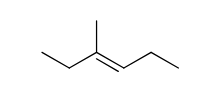
\includegraphics{smile-39d46c01f47b85c0d4dbb475b16ebf35911e8222}\\
2.

$$
-\left(\mathrm{NH}\left[\mathrm{CH}_{2}\right]_{5} \mathrm{CO}\right)_{\mathrm{n}}
$$

3.

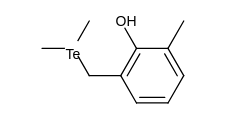
\includegraphics{smile-6de4c5775daa69ec968e49b913836da06a23e61e}\\
4. $\quad\left(\mathrm{NH}\left[\mathrm{CH}_{2}\right]_{6} \mathrm{NHCO}\left[\mathrm{CH}_{2}\right]_{4} \mathrm{CO}\right)_{n}$\\
5.\\
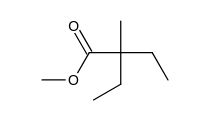
\includegraphics{smile-bba4c2c0db5658f9cca3f2d10ca7bb9942bf1d8d}\\
b) Poly(methyl methacrylate)\\
c) Nylon-6,6\\
d) Capron

\section*{Côt $\frac{B}{B}$}
a) Poly(phenol-formaldehyde)\\
b) Poly(methyl methacrylate)\\
c) Nylon-6,6\\
capron\\
e) Polyisoprene\\
8.3. Hãy ghép đặc điểm ở cột A với ví dụ polymer ở cột B cho phù hợp.

\section*{Côt A}
\begin{enumerate}
  \item Polymer có tham gia phản ứng cộng hợp
  \item Polymer thành phần có chứa nguyên tố oxygen
  \item Polymer được điều chế bằng phản ứng trùng hợp
  \item Polymer được điều chế bằng phản ứng trùng ngưng
\end{enumerate}

\section*{Cột B}
a) Poly(methyl methacrylate)\\
b) Polypropylene\\
c) Nylon-6,6\\
d) Polyisoprene.\\
5. Polymer thuộc loại polymer nhiệt dẻo\\
e) Poly(vinyl chloride)\\
8.4. Loại polymer nào sau đây có chưa nguyên tố nitrogen?\\
A. Polystyrene.\\
B. Poly(vinyl chloride).\\
C. Polyisoprene.\\
D. Nylon-6,6.\\
8.5. Polymer nào sau đây trong thành phần chỉ gồm hai nguyên tố C và H ?\\
A. Poly(phenol-formaldehyde).\\
B. Poly(methyl methacrylate).\\
C. Polybuta-1,3-diene.\\
D. Nylon-6,6.\\
8.6. Quá trình cộng hợp liên tiếp nhiều phân tử nhỏ giống nhau hoặc tương tự nhau (monomer) tạo thành phân tử lớn (polymer) được gọi là phản ứng\\
A. thuỷ phân.\\
B. trùng hợ.\\
C. trùng ngưng.\\
D. xà phòng hoá.\\
8.7. Quá trình kết hợp nhiều phân tử nhỏ (monomer) thành phân tử lớn (polymer), đồng thời giải phóng nhữug phân tử nhỏ khác (thường là $\mathrm{H}_{2} \mathrm{O}$ ) được gọi là phản úng\\
A. trùng hợp.\\
B. thế.\\
C. tách.\\
D. trùng ngưng.\\
8.8. Khi phân tích thành phần một polymer X thấy tỉ lệ số mol C và H tương ứng là $1: 1$. X là polymer nào dưới đây?\\
A. Polypropylene.\\
B. Tinh bột.\\
C. Polystyrene.\\
D. Poly(vinyl chloride).\\
8.9. Phân tử khối của một đoạn mạch cellulose là 2430000 . Số lượng mắt xích trong doạn mạch cellulose nêu trên là\\
A. 15000 .\\
B. 12500 .\\
C. 12000 .\\
D. 16000 .\\
8.10. Phản ứng $\left.\mathrm{nCH}_{2}=\mathrm{CH}-\mathrm{CH}=\mathrm{CH}_{2} \xrightarrow{\mathrm{xt}, \mathrm{t}^{\mathrm{a}}, \mathrm{p}}+\mathrm{CH}_{2}-\mathrm{CH}=\mathrm{CH}-\mathrm{CH}_{2}\right)_{\mathrm{n}}$ dùng để điều chế polymer nào sau đây?\\
A. Polypropylene.\\
B. Polyethylene.\\
C. Polybuta-1,3-diene.\\
D. Polystyrene.\\
8.11. Những phát biểu nào sau đây là đúng?\\
(a) Dựa vào nguồn gốc, polymer được chia thành: polymer thiên nhiên, polymer tổng hợp và polymer bán tổng hợp.\\
(b) Các polymer đều khá bền với dung dịch acid hoặc base.\\
(c) Những polymer khi đun nóng không bị nóng chảy mà bị phân huỷ thì được gọi là chất nhiệt rắn.\\
(d) Tất cả các polymer đều tham gia phản ứng phân cắt mạch polymer.\\
8.12. Poly(phenol-formaldehyde) (PPF) là polymer có tính cúng, chịu nhiệt, chống mài mòn và chống ẩm cao. Vì vậy, PPF được ứng dụng rộng rãi trong nhiều ngành công nghiệp như sử dụng làm chất kết dính trong sản xuất ván ép, ván MDF , giúp tăng độ bền và khả năng chống ẩm của vật liệu. PPF được điều chế từ phản ứng giữa phenol và formaldehyde ở pH và nhiệt độ thích hợp. Mỗi phát biểu sau đây là đúng hay sai?\\
(a) PPF được điều chế từ phản ứng trùng hợp.\\
(b) Các mạch polymer của PPF có thể tham gia phản ứng nối mạch polymer lại với nhau tạo thành mạng không gian.\\
(c) Rác thải nhựa làm từ vật liệu PPF có thể xử lí bằng cách đốt.\\
(d) PPF là vật liệu polymer thuộc loại chất dẻo.\\
8.13. Thuộc da là quá trình mà da động vật được chuyển hoá thành da thuộc với những đặc tính ưu việt hơn như chịu nhiệt độ cao, không thối rữa khi tiếp xúc với nước và các môi trường khác. Quá trình thuộc da xử lí với HCHO là phản ứng tăng mạch carbon của protein dưới tác dụng của HCHO tạo sản phẩm có cấu trúc không gian. Mỗi phát biểu sau là đúng hay sai?\\
(a) Polymer khâu mạch khó nóng chảy và khó hoà tan hơn polymer chưa khâu mạch.\\
(b) Ở phản ứng khâu mạch carbon, các mạch polymer nối lại với nhau tạo mạng không gian nên bền hơn.\\
(c) Phản ứng xảy ra ở trên thuộc loại phản ứng trùng ngưng.\\
(d) Khi đun nóng da động vật trong dung dịch NaOH , sẽ xảy ra phản ứng depolymer hoá.\\
8.14. Vật liệu polymer đã và đang được sử dụng rộng rãi trong rất nhiều lĩnh vực. Với những ưu điểm vượt trội về tính chất, độ bền,..., vật liệu polymer được ứng dụng rộng rãi trong đòi sống làm vật liệu cách điện và đặc biệt là vật liệu xây dựng mới như: sơn chống thấm, bê tông siêu nhẹ, gỗ công nghiệp,... Các polymer được điều chế bằng phản ứng trùng hợp hoặc trùng ngưng. Những phát biểu nào sau đây là đúng?\\
(a) Sự khác biệt cơ bản giữa hai loại phản ứng điều chế polymer là: phản ứng trùng ngưng có tạo ra các phân tử nhỏ, còn trùng hợp thì không tạo ra phân tử nhỏ.\\
(b) Trùng hợp buta-1,3-diene thu được polymer có cấu trúc tương tự cao su tự nhiên.\\
(c) Poly(vinyl acetate) (PVA) được dùng chế tạo son, keo dán. Monomer dùng để trùng hợp tạo PVA là $\mathrm{CH}_{2}=\mathrm{CHCOOCH}_{3}$.\\
(d) Nylon-6,6 được sử dụng phổ biến trong ngành dệt may và được điều chế từ phản ứng trùng ngưng.\\
8.15. Cellulose triacetate $\left(\mathrm{CTA},\left[\mathrm{C}_{6} \mathrm{H}_{7} \mathrm{O}_{2}\left(\mathrm{OOCCH}_{3}\right)_{3}\right]_{\mathrm{n}}\right)$ là polymer được sản xuất thương mại lần đầu tiên ở Mỹ vào năm 1954. Polymer này được sử dụng để sản xuất tơ sợi chống nhăn, màng cho màn hình tinh thể lỏng,... Một đoạn mạch cellulose triacetate có phân tử khối là 345600 thì chứa bao nhiêu mắt xích?\\
8.16. Polymer X được dùng làm vật liệu tơ polyamide có hệ số polymer hoá là 500 và có phân tử khối là 56500 . Biết mỗi mắt xích của $X$ chỉ có 1 nguyên tữ $N$. Hãy viết công thức cấu tạo của của polymer $X$.

\section*{Bat \\
 9. VÂT LIỆU POLYMER}
9.1. Polymer nào sau đây được dùng để chế tạo chất dẻo?\\
A. Polybuta-1,3-diene.\\
B. Poly(phenol-formaldehyde).\\
C. Polyisoprene.\\
D. Poly(urea-formaldehyde).\\
9.2. Polymer X là chất rắn trong suốt, có khả năng cho ánh sáng truyền qua tốt nên được dùng để chế tạo thuỷ tinh hữu co. Tên gọi của X là\\
A. poly(methyl methacrylate).\\
B. poly(phenol-formaldehyde).\\
C. polyethylene.\\
D. poly(vinyl chloride).\\
9.3. Polypropylene ( PP ) là chất dẻo thường được sử dụng để sản xuất các sản phẩm thiết bị y tế, đồ gia dụng,... Vật liệu được chế tạo từ PP thường có kí hiệu như hình bên, PP được tổng hợp từ monomer nào sau đây?\\
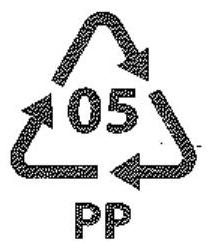
\includegraphics[max width=\textwidth, center]{2025_10_23_80c1361fcdcd395cad8eg-28}\\
A. $\mathrm{CH}_{2}=\mathrm{CH}_{2}$.\\
B. $\mathrm{CH}_{2}=\mathrm{CHCN}$.\\
C. $\mathrm{CH}_{3} \mathrm{CH}=\mathrm{CH}_{2}$.\\
D. $\mathrm{C}_{6} \mathrm{H}_{5} \mathrm{OH}$ và HCHO .\\
9.4. PVC là chất rắn vô định hình, cách điện tốt, bền với acid, được dùng làm vật liệu cách điện, ống dẫn nước, vải che mưa,... PVC được tổng hợp trực tiếp từ monomer nào sau đây?\\
A. Acrylonitrile.\\
B. Vinyl chloride.\\
C. Vinyl acetate.\\
D. Propylene.\\
9.5. Polystyrene (PS) là chất nhiệt dẻo thường được sử dụng để sản xuất đồ nhựa như li, chén dùng một lần hoặc hộp đựng thức ăn mang về tại các cưa hàng. Ở khoảng trên $80^{\circ} \mathrm{C}, \mathrm{PS}$ bị biến đồi trở nên mềm, dính. Do vậy, nên tránh hâm nóng thực phẩm chứa trong các loại hộp này. Monomer được dùng để điều chế PS là\\
A. $\bigcirc-\mathrm{CH}=\mathrm{CH}_{2}$.\\
B. $\mathrm{CH}_{2}=\mathrm{CHCH}=\mathrm{CH}_{2}$.\\
C. $\mathrm{CH}_{2}=\mathrm{CH}_{2}$.\\
D. $\mathrm{CH}_{2}=\mathrm{CHCH}_{3}$.\\
9.6. Với nhu cầu chế tạo vật liệu an toàn với môi trường, năm 2005 sản phẩm "hộp bã mía" - bao bì từ thực vật và an toàn cho sức khoẻ với nhiều tính năng vượt trội so với hộp xốp đã ra đời. Đây là loại bao bì có thành phần hoàn toàn tự nhiên, phần lớn là sợi bã mía từ nhà máy đường, với khả năng chịu nhiệt rộng từ -40 đến $200^{\circ} \mathrm{C}$, bền nhiệt trong lò ví sóng, lò nướng nên an toàn với sức khoẻ con người. Những phát biểu nào sau đây là đúng?\\
(a) Thành phần chính của hộp bã mía là cellulose.\\
(b) Hộp bã mía phân huỷ sinh học được nên thân thiện với môi trường.\\
(c) Hộp xốp đựng thức ăn nhanh làm từ chất dẻo PS cũng là vật liệu dễ phân huỷ sinh học.\\
(d) Hộp bã mía có thành phần chính là polymer thiên nhiên, hộp xốp từ chất dẻo là polymer tổng hợp.\\
9.7. Với sự phát triển của công nghệ hiện đại, vật liệu composite đã nhanh chóng được đưa vào sử dụng ở nhiều lĩnh vực khác nhau, nhất là ngành vật liệu mới. Đặc biệt là các vật liệu composite polymer với các đặc tính ưu việt như nhẹ, bền với môi trường ăn mòn, độ dẫn nhiệt và dẫn điện thấp. Do vậy, loại vật liệu này được sử dụng rộng rãi trong hàng không, xây dựng,... Ví dụ, $50 \%$ vật liệu chế tạo máy bay Boeing 787 là vật liệu composite. Những phát biếu nào sau đây là đúng?\\
(a) Sợi carbon được dùng làm vật liệu cốt trong composite do độ bền cao, nhẹ, kháng hoá chất, chịu được nhiệt độ cao và giãn nở nhiệt thấp.\\
(b) Vật liệu nền là chất dẻo giúp các pha gián đoạn liên kết được với nhau để tạo một khối kết dính và thống nhất, giúp bảo vệ vật liệu cốt, ồn định màu sắc, giữ được độ dẻo dai,...\\
(c) Thành phần của các vật liệu composite gồm một vật liệu nền và một vật liệu cốt.\\
(d) Vật liệu composite với cốt là bột gỗ được sử dụng làm ván lát sàn, cánh cưa, tấm ốp trong nội thất.\\
9.8. Hãy ghép thông tin ở cột A với vật liệu polymer thích hợp ở cột B .

\section*{Cột A}
\section*{1. Polymer có thành phần không chứa nguyên tữ nitrogen}
2. Polymer mà mỗi mắt xích đều tạo bởi bốn nguyên tố\begin{enumerate}
  \setcounter{enumi}{2}
  \item Polymer thành phần chính chưa protein
  \item Vật liệu polymer có nguồn gốc từ cellulose
  \item Vật liệu polymer thiên nhiên
  \item Polymer thuộc loại bán tổng hợp
\end{enumerate}

\section*{Côt B}
a) Sợi từ cây bông\\
b) To visco\\
c) To cellulose acetate\\
d) To capron\\
e) To olon\\
g) Tơ tằm\\
9.9. Sợi visco thuộc loại\\
A. polymer trùng ngưng.\\
B. polymer bán tổng hợp.\\
C. polymer thiên nhiên.\\
D. polymer tổng hợp.\\
9.10. Tơ sợi là một nguyên liệu quan trọng trong ngành dệt may và sản xuất vật liệu. Tơ sợi được sản xuất từ các nguồn nguyên liệu tự nhiên hoặc tổng hợp. Các loại tơ sợi phổ biến bao gồm tơ sợi tự nhiên như tơ tằm, lông cừu, sợi cotton và tơ sợi tổng hợp như nylon,...\\
Những phát biểu nào sau đây là đúng?\\
(a) Tơ nylon-6,6 và tơ capron thuộc loại tơ polyamide.\\
(b) Tơ nylon, tơ tằm, tơ visco đều bền với nhiệt độ.\\
(c) Quần áo được dệt bằng sợi len lông cừu, tơ tằm không nên giặt với xà phòng có độ kiềm cao.\\
(d) Tơ capron và tơ olon đều có thành phần chứa nhóm $-\mathrm{CO}-\mathrm{NH}-$.\\
9.11. Tơ visco được sản xuất phổ biến từ đầu thế kỉ XX , là một loại chất liệu được làm từ bột gỗ của cây như tre, đậu nành, mía,..., qua quá trình xử lí hoá học được sợi visco. Sợi visco thấm hút mồ hôi và thoáng khí, mềm mại nên rất phổ biến trong việc sản xuất quần áo, đặc biệt là trang phục mùa hè vì nó giúp người mặc cảm thấy mát mẻ và thoải mái. Những phát biểu nào sau đây là đúng?\\
(a) Tơ visco thuộc loại tơ thiên nhiên.\\
(b) Tơ visco thuộc loại tơ bán tổng hợp.\\
(c) Sợi visco có thành phần chính là cellulose đã được xử lí hoá chất.\\
(d) Tơ là vật liệu polymer hình sợi, dài, mảnh, có độ bền nhất định, mạch không nhánh.\\
9.12. Cao su isoprene được tổng hợp từ monomer nào sau đây?\\
A. $\mathrm{CH}_{2}=\mathrm{C}\left(\mathrm{CH}_{3}\right) \mathrm{CH}=\mathrm{CH}_{2}$.\\
B. $\mathrm{CH}_{3} \mathrm{CH}=\mathrm{C}=\mathrm{CH}_{2}$.\\
C. $\left(\mathrm{CH}_{3}\right)_{2} \mathrm{C}=\mathrm{C}=\mathrm{CH}_{2}$.\\
D. $\mathrm{CH}_{2}=\mathrm{CHCH}=\mathrm{CH}_{2}$.\\
9.13. Cao su buna-N được tổng hợp bằng cách trùng hợp buta-1,3-diene với chất nào sau đây?\\
A. Isoprene.\\
B. Natri.\\
C. Acrylonitrile.\\
D. Styrene.\\
9.14. Keo dán là vật liệu polymer\\
A. có khả năng kết dính hai mảnh vật liệu rắn với nhau.\\
B. có khả năng tạo liên kết hydrogen giữa các vật liệu được kết dính.\\
C. có thành phần gồm vật liệu cốt và vật liệu nền là chất kết dính.\\
D. có khả năng kết dính khi thểm chất đóng rắn.\\
9.15. Năm 1839, Charles Goodyear đã được cấp bằng sáng chế cho phát minh về quy trình hoá học để chế tạo ra cao su lưu hoá - một loại cao su có cấu trúc đặc biệt, bền cơ học, chịu được sự ma sát, va chạm, đàn hồi tốt và có thể đúc được. Những phát biểu nào sau đây là đúng?\\
(a) Cao su lưu hoá còn có tên gọi là cao su buna-S.\\
(b) Bản chất của việc lưu hoá cao su là tạo ra cầu nối disulfide -S-S- giữa các mạch cao su nên cao su lưu hoá có tính chất cơ lí nổi trội hơn.\\
(c) Trong mủ cao su thiên nhiên, polymer có tính đàn hồi là polyisoprene.\\
(d) Cao su lưu hoá có cấu trúc mạng không gian nên bền hơn cao su chưa lưu hoá.\\
9.16. Keo dán dùng để kết dính các vật liệu và được sử dụng rộng rãi trong đời sống, sản xuất. Những phát biểu nào sau đây là đúng?\\
(a) Nhựa vá săm là dung dịch keo của cao su trong dung môi hữu cơ dùng để vá săm xe.\\
(b) Keo dán epoxy gồm hai thành phần là hợp chất có chứa hai nhóm epoxy ở hai đầu và chất đóng rắn.\\
(c) Bản chất của keo dán epoxy là tạo ra polymer có cấu trúc mạng không gian bền chắc, giúp gắn kết tốt hai vật liệu lại với nhau.\\
(d) Khi sử dụng keo dán poly(urea-formaldehyde) cần bổ sung chất đóng rắn để tạo polymer có mạch phân nhánh.\\
9.17. a) Hãy quan sát kí hiệu trên vật liệu chất dẻo như hình bên, tìm hiểu và cho biết thành phần và những lưu ý khi sử dụng chúng.\\
b) Em hãy đề xuất một số biện pháp để hạn chế sử dụng chất dẻo nhằm giảm thiểu ô nhiễm môi trường và bảo\\
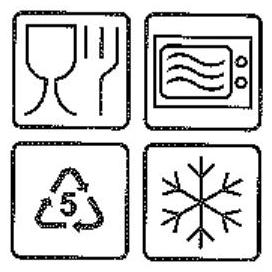
\includegraphics[max width=\textwidth, center]{2025_10_23_80c1361fcdcd395cad8eg-31}\\
vệ sức khoẻ con người.\\
c) Hãy đề xuất một số biện pháp tái sử dụng đồ dùng từ chất dẻo để sử dụng ở gia đình và trường học.\\
9.18. Trong công nghiệp, người ta điều chế PVC từ ethylene (thu được từ dầu mỏ) theo so đồ sau:\\
Ethylene $\xrightarrow[(1)]{\mathrm{Cl}_{2}}$ 1,2-dichloroethane $\xrightarrow[(2)]{500^{\circ} \mathrm{C}}$ vinyl chloride $\xrightarrow[(3)]{\mathfrak{t}^{0}, \mathrm{p}, \mathrm{xt}}$ PVC\\
Giả sử hiệu suất mỗi quá trình (1), (2) và (3) tương ứng là $50 \%$, $65 \%$ và $60 \%$, hãy tính số kg PVC thu được khi dùng $1000 \mathrm{~m}^{3}$ khí ethylène ( $0^{\circ} 25^{\circ} \mathrm{C}$ và 1 bar ).\\
9.19. Trong công nghiệp, để điều chế cao su buna người ta có thể đi từ nguyên liệu khí ethylene thu được từ dầu mỏ theo sơ đồ sau:\\
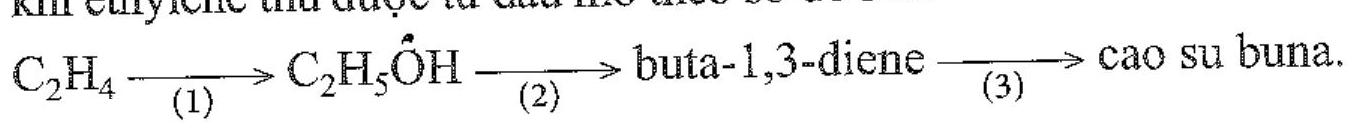
\includegraphics[max width=\textwidth, center]{2025_10_23_80c1361fcdcd395cad8eg-32(1)}

Tính số $\mathrm{m}^{3}$ ethylene ( $0^{\circ} 25^{\circ} \mathrm{C}$ và 1 bar) cần lấy để điều chế được 1 tấn cao su buna theo sơ đồ trên. Giả sử hiệu suất phản ứng của mỗi quá trình (1), (2) và (3) trong sơ đồ trên lần lượt là $65 \%, 50 \%$ và $70 \%$.\\
9.20. Caprolactam được tổng hợp từ cuối thế ki XIX. Hiện nay, nhu cầu sản xuất caprolactam trên thế giới khoảng 10 triệu tấn/năm; $90 \%$ trong đó dùng để tồng hợp tơ capron. Trong công nghiệp, caprolactam được điều chế theo sơ đồ sau:\\
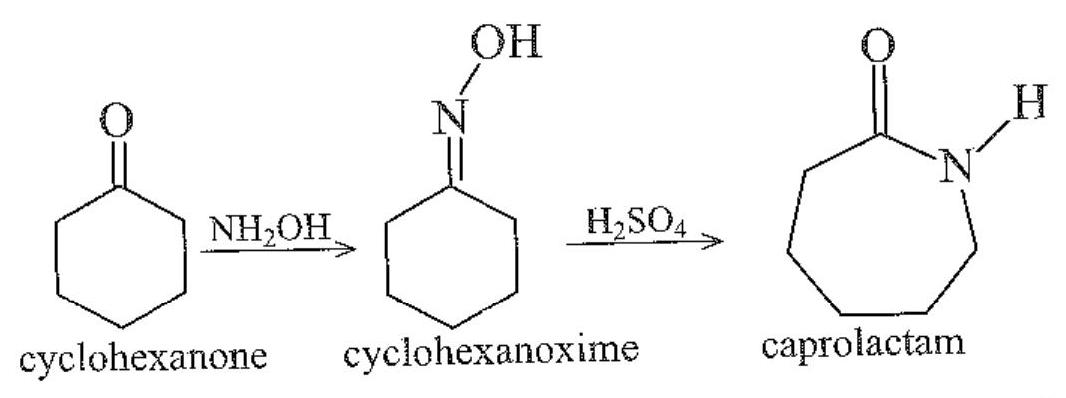
\includegraphics[max width=\textwidth, center]{2025_10_23_80c1361fcdcd395cad8eg-32}

Để sản xuất 10 triệu tấn caprolactam, cần sử dụng bao nhiêu tấn cyclohexanone (giả sử hiệu suất trung bình của cả quá trình trên là $60 \%$ )?

\section*{CHỦDỀ 5 PIN DIÊN YÀ DIỆN PHÂN}
\section*{Bai \\
 10 THẾ DIỆN CỰC CHUẨN CỦA KIM LOAI}
10.1. Điền từ hoặc cụm từ thích hợp vào chỗ trống trong mỗi câu sau.\\
a) Dạng oxi hoá và dạng khử của cùng một ...(1)... kim loại tạo nên cặp ...(2)... của kim loại đó. Dạng oxi hoá là dạng ...(3)... electron và dạng khử là dạng ...(4)... electron.\\
b) Trong phản ứng: $\mathrm{Zn}(s)+\mathrm{Ni}^{2+}(a q) \rightarrow \mathrm{Zn}^{2+}(a q)+\mathrm{Ni}(s)$, chất oxi hoá là ...(1) ..., chất khử là ...(2).... Cặp oxi hoá - khử của nguyên tố kim loại Ni là ...(3)... và cặp oxi hoá - khử của kim loại Zn là ...(4)....\\
10.2. Những phát biểu nào sau đây về phản ứng $\mathrm{Ce}^{4+}+2 \mathrm{I}^{-} \rightarrow \mathrm{I}_{2}+\mathrm{Ce}^{3+}$ là đúng?\\
(a) Phương trình trên đã cân bằng.\\
(b) Chất oxi hoá là $\mathrm{Ce}^{4+}$, chất khử là $\mathrm{I}^{-}$.\\
(c) Cặp oxi hoá - khử của kim loại cerium là $\mathrm{Ce}^{4+} / \mathrm{Ce}$, của iodine là $\mathrm{I}_{2} / 2 \mathrm{I}^{-}$.\\
(d) Phương trình hoá học của phản ứng là; $2 \mathrm{Ce}^{4+}+2 \mathrm{I}^{-} \rightarrow \mathrm{I}_{2}+2 \mathrm{Ce}^{3+}$.\\
10.3. Diền từ hoặc cụm từ thích hợp vào chỗ trống trong mỗi câu sau:\\
a) Thế điện cực chuẩn của cặp oxi hoá - khử càng lớn thì tính oxi hoá của dạng oxi hoá càng ...(1)... và tính khử của dạng khử càng ...(2).... Ngược lại, cặp oxi hoá - khử nào có thế điện cực chuẩn càng ...(3)... thì tính khử của dạng khử càng ...(4)... và tính oxi hoá của dạng oxi hoá càng ...(5)....\\
b) Thế điện cực chuẩn ( $\mathrm{E}^{\circ}$ ) của cặp oxi hoá - khử $\mathrm{Fe}^{2+} / \mathrm{Fe}$ và của cặp $\mathrm{Cu}^{2+} / \mathrm{Cu}$ lần lượt là $-0,440 \mathrm{~V}$ và $0,340 \mathrm{~V}$. Ion $\mathrm{Fe}^{2+}$ có tính ...(1)... yếu hơn ion $\mathrm{Cu}^{2+}$ và Fe có tính ... (2) ... mạnh hơn Cu . Vậy ở điều kiện chuẩn, ... (3) ... có thể khử ...(4)... về ...(5) ... nhưng ion $\mathrm{Fe}^{2+}$ không thể ...(6) ... được Cu .\\
10.4. Dựa vào Bảng 10.1, sách Hoá học 12 , bộ sách Cánh Diều, chỉ ra những phát biểu nào sau đây là kbông đúng?\\
(a) $\mathrm{Cu}^{2+}$ có tính oxi hoá mạnh hơn $\mathrm{Fe}^{3+}$ và Cu có tính khử mạnh hon $\mathrm{Fe}^{2+}$.\\
(b) Zn có tính khử mạnh hơn Pb và $\mathrm{Zn}^{2+}$ có tính oxi hoá yếu hơn $\mathrm{Pb}^{2+}$.\\
(c) Những kim loại có thế điện cực chuần âm đều khử được $\mathrm{H}^{+}$thành $\mathrm{H}_{2}$ và phản úng được trong dung dịch HCl .\\
(d) Trong dãy hoạt động hoá học, những kim loại đứng trước có thế điện cực chuẩn lớn hơn thế điện cực chuẩn của những kim loại đứng sau.\\
(e) Kẽm có thể khử các ion $\mathrm{Fe}^{2+}$ và $\mathrm{Ni}^{2+}$ về kim loại Fe và Ni nhưng không thể khử ion $\mathrm{Al}^{3+}$ về kim loại Al .\\
10.5. Dự đoán những phản ứng nào sau đây có thể tự xảy ra ở điều kiện chuẩn.\\
(a) $\mathrm{Zn}(s)+\mathrm{Sn}^{2+}(a q) \rightarrow$\\
(b) $\mathrm{Ag}^{+}(a q)+\mathrm{Fe}(s) \rightarrow$\\
(c) $\mathrm{Fe}(s)+\mathrm{Mg}^{2+}(a q) \rightarrow$\\
(d) $\mathrm{Au}(s)+\mathrm{Cu}^{2+}(a q) \rightarrow$\\
10.6. Dự đoán hiện tượng nào sau đây sẽ xảy ra khi dùng một chiếc thìa bằng đồng khuấy vào cốc chưa dung dịch aluminium nitrate.\\
A. Chiếc thìa bị phủ một lớp nhôm.\\
B. Một hỗn hợp đồng và nhôm được tạo thành.\\
C. Dung dịch trở nên xanh.\\
D. Không biến đổi hoá học nào xảy ra.\\
10.7. Cho các cặp oxi hoá- khử: $\mathrm{Al}^{3+} / \mathrm{Al} ; \mathrm{Cr}^{3+} / \mathrm{Cr} ; \mathrm{Co}^{2+} / \mathrm{Co} ; \mathrm{Sn}^{4+} / \mathrm{Sn}^{2+}$ và $\mathrm{Cl}_{2}(g) / 2 \mathrm{Cl}^{-}$ với các thế khử chuẩn lần lượt là $-1,676 \mathrm{~V} ;-0,740 \mathrm{~V} ;-0,280 \mathrm{~V} ; 0,150 \mathrm{~V}$ và $1,360 \mathrm{~V}$. Trong các chất tương ứng với các cặp oxi hoá - khử trên, hãy chỉ ra:\\
a) Chất có tính oxi hoá mạnh nhất.\\
b) Chất có khả năng khử $\mathrm{Cr}^{3+}(a q)$ thành $\mathrm{Cr}(s)$ ở điều kiện chuẩn.\\
c) Chất có khả năng khử $\mathrm{Sn}^{4+}(a q)$ thành $\mathrm{Sn}^{2+}(a q)$ nhưng không khử được $\mathrm{Cr}^{3+}(a q)$ thành $\mathrm{Cr}(s)$ ở điều kiện chuẩn.\\
10.8. Cho các thông tin sau:\\
$\mathrm{X}(s)+\mathrm{YSO}_{4}(a q) \rightarrow$ không có phản ứng\\
$\mathrm{Z}(s)+\mathrm{YSO}_{4}(a q) \rightarrow \mathrm{Y}(s)+\mathrm{ZSO}_{4}(a q)$\\
Trong đó, $X, Y, Z$ là các kim loại. Dãy nào sau đây sắp xếp đúng các kim loại theo mức độ hoạt động của chúng?\\
A. $Z>Y>X$.\\
B. $X>Y>Z$.\\
C. $\mathrm{Y}>\mathrm{X}>\mathrm{Z}$.\\
D. $Y>Z>X$.\\
10.9. Những phản ứng nào sau đây không tự xảy ra ở điều kiện chuẩn? Cho $\mathrm{E}_{\mathrm{Mn}^{2+} / \mathrm{Mn}}^{\circ}=-1,180 \mathrm{~V}$.\\
(a) $\mathrm{Mg}^{2+}(a q)+\mathrm{Pb}(s) \rightarrow \mathrm{Pb}^{2+}(a q)+\mathrm{Mg}(s)$\\
(b) $\mathrm{O}_{2}(g)+4 \mathrm{H}^{+}(a q)+2 \mathrm{Zn}(s) \rightarrow 2 \mathrm{H}_{2} \mathrm{O}(l)+2 \mathrm{Zn}^{2+}(a q)$\\
(c) $\mathrm{Ni}(s)+\mathrm{Sn}^{2+}(a q) \rightarrow \mathrm{Ni}^{2+}(a q)+\mathrm{Sn}(s)$\\
(d) $\mathrm{Fe}(s)+\mathrm{Mn}^{2+}(a q) \rightarrow \mathrm{Fe}^{2+}(a q)+\mathrm{Mn}(s)$\\
10.10. Có bốn dung dịch muối không màu $\left(\mathrm{AgNO}_{3}, \mathrm{~Pb}\left(\mathrm{NO}_{3}\right)_{2}, \mathrm{Zn}\left(\mathrm{NO}_{3}\right)_{2}\right.$ và $\left.\mathrm{Ni}\left(\mathrm{NO}_{3}\right)_{2}\right)$ được đựng trong bốn ống nghiệm riêng biệt. Cho thêm vào 4 ống nghiệm này một sợi dây đồng. Sau một thời gian, dung dịch nào chuyển màu xanh? (Các phản ứng đều được thực hiện ở điều kiện chuẩn).\\
A. $\mathrm{AgNO}_{3}$.\\
B. $\mathrm{Pb}\left(\mathrm{NO}_{3}\right)_{2}$.\\
C. $\mathrm{Zn}\left(\mathrm{NO}_{3}\right)_{2}$.\\
D. $\mathrm{Ni}\left(\mathrm{NO}_{3}\right)_{2}$.\\
10.11. Một học sinh thực hiện ba thí nghiệm ở điều kiện chuẩn và quan sát được các hiện tượng sau:\\
(1) Đồng kim loại không phản ứng với dung dịch $\mathrm{Pb}\left(\mathrm{NO}_{3}\right)_{2} 1 \mathrm{M}$.\\
(2) Chì kim loại tan trong dung dịch $\mathrm{AgNO}_{3} 1 \mathrm{M}$ và xuất hiện tinh thể Ag .\\
(3) Bạc kim loại không phản ứng với dung dịch $\mathrm{Cu}\left(\mathrm{NO}_{3}\right)_{2} 1 \mathrm{M}$.

Trật tự nào sau đây thể hiện đúng mức độ khử của ba kim loại?\\
A. $\mathrm{Cu}>\mathrm{Pb}>\mathrm{Ag}$.\\
B. $\mathrm{Pb}>\mathrm{Cu}>\mathrm{Ag}$.\\
C. $\mathrm{Cu}>\mathrm{Ag}>\mathrm{Pb}$.\\
D. $\mathrm{Pb}>\mathrm{Ag}>\mathrm{Cu}$.\\
10.12*. Những kim loại nào sau đây có thể được dùng để bảo vệ đường ống sắt khỏi bị gi?\\
(a) Cr.\\
(b) Ag .\\
(c) Cu.\\
(d) Mn.\\
(e) Zn .\\
10.13. Những phản ứng hoá học sau đây xảy ra trong dung dịch:\\
(1) $2 \mathrm{Al}(s)+3 \mathrm{Cu}^{2+}(a q) \rightarrow 2 \mathrm{Al}^{3+}(a q)+3 \mathrm{Cu}(s)$\\
(2) $2 \mathrm{Al}(s)+3 \mathrm{Fe}^{2+}(a q) \rightarrow 2 \mathrm{Al}^{3+}(a q)+3 \mathrm{Fe}(s)$\\
(3) $\mathrm{Pb}^{2+}(a q)+\mathrm{Fe}(s) \rightarrow \mathrm{Fe}^{2+}(a q)+\mathrm{Pb}(s)$\\
(4) $\mathrm{Fe}(s)+\mathrm{Cu}^{2+}(a q) \rightarrow \mathrm{Fe}^{2+}(a q)+\mathrm{Cu}(s)$\\
(5) $2 \mathrm{Al}(s)+3 \mathrm{~Pb}^{2+}(a q) \rightarrow 2 \mathrm{Al}^{3+}(a q)+3 \mathrm{~Pb}(s)$\\
(6) $\mathrm{Pb}(s)+\mathrm{Cu}^{2+}(a q) \rightarrow \mathrm{Pb}^{2+}(a q)+\mathrm{Cu}(s)$

Sắp xếp các kim loại tham gia các phản ứng trên theo thứ tự giảm dần về khả năng dễ bị oxi hoá.\\
10.14*. Trong phòng thí nghiệm, một học sinh nhúng thanh đồng có khối lượng $12,340 \mathrm{~g}$ vào 255 mL dung dịch $\mathrm{AgNO}_{3} 0,125 \mathrm{M}$. Bằng quan sát, học sinh đó đã khẳng định có phản ứng xảy ra.\\
a) Vì sao học sinh đó lại khẳng định có phản ứng xảy ra chỉ bằng việc quan sát?\\
b) Viết và cân bằng phương trình hoá học của phản ứng.\\
c) Viết các cặp oxi hoá - khử tham gia phản ứng và chỉ rõ tác nhân oxi hoá và tác nhân khử.\\
d) Khi phản ứng kết thúc, hãy xác định khối lượng của thanh đồng, nếu giả thiết rằng toàn bộ lượng Ag giải phóng đều bám vào thanh đồng.\\
10.15*. Trong phòng thí nghiệm, một bạn học sinh khi nhỏ từ từ dung dịch thuốc tím vào dung dịch $\mathrm{Fe}^{2+}$ trong môi trường acid đã quan sát thấy thuốc tím mất màu và dung dịch dần chuyền từ không màu sang màu vàng nhạt. Phản ứng được thực hiện ở điều kiện chuẩn.\\
a) Giải thích hiện tượng bạn học sinh quan sát được.\\
b) Viết các cặp oxi hoá - khử của hai nguyên tố Mn vẩ Fe liên quan đến phản ứng trong quá trình trên và so sánh thế điện cực chuẩn của hai cặp oxi hoá - khử này.\\
c) Viết phương trình chuyển hoá giữa dạng oxi hoá và dạng khử của mỗi cặp oxi hoá - khử và phương trình hoá học khi phản ứng xảy ra.

\section*{BBAI \\
 11 NGUỒN DIỆN HOÁ HOC}
11.1. Điền từ hoặc cụm từ thích hợp vào chỗ trống trong các câu sau.\\
a) Nguồn điện ...(1) ... là một loại nguồn điện được tạo ra bằng cách sử dụng các phản ứng hoá học để tạo ra ... (2)....\\
b) Phản ứng trong pin điện hoá diễn ra trong điều kiện ...(1)... (tương ứng với hai điện cực) ở hai khu vực khác nhau được nối với nhau bởi dây dẫn. Khi đó, dòng electron được chuyển gián tiếp từ ...(2)... sang chất oxi hoá thông qua dây dẫn điện, ta có pin ...(3)....\\
11.2. Những phát biểu nào sau đây là không đúng?\\
(a) Một ưu điểm của acquy là tái sử dụng được nhiều lần.\\
(b) Phản ứng xảy ra trong acquy cũng giống như phản ứng xảy ra trong pin. Galvani nhưng có thể đảo ngược.\\
(c) Acquy không gây ô nhiễm môi trường.\\
(d) Acquy là nguồn điện hoá học có thể hoạt động liên tục.\\
11.3. Nhận định nào sau đây về pin nhiên liệu là không đúng?\\
A. Khác với acquy, chất phản ứng của pin nhiên liệu phải được cung cấp liên tục từ nguồn bên ngoài.\\
B. Pin nhiên liệu tạo ra điện năng nhờ năng lượng mặt trời.\\
C. Pin nhiên liệu biến đồi trực tiếp năng lượng hoá học thành điện năng.\\
D. Một trong những hạn chế của pin nhiên liệu là sự lưu trữ nhiên liệu.\\
E. Khi sử dụng, pin nhiên liệu không gây ô nhiễm môi trường.\\
11.4. Trong pin Galvani, thành phần nào dưới đây không phải là một phần cấu tạo nhất định phải có trong pin?\\
A. Điện cực dương.\\
B. Điện cực âm.\\
C. Cầu muối.\\
D. Dây dẫn điện.\\
11.5. Khi nói về cầu muối trong pin Galvani, mỗi phát biểu sau đây là đúng hay sai?\\
(a) Cầu muối có tác dụng trung hoà điện tích của dung dịch trong pin.\\
(b) Cầu muối cho phép dòng điện chạy qua.\\
(c) Dòng điện chạy qua cầu muối là dòng electron.\\
(d) Muối trong cầu muối luôn cố định là KCl .\\
11.6. Bảng dưới đây mô tả các thành phần của pin Galvani và vai trò của từng thành phần. Hoàn thiện những thông tin còn thiếu trong bảng sau.

\begin{center}
\begin{tabular}{|l|l|l|}
\hline
Thành phân & Vai trò & Vi du \\
\hline
? & Nơi diễn ra phản ứng khử & ? \\
\hline
Diện cực âm (anode) & ? & Zn \\
\hline
Dung dịch chứa ion của điện cực âm & Môi trường cho phản ứng oxi hoá & ? \\
\hline
? & Môi trường cho phản ứng khử & Dung dịch $\mathrm{AgNO}_{3}$ \\
\hline
? & ? & $\mathrm{KNO}_{3}$ \\
\hline
\end{tabular}
\end{center}

11.7. Một pin Galvani được cấu tạo bởi hai cặp oxi hoá - khử sau:\\
(1) $\mathrm{Ag}^{+}+\mathrm{e} \rightarrow \mathrm{Ag}$

$$
\mathrm{E}_{\mathrm{Ag}^{+} / \mathrm{Ag}}^{0}=0,799 \mathrm{~V}
$$

(2) $\mathrm{Ni}^{2+}+2 \mathrm{e} \rightarrow \mathrm{Ni}$

$$
\mathrm{E}_{\mathrm{Ni}^{2+} / \mathrm{Ni}}^{\circ}=-0,257 \mathrm{~V}
$$

Khi pin làm việc ở điều kiện chuẩn, nhận định nào sau đây là đúng?\\
A. Ag được tạo ra ở cực dương, Ni được tạo ra ở cực âm.\\
B. Ag được tạo ra ở cực dương, $\mathrm{Ni}^{2+}$ được tạo ra ở cực âm.\\
C. $\mathrm{Ag}^{+}$được tạo ra ở cực âm và Ni được tạo ra ở cực dương.\\
D. $\mathrm{Ag}^{+}$được tạo ra ở cực âm và $\mathrm{Ni}^{2+}$ được tạo ra ở cực dương.\\
11.8. Sức điện động chuẩn của pin Galvani được tính như thế nào?\\
A. Bằng hiệu của thế điện cực chuẩn tương ứng của điện cực dương và điện cực âm.\\
B. Bằng tổng của thế điện cực chuẩn tương ứng của điện cực dương và điện cực âm.\\
C. Bằng tích của thế điện cực chuẩn tương ứng của điện cực dương và điện cực âm.\\
D. Bằng thương của thế điện cực chuẩn tương ứng của điện cực dương và điện cực âm.\\
11.9. Nếu thế khử chuẩn của điện cực dương là $0,80 \mathrm{~V}$ và thế khử chuẩn của điện cực âm là $-0,76 \mathrm{~V}$ thì sức điện động chuẩn của pin-Gálvani tạo từ hai điện cực trên là bao nhiêu?\\
A. $1,56 \mathrm{~V}$.\\
B. $-1,56 \mathrm{~V}$.\\
C. $0,04 \mathrm{~V}$.\\
D. $-0,04 \mathrm{~V}$.\\
11.10. Khi nói về pin Galyani, mỗi phát biểu sau đây là đúng hay sai?\\
(a) Sức điện động chuẩn của pin Galvani có thể mang giá trị âm.\\
(b) Khi pin Galvani hoạt động, không có phản úng hoá học diễn ra.\\
(c) Pin Galvani cung cấp nguồn điện hoá học.\\
(d) Sức điện động chuẩn của pin Galvani chỉ có thể mang giá trị dương.\\
11.11. Khi làm việc, acquy là thiết bị sinh ra dòng điện hoạt động theo nguyên tắc giống như pin Galvani (quá trình acquy phóng điện). Nhưng khác với pin Galvani, acquy có thể tái sử dụng nhờ dùng một dòng điện bên ngoài "ép" phản úng điện hoá xảy ra khi acquy làm việc theo chiều ngược lại (quá trình sạc điện).\\
Cho 4 phản ứng sau:\\
(1) $\mathrm{Pb}+\mathrm{SO}_{4}^{2-} \rightarrow \mathrm{PbSO}_{4}+2 \mathrm{e}$\\
(2) $\mathrm{PbO}_{2}+\mathrm{SO}_{4}^{2-}+4 \mathrm{H}^{+}+2 \mathrm{e} \rightarrow \mathrm{PbSO}_{4}+2 \mathrm{H}_{2} \mathrm{O}$\\
(3) $\mathrm{Pb}+\mathrm{PbO}_{2}+2 \mathrm{SO}_{4}^{2-}+4 \mathrm{H}^{+} \rightarrow 2 \mathrm{PbSO}_{4}+2 \mathrm{H}_{2} \mathrm{O}$\\
(4) $2 \mathrm{PbSO}_{4}+2 \mathrm{H}_{2} \mathrm{O} \rightarrow \mathrm{Pb}+\mathrm{PbO}_{2}+2 \mathrm{SO}_{4}^{2-}+4 \mathrm{H}^{+}$

Hãy chỉ ra:\\
a) Phản ứng điện hoá xảy ra ở cực dương khi acquy làm việc.\\
b) Phản ứng điện hoá xảy ra ở cực âm khi acquy làm việc.\\
c) Phản ứng điện hoá tổng quát xảy ra khi acquy làm việc.\\
d) Phản ứng xảy ra khi acquy sạc điện.\\
11.12. Xét pin Galvani hoạt động với phương trình tương ứng như sau:

$$
\mathrm{Zn}+\mathrm{HgO} \rightarrow \mathrm{ZnO}+\mathrm{Hg}
$$

Quá trình nào sau đây xuất hiện ở anode?\\
A. $\mathrm{HgO}+2 \mathrm{e} \rightarrow \mathrm{Hg}+\mathrm{O}^{2-}$\\
B. $\mathrm{Zn}^{2+}+2 \mathrm{e} \rightarrow \mathrm{Zn}$\\
C. $\mathrm{Zn} \rightarrow \mathrm{Zn}^{2+}+2 \mathrm{e}$\\
D. $\mathrm{Hg}+\mathrm{O}^{2-} \rightarrow \mathrm{HgO}+2 \mathrm{e}$\\
11.13. Xét pin Galvani hoạt động với phương trình tương ứng:

$$
\mathrm{Zn}(s)+\mathrm{Cu}^{2+}(a q) \rightarrow \mathrm{Cu}(s)+\mathrm{Zn}^{2+}(a q)
$$

Những phương án nào sau đây là đúng?\\
(a) Điện cực đồng giảm khối lượng và điện cực đồng là cực âm.\\
(b) Điện cực đồng tăng khối lượng và điện cực đồng là cực dương.\\
(c) Điện cực kẽm giảm khối lượng và điện cực kẽm là cực âm.\\
(d) Điện cực kẽm tăng khối lượng và điện cực kẽm là cực dương.\\
11.14*. Cho một pin Galvani với điện cực Zn và Cu có sức điện động chuẩn là $1,34 \mathrm{~V}$. Sử dụng pin này để thắp sáng một bóng đèn nhỏ với cường độ dòng điện chạy qua là $\mathrm{I}=0,02 \mathrm{~A}$. Nếu điện cực kẽm hao mòn $0,1 \mathrm{~mol}$ do pin phóng điện thì thời gian tối đa mà pin thắp sáng được bóng đèn là bao nhiêu giờ? Cho biết các công thức:\\
$\mathrm{Q}=\mathrm{n} . \mathrm{F}=\mathrm{I} . \mathrm{t}$, trong đó: Q là điện lượng $(\mathrm{C}), \mathrm{n}$ là số mol electron đi qua dây dẫn, I là cường độ dòng điện (A), t là thời gian (giây), F là hằng số Faraday ( $96500 \mathrm{C} \mathrm{mol}^{-1}$ ).\\
11.15. Trong pin nhiên liệu hydrogen, $\mathrm{H}_{2}$ có vai trò tương tự như kim loại mạnh hơn trong pin Galvani. Phản ứng nào sau đây diễn ra ở điện cực dương khi pin nhiên liệu hydrogen hoạt động?\\
A. $2 \mathrm{H}_{2}+\mathrm{O}_{2} \rightarrow 2 \mathrm{H}_{2} \mathrm{O}$\\
B. $\mathrm{H}_{2} \rightarrow 2 \mathrm{H}^{+}+2 \mathrm{e}$\\
C. $\mathrm{O}_{2}+4 \mathrm{H}^{+}+4 \mathrm{e} \rightarrow 2 \mathrm{H}_{2} \mathrm{O}$\\
D. $2 \mathrm{H}^{+}+2 \mathrm{e} \rightarrow \mathrm{H}_{2}$\\
11.16. Những phát biểu nào sau đây về pin nhiên liệu là đúng?\\
(a) Cho hiệu suất chuyển hoá điện năng cao.\\
(b) Biến đổi trực tiếp hoá năng thành điện năng nhờ quá trình oxi hoá trực tiếp nhiên liệu.\\
(c) Gây ô nhiễm môi trường khi hoạt động.\\
(d) Hoạt động liên tục không nghỉ nếu nhiên liệu được cung cấp liên tục.

\section*{Bell \\
 12 DIỆN PHÂN}
12.1. Điền từ hoặc cụm từ thích hợp vào chỗ trống trong các câu sau:\\
a) Điện phân là quá trình ...(1)... xảy ra trên bề mặt các điện cực dưới tác dụng của ...(2)... đi qua dung dịch chất điện li hoặc chất điện li nóng chảy.\\
b) Trong quá trình điện phân, ở cực âm, chất nào có tính oxi hoá ... (1) ... được ưu tiên điện phân trước. Ở cực dương, chất nào có tính khử ...(2)... được ưu tiên điện phân trước. Điện phân có nhiều ứng dụng quan trọng trong thực tiễn, như sản xuất kim loại ...(3)..., mạ điện, ...(4)....\\
12.2. Phát biểu nào sau đây về thứ tự điện phân trong dung dịch của các ion kim loại ở điện cực là đúng?\\
A. Ion kim loại ứng với thế điện cực chuẩn dương hơn sẽ được điện phân trước ở cực âm.\\
B. Ion kim loại ứng với thế điện cực chuẩn âm hơn sẽ được điện phân trước ở cực âm.\\
C. Ion kim loại ứng với thế điện cực chuẩn dương hơn sẽ được điện phân trước ở cực dương.\\
D. Ion kim loại ứng với thế điện cực chuẩn âm hơn sẽ được điện phân trước ở cực dương.\\
12.3. Vẽ một bình điện phân trong đó $\mathrm{Mn}^{2+}$ bị khử thành Mn và Sn bị oxi hoá thành $\mathrm{Sn}^{2+}$. Ghi nhãn cho cực dương và cực âm, chỉ ra hướng chuyển động của các electron và viết phương trình hoá học xảy ra ở mỗi điện cực. Điện áp tối thiểu cần thiết để xảy ra sự điện phân là bao nhiêu? Biết $\mathrm{E}_{\mathrm{Mn}^{2} / \mathrm{Mn}}^{\circ}=-1,18 \mathrm{~V}$.\\
12.4. Khi điện phân dung địch NaCl có màng ngăn, các chất được tạo ra ở anode (cực dương) và cathode (cực âm) lần lượt là\\
A. $\mathrm{Cl}_{2}$ và $\mathrm{NaOH}, \mathrm{H}_{2}$.\\
B. Na và $\mathrm{Cl}_{2}$.\\
C. $\mathrm{Cl}_{2}$ và Na .\\
D. NaOH và $\mathrm{H}_{2}$.\\
12.5. Điện phân dung dịch hỗn hợp gồm HCl và $\mathrm{CuSO}_{4}$ có cùng nồng độ. Các chất được tạo ra đầu tiên ở anode (cực dương) và ở cathode (cực âm) lần lượt là:\\
A. $\mathrm{Cl}_{2}$ và $\mathrm{H}_{2}$.\\
B. $\mathrm{Cl}_{2}$ và Cu .\\
C. $\mathrm{O}_{2}$ và Cu .\\
D. $\mathrm{O}_{2}$ và $\mathrm{H}_{2}$.\\
12.6. Điện phân dung dịch NaCl có màng ngăn với cường độ dòng điện 10 A trong 2 giờ. Tính khối lượng dung dịch giảm sau khi điện phân, giả thiết chỉ có phản ứng điện phân dung dịch NaCl , bỏ qua lượng nước bay hơi. Cho biết các công thức:\\
$\mathrm{Q}=\mathrm{n} \cdot \mathrm{F}=\mathrm{I} \cdot \mathrm{t}$, trong đó: Q là điện lượng $(\mathrm{C}), \mathrm{n}$ là số mol electron đi qua dây dẫn, I là cường độ dòng điện ( A ), t là thời gian (giây), F là hằng số Faraday ( $96500 \mathrm{C} \mathrm{mol}^{-1}$ ).\\
12.7. Một loại quặng nhôm có chứa $40 \%$ khối lượng Al.\\
a) Nhôm trong loại quặng trên ở dạng $\mathrm{Al}_{2} \mathrm{O}_{3}$, hỏi quặng trên chứa bao nhiêu phần trăm tạp chất.\\
b) Để điện phân toàn bộ lượng $\mathrm{Al}_{2} \mathrm{O}_{3}$ nóng chảy thu được từ 1000 kg loại quặng trên bởi dòng điện một chiều có cường độ 10000 A thì về lí thuyết cần bao nhiêu giờ điện phân liên tục? Cho biết số mol electron n đi qua dây dẫn được tính theo công thức $\mathrm{n}=(\mathrm{I} . \mathrm{t}) / \mathrm{F}$.\\
Trong đó, I là cường độ dòng điện ( A ), t là thời gian ( s ), F là số Faraday ( $96500 \mathrm{C} \mathrm{mol}^{-1}$ ).\\
12.8. Khi điện phân dung dịch $\mathrm{CuSO}_{4}$, ion nào sẽ điện phân đầu tiên ở cathode?\\
A. $\mathrm{Cu}^{2+}$.\\
B. $\mathrm{H}^{+}$(của nước).\\
C. $\mathrm{SO}_{4}^{2-}$.\\
D. $\mathrm{OH}^{-}$(của nước).\\
12.9. Dựa vào các giá trị thế điện cực chuần sau, hãy giải thích vì sao khi điện phân dung dịch NaCl có màng ngăn lại không thu được Na kim loại. Viết phương trình phản ứng điện phân đầu tiên xảy ra ở cathode.

\begin{center}
\begin{tabular}{|l|l|l|}
\hline
Cặp oxi hoá - khử & $2 \mathrm{H}_{2} \mathrm{O} / \mathrm{H}_{2}+2 \mathrm{OH}^{-}$ & $\mathrm{Na}^{+} / \mathrm{Na}$ \\
\hline
Thế điện cực chuẩn (V) & $-0,83$ & $-2,71$ \\
\hline
\end{tabular}
\end{center}

12.10. Trong một dung dịch có đồng thời các ion kim loại: $\mathrm{Fe}^{2+}, \mathrm{Cu}^{2+}, \mathrm{Ag}^{+}, \mathrm{Zn}^{2+}$. Hãy lập luận để chỉ ra thứ tự điện phân của các ion ở cathode.\\
12.11*. Cần mạ một lớp Ag lên một mặt của một chiếc đĩa tròn có bán kính 12 cm . Với độ dày lớp mạ là $0,01 \mathrm{~mm}$, nếu được cung cấp nguồn điện một chiều có cường độ dòng điện $\mathrm{I}=2 \mathrm{~A}$ trong thời gian $\mathrm{t}=3$ giờ thì có đủ để mạ theo yêu cầu trên không? Biết rằng khối lượng riêng của Ag là $10,5 \mathrm{~g} \mathrm{~cm}^{-3}$, hiệu suất điện phân là $100 \%$.

\section*{CHỦDỀ 6 DAI CƯƠNG VỀ KIMLOAI}
\section*{Pail \\
 13 CẤU TAO VÀ TÍNH CHẤT VÂT LÍ CỦA KIM LOAI}
13.1. Cho các phát biểu sau về tinh thể kim loại M :\\
(1) Trong tinh thể kim loại M có các cation $\mathrm{M}^{\mathrm{n}+}$ và các electron hoá trị tự do.\\
(2) Trong tinh thể kim loại M có các electron hoá trị tự do chuyển động.\\
(3) Các cation $\mathrm{M}^{\mathrm{p}+}$ chuyển động tự do trong mạng tinh thể kim loại.\\
(4) Lực hút giữa cation $\mathrm{M}^{\mathrm{n}+}$ và electron hoá trị tự do trong tinh thể kim loại M phụ thuộc vào độ âm điện của kim loại M .\\
(5) Tinh thể kim loại M trung hoà về điện.\\
(6) Trong tinh thể kim loại M , các cation $\mathrm{M}^{\mathrm{n}+}$ và electron hoá trị tự do được phân bố theo trật tự nhất định.\\
Số phát biểu đúng là\\
A. 2 .\\
B. 3 .\\
C. 4 .\\
D. 1 .\\
13.2. Phát biểu nào sau đây về liên kết kim loại là đúng?\\
A. Liên kết kim loại là liên kết được hình thành từ lực hút tĩnh điện giữa các cation kim loại và các electron hoá trị tự do. Vì vậy, liên kết kim loại cũng chính là liên kết ion.\\
B. Liên kết kim loại được hình thành do giữa các nguyên tử kim loại có sự dùng chung các electron hoá trị tự do. Vì vậy, liên kết kim loại cũng chính là liên kết cộng hoá trị.\\
C. Liên kết kim loại là liên kết được hình thành từ lực hút tĩnh điện giữa các cation kim loại và các electron hoá trị tự do trong tinh thể kim loại.\\
D. Liên kết kim loại là liên kết được hình thành do sự xen phủ các orbital chứa electron hoá trị tự do của các nguyên tử kim loại.\\
13.3. Những phát biểu nào sau đây là đúng?\\
(a) Ở điều kiện thường, tất cả các kim loại đều tồn tại ở thể rắn và có cấu tạo tinh thể.\\
(b) Các cation kim loại và nguyên tử kim loại được sắp xếp trật tự trong tinh thể kim loại.\\
(c) Electron hoá trị của nguyên tử kim loại chịu lực hút yếu của hạt nhân nguyên tử.\\
(d) Giống như liên kết ion, liện kết kim loại cũng được hình thành từ tương tác tĩnh điện.\\
(e) Các electron hoá trị tự do di chuyển trong cấu trúc tinh thể kim loại tạo ra dòng điện.\\
13.4. Nhóm những kim loại có độ dẫn điện tốt nhất là\\
A. $\mathrm{Ag}, \mathrm{Cu}, \mathrm{Au}$.\\
B. $\mathrm{Cu}, \mathrm{Al}, \mathrm{Hg}$.\\
C. $\mathrm{Li}, \mathrm{Na}, \mathrm{K}$.\\
D. $\mathrm{Fe}, \mathrm{Cu}, \mathrm{Zn}$.\\
13.5. Những phát biểu nào sau đây là không đúng?\\
(a) Chromium thường được mạ bên ngoài một số đồ vật là do kim loại này cứng và có khả năng chống mài mòn tốt.\\
(b) Nhôm được sử dụng nhiều trong sản xuất máy bay là do nhôm có ánh kim phản xạ các tia cực tím từ mặt trời.\\
(c) Bạc được dùng phổ biến làm dây dẫn điện vì là kim loại có độ dẫn điện tốt nhất.\\
(d) Bạc được dùng để tráng gương là do bạc là kim loại dẫn nhiệt rất tốt.\\
13.6. Hoàn thành bảng sau:

\begin{center}
\begin{tabular}{|l|l|l|}
\hline
Tinh chát vạt lí & Ví du úng dung turong úng & Ví du ki hiêu hoá học cua kim loai phù hop \\
\hline
Nhiệt độ nóng chảy rất cao & Dây tóc bóng đèn & $\ldots$ (?) $\ldots$ \\
\hline
$\ldots$ (?) $\ldots$ & Bảo vệ bề mặt, chống mài mòn & $\ldots$ (?) $\ldots$ \\
\hline
Khối lượng riêng nhỏ & $\ldots$ (?) $\ldots$ & . . .(?)... \\
\hline
Độ dẫn điện cao & . . .(?)... & $\ldots$ (?) $\ldots$ \\
\hline
$\ldots$ (?) $\ldots$ & Dây chảy của cầu chì & $\ldots$ (?) $\ldots$ \\
\hline
$\ldots$ (?) $\ldots$ & Đồ trang sức & $\ldots$ (?) $\ldots$ \\
\hline
\end{tabular}
\end{center}

13.7. Mỗi phát biểu sau đây là đúng hay sai?\\
(a) Kim loại dẻo là nhờ lực hút tĩnh điện giữa các cation kim loại và các electron hoá trị tự do.\\
(b) Ở điều kiện thường, thuỷ ngân không có cấu trúc tinh thể nên không dẫn điện.\\
(c) Nhôm là kim loại vừa dẫn điện tốt vừa dẫn nhiệt tốt.\\
(d) Kim loại có vẻ sáng lấp lánh là do các cation trong tinh thể phản xạ phần lớn các tia sáng nhìn thấy được.\\
13.8. Nhờ có hàm lượng lớn trong vỏ Trái Đất nên một số kim loại được sử dụng làm kim loại cơ bản trong các hợp kim, đó là\\
A. sắt, nhôm và magnesium.\\
B. sắt, kẽm và calcium.\\
C. nhôm, magnesium và sodium.\\
D. sắt, nhôm và thiếc.\\
13.9. Dựa vào tính chất vật lí của kim loại, tìm hiểu và giải thích vì sao dây dẫn điện gia dụng thường được làm bằng đồng; dây dẫn điện cao thế lại được làm bằng nhôm; vật dẫn trong các linh kiện điện tử lại được làm bằng vàng; trong khi đó bạc là kim loại dẫn điện tốt nhất lại ít được sử dụng?

\section*{Bol \\
 14 TÍNH CHẤT HOÁ HỌC CỦA KIM LOAI}
14.1. Những phát biểu nào sau đây là đúng?\\
(a) Tính chất hoá học đặc trưng của kim loại là tính khử.\\
(b) Kim loại càng hoạt động hoá học thì tính khử càng mạnh.\\
(c) Những kim loại kém hoạt động hoá học (tro) như vàng, platinum không thể hiện tính khử.\\
(d) Kim loại bạc có tính khử yếu trong khi cation $\mathrm{Ag}^{+}$có tính oxi hoá mạnh.\\
(e) Kim loại mạnh có thể khử các kim loại yếu hơn trong hợp kim.\\
14.2. Những phát biểu nào sau đây là đúng?\\
(a) Thông thường, kim loại M hoạt động càng mạnh thì giá trị thế điện cực chuẩn của cặp oxi hoá - khử $\mathrm{M}^{\mathrm{n}+} / \mathrm{M}$ càng âm.\\
(b) Kim loại M càng kém hoạt động thì giá trị thế điện cực chuẩn của cặp oxi hoá - khử $\mathrm{M}^{\mathrm{n}+} / \mathrm{M}$ càng dương.\\
(c) Trong cặp oxi hoá - khử $2 \mathrm{H}_{2} \mathrm{O} /\left(\mathrm{H}_{2}+2 \mathrm{OH}^{-}\right)$thì $\mathrm{H}_{2} \mathrm{O}$ là dạng khư, $\mathrm{H}_{2}$ là dạng oxi hoá.\\
(d) Magnesium là kim loại có độ hoạt động hoá học mạnh hon nhôm (aluminium), giá trị thế điện cực chuẩn của cặp $\mathrm{Mg}^{2+} / \mathrm{Mg}$ âm hơn giá trị thế điện cực chuẩn của cặp $\mathrm{Al}^{3+} / \mathrm{Al}$.\\
14.3. Dựa vào giá trị thế điện cực chuẩn của các cặp oxi hoá - khử liên quan, hãy cho biết trường hợp nào sau đây không có phản ứng hoá học xảy ra ở điều kiện chuẩn. Viết phương trình hoá học của các phản ứng xảy ra.\\
a) Cho kẽm (zinc) vào dung dịch tin(II) sulfate.\\
b) Cho sắt (iron) vào dung dịch magnesium nitrate.\\
c) Cho chì (lead) vào dung dịch hydrochloric acid.\\
d) Cho chì vào dung dịch zinc chloride.\\
e) Cho đồng (copper) vào nước.\\
14.4. Ở môi trường trung tính, quá trình $2 \mathrm{H}_{2} \mathrm{O}+2 \mathrm{e} \rightarrow \mathrm{H}_{2}+2 \mathrm{OH}^{-}$có giá trị $\mathrm{E}_{2 \mathrm{H}_{2} \mathrm{O} / 2 \mathrm{OH}^{-}+\mathrm{H}_{2}}^{\mathrm{O}}=-0,413 \mathrm{~V}$. Những phát biểu nào sau đây là không đúng?\\
(a) Những kim loại M có thế điện cực chuẩn $\mathrm{E}_{\mathrm{M}^{+} / \mathrm{M}}^{\mathrm{o}}<-0,413 \mathrm{~V}$ đều khử được nước ở điều kiện thường.\\
(b) Sodium khử được nước theo phương trình hoá học: $2 \mathrm{Na}+2 \mathrm{H}_{2} \mathrm{O} \rightarrow 2 \mathrm{NaOH}+\mathrm{H}_{2}$ nên $\mathrm{E}_{\mathrm{Na}^{+} / \mathrm{Na}}^{\mathrm{o}}<-0,413 \mathrm{~V}$.\\
(c) Nước đóng vai trò là chất khử khi phản ứng với kim loại M (như $\mathrm{Na}, \mathrm{K}$ ) có thế điện cực chuẩn $\mathrm{E}_{\mathrm{M}^{+} / \mathrm{M}}^{0}<-0,413 \mathrm{~V}$.\\
(d) Khí hydrogen là sản phẩm khử của nước khi nước phản ứng với kim loại mạnh như Na, K.\\
14.5. Thả một đinh sắt nặng $\mathrm{m}_{1}$ gam đã được đánh sạch bề mặt vào cốc chứa dung dịch copper(II) sulfate màu xanh. Sau một thời gian thấy toàn bộ lượng đồng sinh ra đã bám vào "đinh sắt" (thực chất là phần đinh sắt chưa phản ứng). Lấy "đỉnh sắt" ra khỏi cốc dung dịch, sấy khô, đem cân được $m_{2}$ gam.\\
Mỗi phát biểu sau đây là đúng hay sai?\\
(a) Phản ứng diễn ra là: $2 \mathrm{Fe}(s)+3 \mathrm{Cu}^{2+}(a q) \rightarrow 2 \mathrm{Fe}^{3+}(a q)+3 \mathrm{Cu}(s)$\\
(b) Màu xanh của dung dịch copper(II) sulfate nhạt dần.\\
(c) So sánh, thu được kết quả $\mathrm{m}_{2}<\mathrm{m}_{1}$.\\
(d) Nếu thay đinh sắt ban đầu bằng thanh kẽm thì màu xanh của dung dịch không thay đồi.\\
14.6. Cho một ít bột nhôm vào muỗng đốt hoá chất rồi đốt trên ngọn lửa đèn cồn. Khi một phần bột nhôm trong muỗng cháy đỏ thì đưa nhanh muỗng vào bình chứa oxygen du. Bột nhôm cháy nhanh và phát ra ánh sáng màu trắng rất mạnh, tạo thành hợp chất $\mathbf{A}$.\\
Mỗi phát biểu dưới đây đúng hay sai?\\
(a) Nhôm bị khử tạo thành hợp chất $\mathbf{A}$.\\
(b) Số oxi hoá của nhôm trong hợp chất $\mathbf{A}$ là +3 .\\
(c) Biến thiên enthalpy chuẩn của phản ứng giữa nhôm và oxygen có giá trị âm ( $\triangle_{\mathrm{r}} \mathrm{H}_{298}^{\mathrm{o}}<0$ ).\\
(d) Phản ứng trên liên quan đến 2 cặp oxi hoá - khử là $\mathrm{Al}^{3+} / \mathrm{Al}$ và $\mathrm{O}_{2} / 2 \mathrm{O}^{2-}$.\\
14.7. Cho 3 thí nghiệm sau:

\begin{itemize}
  \item Thí nghiệm 1: Cho một mẩu sodium vào nước đã thêm vài giọt dung dịch phenolphthalein.
  \item Thí nghiệm 2: Cho một mẩu kẽm vào dung dịch hydrochloric acid loãng.
  \item Thí nghiệm 3: Cho một mẩu đồng vào dung dịch sulfuric acid đặc.
\end{itemize}

Mỗi phát biểu dưới đây là đúng hay sai?\\
(a) Các kim loại bị oxi hoá trong cả ba thí nghiệm trên.\\
(b) Cả ba dung dịch đều đổi màu trong quá trình phản ứng,\\
(c) Thí nghiệm 3 có sinh ra khí $\mathbb{Z}$. Tỉ khối hơi của khí $\mathbb{Z}$ so với khí $\mathbb{X}$ thoát ra ở thí nghiệm 1 là 32 .\\
(d) Tổng hệ số tối giản của các chất trong phương trình hoá học ở thí nghiệm 3 là 6 .\\
14.8. Dựa vào giá trị thế điện cực chuẩn của các cặp oxi hoá - khử $\mathrm{M}^{\mathrm{n}+} / \mathrm{M}$ với M là $\mathrm{Cu}, \mathrm{Hg}, \mathrm{K}$ và Zn , hãy:\\
a) Sắp xếp các kim loại theo chiều tính khử tăng dần.\\
b) Sắp xếp các cation $\mathrm{Cu}^{2+}, \mathrm{Hg}^{2+}, \mathrm{K}^{+}, \mathrm{Zn}^{2+}$ theo chiều tính oxi hoá tăng dần.\\
c) Cho biết kim loại nào có khả năng phản úng với dung dịch hydrochloric acid ở điều kiện thường.\\
14.9. Nhóm những kim loại nào sau đây không phản ứng vói dung dịch sulfuric acid đặc, nguội?\\
A. Fe, Al, Ag.\\
B. $\mathrm{Fe}, \mathrm{Au}, \mathrm{Cr}$.\\
C. $\mathrm{Fe}, \mathrm{Al}, \mathrm{Zn}$.\\
D. Al, Cr, Zn.\\
14.10. Trường hợp nào sau đây có xảy ra phản ứng hoá học? Giải thích và viết phương trình hoá học (nếu có).\\
a) Kim loại đồng nhúng trong dung dịch zinc sulfate.\\
b) Kim loại kẽm nhúng trong dung dịch silver nitrate.\\
c) Thả một mẩu sodium vào dung dịch copper(II) sulfate.\\
d) Rắc bột lưu huỳnh lên phần thuỷ ngân chảyira từ nhiệt kế bị vỡ.\\
e) Thả một mẩu magnesium nóng đỏ vào nước.\\
14.11. Giải thích vì sao trong tự nhiên hầu như không tìm thấy các oxide của vàng.

\section*{Bill 15 TÁCH KIM LOAI VÀ TÁI CHẾ KIM LOAI}
15.1. Trong vỏ Trái Đất, những kim loại nào sau đây tồn tại chủ yếu dưới dạng đơn chất?\\
A. $\mathrm{Ag}, \mathrm{Au}$.\\
B. $\mathrm{Zn}, \mathrm{Fe}$.\\
C. Mg, Al.\\
D. Na, Ba.\\
15.2. Trong tự nhiên, nguyên tố kim loại có thể được tìm thấy ở đâu?\\
(1) Nước ngầm.\\
(2) Nước biển.\\
(3) Đất đá.\\
(4) Cây xanh có hoa.\\
A. (1), (2) và (3).\\
B. (2) và (3).\\
C. (1) và (3).\\
D. (1), (2), (3) và (4).\\
15.3. Nguyên tắc tách kim loại ra khỏi hợp chất của chúng là\\
A. khử ion kim loại trong hợp chất thành nguyên tử.\\
B. oxi hoá ion kim loại trong hợp chất thành nguyên tử.\\
C. hoà tan các khoáng vật có trong quặng để thu được kim loại.\\
D. dựa trên tính chất của kim loại như từ tính, khối lượng riêng lớn để tách chúng ra khỏi quặng.\\
15.4. Với quá trình tách natri (sodium) bằng phương pháp điện phân sodium chloride nóng chảy, phát biểu nào sau đây là đúng?\\
A. Tại anode xảy ra quá trình khử ion $\mathrm{Na}^{+}$.\\
B. Tại cathode xảy ra quá trình khử ion $\mathrm{Cl}^{-}$.\\
C. Tại cathode xảy ra quá trình khử ion $\mathrm{Na}^{\ddagger}$.\\
D. Tại anode xảy ra quá trình khử ion $\mathrm{Cl}^{-}$.\\
15.5. Cho các kim loại $\mathrm{Ag}, \mathrm{Al}, \mathrm{Cu}, \mathrm{Fe}, \mathrm{Mg}, \mathrm{Na}, \mathrm{Sn}, \mathrm{Zn}$. Tìm hiểu và sắp xếp các kim loại trên vào ô tương ứng với phương pháp phù hợp để tách chúng ra khỏi hợp chất của chúng.

\begin{center}
\begin{tabular}{|l|c|}
\hline
\multicolumn{1}{|c|}{Phương pháp} & Kìm loai \\
\hline
Nhiệt luyện & $\ldots(?) \ldots$ \\
\hline
Thuỷ luyện & $\ldots(?) \ldots$ \\
\hline
Diện phân nóng chảy & $\ldots(?) \ldots$ \\
\hline
\end{tabular}
\end{center}

15.6. Trong phản ứng tách kim loại từ ZnO bằng C theo phương pháp nhiệt luyện, kẽm sinh ra ở thể nào? Vì sao?\\
15.7*. Chu sa còn gọi là cinnabar, là một loại khoáng vật có thành phần chính là HgS . Trước đây, trong y học cố truyền, chu sa được dùng với liều lượng phù hợp kết hợp với một số vị thuốc khác trong điều trị chứng mất ngủ, tim đập loạn, hồi hộp. Tuy nhiên, vị thuốc này chỉ được "dùng sông", tuyệt đối KHÔNG nấu (không sắc thuốc) hoặc dùng lửa (nướng, đốt) ${ }^{[1]}$. Hãy tìm hiểu và lí giải cho việc không dùng nhiệt đối với chu sa, viết phương trình hoá học của phản ứng xảy ra (nếu có).\\
15.8. Trong công nghiệp, nhôm được sản xuất bằng cách điện phân nóng chảy hỗn hợp alumina $\left(\mathrm{Al}_{2} \mathrm{O}_{3}\right)$ và cryolite $\left(\mathrm{Na}_{3} \mathrm{AlF}_{6}\right)$ còn gọi là quy trình Hall Héroult: $2 \mathrm{Al}_{2} \mathrm{O}_{3}(l) \rightarrow 4 \mathrm{Al}(l)+3 \mathrm{O}_{2}(g)$ (như hình dưới đây). Nhiệt độ nóng chảy của hỗn hợp alumina và cryolite khoảng $950^{\circ} \mathrm{C}$, thấp hơn nhiều so với nhiệt độ nóng chảy của alumina ( $>2000^{\circ} \mathrm{C}$ ); ngoài ra, cryolite còn làm tăng độ dẫn điện của hỗn hợp nóng chảy. Trong quá trình điện phân, cực dương làm bằng graphite bị ăn mòn và liên tục được nhúng xuống bể điện phân. Sau một thời gian, các thanh graphite này sẽ được thay mới.

\begin{figure}[h]
\begin{center}
  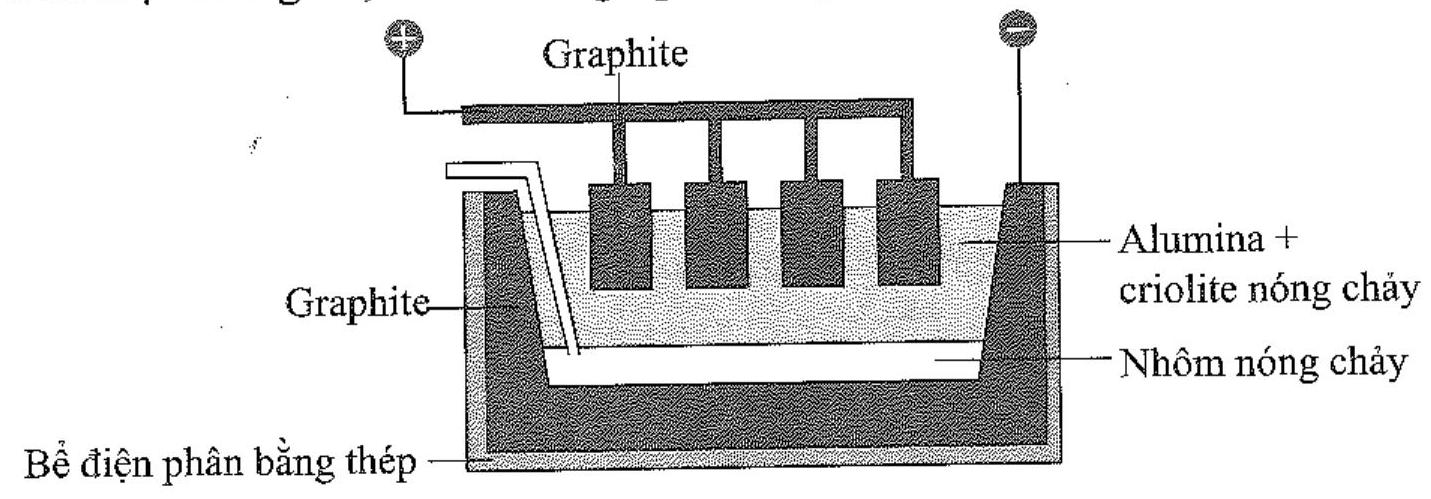
\includegraphics[width=\textwidth]{2025_10_23_80c1361fcdcd395cad8eg-48}
\captionsetup{labelformat=empty}
\caption{Hìnih 15.1. Mô hình quy trình Hall - Héroult}
\end{center}
\end{figure}

Mỗi phát biểu sau đây là đúng hay sai?\\
(a) Nhôm kim loại được tách ra tại cathode.\\
(b) Cryolite được thêm vào bể điện phân giúp tiết kiệm năng lượng, giảm chi phí sản xuất.\\
(c) Bên cạnh nhôm, oxygen tinh khiết cũng có thể thu được trực tiếp từ quy trình này.\\
(d) Vì anode và cathode đều làm bằng graphite, nên nếu đổi chiều dòng điện (anode trở thành cathode và ngược lại) thì quy trình điện phân vẫn diễn ra bình thường.\\[0pt]
[1] \href{https://www.vinmec.com/vi/y-hoc-co-truyen/duoc-lieu/cay-chu-sa-co-tac-dung-gi/}{https://www.vinmec.com/vi/y-hoc-co-truyen/duoc-lieu/cay-chu-sa-co-tac-dung-gi/}, truy cập ngày 20/02/2024.

\section*{BAI \\
 16. HỢP KIM - SỰ̆ ĂN MÒN KIM LOAI}
16.1. Nối các hợp kim ở cột A với kỉm loại cơ bản - kim loại là thành phần chính tương ứng ở cột B .

\section*{Cột $\mathbf{A}$}
\begin{enumerate}
  \item Gang
  \item Thép
  \item Dural
  \item Bronze
  \item Inox
  \item Thiếc hàn
\end{enumerate}

\section*{Côt B}
a) Al\\
b) Cu\\
c) Fe\\
d) Sn\\
16.2. Những phát biểu nào sau đây là đúng?\\
(a) Hợp kim được sử dụng trong đời sống và sản xuất phổ biến hơn so với kim loại.\\
(b) Kim loại $\mathbb{A}$ có nhiệt độ nóng chảy cao hơn kim loại $\mathbb{B}$, nhiệt độ nóng chảy của hợp kim $\mathbf{A}-\mathbf{B}$ luôn cao hơn nhiệt độ nóng chảy của $\mathbf{B}$.\\
(c) Tính chất hoá học của hợp kim thường tương tự tính chất của các kim loại thành phần.\\
(d) Hợp kim có thể cứng hơn rất nhiều các kim loại tạo nên nó.\\
(e) Hợp kim thường khó bị oxi hoá hơn các đơn kim loại thành phần.\\
16.3. "Thép 304" là một loại thép không gỉ được dùng phổ biến trong đời sống. Các kim loại chủ yếu tạo nên loại thép này bao gồm:\\
A. $\mathrm{Fe}, \mathrm{C}, \mathrm{Cr}$.\\
B. $\mathrm{Fe}, \mathrm{Cu}, \mathrm{Cr}$.\\
C. $\mathrm{Fe}, \mathrm{Cr}, \mathrm{Ni}$.\\
D, $\mathrm{Fe}, \mathrm{C}, \mathrm{Cr}, \mathrm{Ni}$.\\
16.4. Để lợp nhà, các tấm tôn (thép mỏng mạ kẽm) được gắn với nhau bởi các đinh thép. Theo thòi gian, các tấm tôn bị ăn mòn. Những nhận định nào sau đây là đúng?\\
(1) Vị trí đóng đinh thép dễ xảy ra ăn mòn hơn các vị trí khác.\\
(2) Tấm tôn bị ăn mòn từ trong ra ngoài do thép bị ăn mòn trước kẽm.\\
(3) Sắt trong tấm tôn không bị ăn mòn theo thời gian.\\
(4) Lớp tráng kẽm bị ăn mòn trước.\\
A. (1), (2).\\
B. (1), (4).\\
C. (2), (3).\\
D. (1), (3), (4).\\
16.5. Trang sức bằng bạc có thể bị ăn mòn bởi oxygen không khí khi có mặt hydrogen sulfide, tạo thành silver sulfide có màu đen. Viết phương trình hoá học của phản ứng xảy ra. Trong trường hợp này, bạc bị ăn mòn theo dạng ăn mòn hoá học hay ăn mòn điện hoá? Cho biết vai trò của oxygen trong quá trình này.\\
16.6. Những phát biểu nào sau đây là đúng khi nói về sự ăm mòn của gang, thép trong không khí ẩm?\\
(a) Dạng ăn mòn hoá học là chủ yếu, do sắt dễ dàng phản ứng với oxygen trong không khí.\\
(b) Carbon bị khử tai cathode.\\
(c) Oxygen đóng vai trò là chất oxi hoá.\\
(d) Tại anode, Fe bị oxi hoá thành $\mathrm{Fe}^{2+}$.\\
(e) Carbon đóng vai trò là cực âm (anode), sắt là cực dương (cathode) khi sự ăn mòn xảy ra.\\
16.7. Dural là một loại hợp kim quan trọng của nhôm, có đặc điểm là nhẹ, cứng, bền cơ học phù hợp với các ứng dụng nào sau đây?\\
(1) Chế tạo cánh máy bay.\\
(2) Áo giáp, khiên bảo vệ.\\
(3) Làm ống dẫn dầu, mỏ neo.\\
A. (1), (2).\\
B. (1).\\
C. (1), (2), (3).\\
D. (1), (3).\\
$16.8^{*}$. Để chống ăn mòn cho vỏ tàu biển làm bằng thép, bên cạnh việc phủ mặt ngoài của vỏ tàu bằng sơn, nhà sản xuất còn gắn nhiều khối kẽm lên mặt ngoài vỏ tàu (phần chìm trong nước). Phương pháp này còn được gọi là "anode hi sinh". Tìm hiểu và giải thích vì sao phương pháp này lại có tên gọi như vậy. Bên cạnh vỏ tàu biển, phương pháp này còn có thể áp dụng cho những trường hợp nào khác? Tìm hiểu và nêu một vài ví dụ.\\
16.9. Những trường hợp nào sau đây có xảy ra ăn mòn điện hoá? Giải thích.\\
a) Cho một mẩu sodium vào dung dịch copper(II) sulfate.\\
b) Nhúng một thanh kẽm vào dung dịch silver nitrate.\\
c) Nhúng một thanh sắt vào dung dịch iron(III) chloride.\\
d) Cho nước vào hỗn hợp bột magnesium, sắt và muối ăn.\\
e) Trộn bột Zn vào bột $\mathrm{CuSO}_{4}$.\\
16.10. Thực hiện thí nghiệm sau:

Bước 1: Cho dung dịch $\mathrm{NaCl} 5 \%$ vào ống thuỷ tinh hình chữ U như hình bên.

Bước 2: Nhúng một thanh đồng và một thanh kẽm đã làm sạch vào hai đầu của ống chữ U.\\
、Bước 3: Nối hai thanh kim loại bằng dây dẫn.\\
a) Sau bước 2, kim loại nào bị ăn mòn?\\
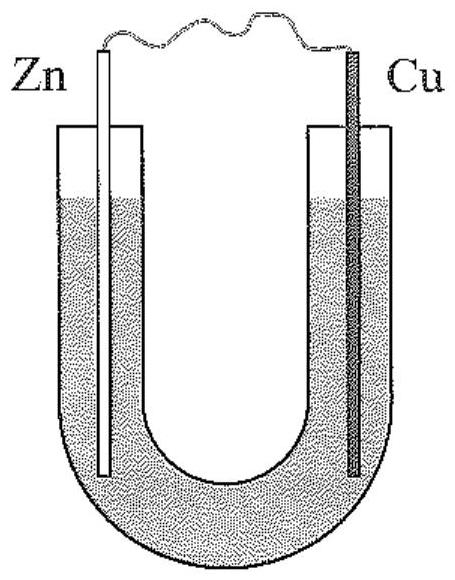
\includegraphics[max width=\textwidth, center]{2025_10_23_80c1361fcdcd395cad8eg-51}\\
A. Đồng.\\
B. Kẽm.\\
C. Cả hai đều bị ăn mòn.\\
D. Không kim loại nào bị ăn mòn.\\
b) Sau bước 3 , những phát biểu nào sau đây đúng?\\
(1) Hai kim loại kẽm và đồng đều bị ăn mòn.\\
(2) Kẽm bị oxi hoá và đóng vai trò là anode.\\
(3) $\mathrm{Cu}^{2+}$ bị khử thành Cu bám vào thanh đồng, làm khối lượng thanh đồng tăng dần.\\
(4) Không kim loại nào bị ăn mòn, nếu thay dung dịch NaCl thành dung dịch HCl thì ăn mòn mới diễn ra.\\
(5) Kẽm bị ăn mòn, đồng không bị ăn mòn.\\
c) Khoảng vài phút sau bước 3 , nhỏ vài giọt phenolphthalein vào dung dịch gần thanh đồng và quan sát thấy dung dịch dần chuyển sang màu hồng là do\\
A. dòng điện từ ăn mòn điện hoá đã điện phân NaCl thành dung dịch NaOH .\\
B. sự khử oxygen hoà tan trong dung dịch tạo môi trường base.\\
C. sự thuỷ phân muối NaCl làm tăng pH của dung dịch.\\
D. do phản ứng giữa Cu và dung dịch NaCl tạo hợp chất có tính base.

\section*{CHỦ DỀ 7 'NGUYÊN TỐ NHÓM IA VÀ NHÓM IIA}
\section*{Bal 17 NGUYÊN TỐ NHÓM IA}
17.1. Trong tự nhiên, các nguyên tố nhóm IA chỉ tồn tại ở dạng hợp chất là do\\
A. các nguyên tố nhóm IA chỉ có thể được tìm thấy trong nước ngầm, nước biển.\\
B. các nguyên tố ñhóm IA đều là những kim loại hoạt động hoá học mạnh nên không tồn tại dạng đơn chất.\\
C. các nguyên tố nhóm IA thường kết hợp với nhau để tạo thành các hợp kim bền.\\
D. các nguyên tố nhóm IA có độ âm điện lớn nên dễ dàng kết hợp với các nguyên tố khác.\\
17.2. Những phát biểu nào sau đây là đúng về các nguyên tố nhóm IA?\\
(a) Có cấu hình electron lớp ngoài cùng là $\mathrm{ns}^{1}(\mathrm{n}>1)$.\\
(b) Có số oxi hoá là +1 hoặc +2 trong các hợp chất.\\
(c) Có tính khử mạnh.\\
(d) Có bán kính nguyên tử nhỏ.\\
(e) Còn được gọi là các kim loại kiềm.\\
17.3. Những đặc điểm chung nào của các kim loại kiềm ( M ) sau đây có thể guíp dự đoán chúng đều có tính khử mạnh?\\
(a) Kim loại M trong cặp oxi hoá - khử $\mathrm{M}^{+} / \mathrm{M}$ có thế điện cực chuẩn ( $\mathrm{E}_{\mathrm{M}^{+} / \mathrm{M}}^{\circ}$ ) rất âm.\\
(b) Mềm và dễ nóng chảy.\\
(c) Có nhiều electron hoá trị nên dễ dàng nhường electron.\\
(d) Lực hút của hạt nhân đối với electron hoá trị trong kim loại kiềm yếu hơn so với lực hút tương ứng ở các kim loại nhóm khác.\\
(e) Có cấu trúc tinh thể rỗng.\\
17.4. Những lĩnh vực nào sau đây ứng dụng nhiều kim loại nhóm IA và các hợp chất của chúng?\\
(a) xây dựng, công nghiệp ô tô, luyện kim.\\
(b) sản xuất pháo hoa.\\
(c) sản xuất phân bón.\\
(d) chế biến thực phẩm.\\
(e) pin, đồng hồ nguyên tử.\\
17.5. Giá trị biến thiên enthalpy tạo thành chuẩn $\left(\mathrm{kJ} \mathrm{mol}^{-1}\right)$ của $\mathrm{NaHCO}_{3}(s), \mathrm{Na}_{2} \mathrm{CO}_{3}(s)$, $\mathrm{CO}_{2}(g)$ và $\mathrm{H}_{2} \mathrm{O}(g)$ lần lượt là $-950,81 ;-1130,70 ;-393,51$ và $-241,80$.\\
a) Tính giá trị biến thiên enthalpy chuẩn của phản ứng sau:

$$
2 \mathrm{NaHCO}_{3}(s) \rightarrow \mathrm{Na}_{2} \mathrm{CO}_{3}(s)+\mathrm{H}_{2} \mathrm{O}(g)+\mathrm{CO}_{2}(g)
$$

b) Phản ứng trến có thuận lợi về mặt năng lượng không?\\
c) Theo em, vì sao baking soda không bị phân huỷ theo phản ứng ở ý a) khi được bảo quản ở nơi thoáng mát?\\
17.6. Các kim loại kiềm có khối lượng riêng nhỏ và độ cứng thấp hơn nhiều so với các kim loại khác. Nguyên nhân là do:\\
(1) Tinh thể có kiểu mạng lập phương tâm khối.\\
(2) Khối lượng nguyên tử nhỏ hon các kim loại khác.\\
(3) Có lực liên kết kim loại yếu.\\
A. (1), (2) và (3).\\
B. (2) và (3).\\
C. (1) và (3).\\
D. (1) và (2).\\
17.7. Dãy nào sau đây sắp xếp đúng các kim loại theo chiều tăng dần nhiệt độ nóng chảy?\\
A. $\mathrm{Hg}, \mathrm{Cs}, \mathrm{K}, \mathrm{Na}, \mathrm{Fe}, \mathrm{W}$.\\
B. $\mathrm{Hg}, \mathrm{Na}, \mathrm{K}, \mathrm{Cs}, \mathrm{W}, \mathrm{Fe}$.\\
C. $\mathrm{Cs}, \mathrm{K}, \mathrm{Na}, \mathrm{Hg}, \mathrm{Fe}, \mathrm{W}$.\\
D. Hg, Cs, Na, K, Fe, W.\\
17.8. Cho một mẩu sodium nhỏ vào cốc nước có chứa vài giọt phenolphthalein. Mỗi phát biểu sau đây là đúng hay sai?\\
(a) Sodium bị hoà tan nhanh chóng là do hiện tượng ăn mòn điện hoá.\\
(b) Cốc nước chuyển từ không màu sang màu hồng.\\
(c) Khí thoát ra trong thí nghiệm là một khí dễ cháy.\\
(d) Nếu thay mẩu sodium bằng mẩu lithium cùng kích thước thì phản ứng diễn ra chậm hơn.\\
17.9. Dừng panh lấy các mẩu kim loại ( $\mathrm{Li}, \mathrm{Na}$ hoặc K ) có kích cỡ xấp xỉ nhau đã thấm khô dầu và cho vào chậu thuỷ tinh đã chứa khoảng $1 / 3$ thể tích nước. Thêm $2-3$ giọt dung dịch phenolphthalein vào chậu sau khi kim loại tan hết. Mỗi phát biểu sau đây đúng hay sai?\\
(a) Các dung dịch thu được sau phản ứng đều có màu hồng.\\
(b) Trong nước, potassium tan nhanh hon so với sodium, sodium tan nhanh hon so với lithium.\\
(c) Các cặp oxi hoá - khử $\mathrm{M}^{+} / \mathrm{M}(\mathrm{M}: \mathrm{Li}, \mathrm{Na}, \mathrm{K})$ đều có giá trị thế điện cực chuẩn lón hơn giá trị thế điện cực chuẩn của cặp oxi hoá - khử $2 \mathrm{H}_{2} \mathrm{O} / \mathrm{H}_{2}+2 \mathrm{OH}^{-}$.\\
(d) Kết quả thí nghiệm cho kết luận tính khử của các kim loại tăng dần theo dãy $\mathrm{K}, \mathrm{Na}, \mathrm{Li}$.\\
17.10. Trong các phản ứng sau đây, phản ứng nào diễn ra mãnh liệt nhất?\\
A. Lithium và bromine.\\
B. Potassium và chlorine.\\
C. Lithium và chlorine.\\
D. Sodium và bromine.\\
17.11*. Nhúng que plàtinum sạch vào dung dịch chất X , sau đó đưa lên ngọn lửa đèn khí, đèn khí cháy với ngọn lửa màu vàng. Mặt khác, thêm vài giọt dung dịch chất $X$ vào dung dịch silver nitrate thấy xuất hiện kết tủa vàng. $X$ có thể là chất nào sau đây?\\
(1) Potassium iodide.\\
(2) Sodium iodide.\\
(3) Sodium phosphate.\\
(4) Potassium phosphate.\\
A. (1) hoặc (4).\\
B. (2) hoặc (3).\\
C. (2).\\
D. (3) hoặc (4).\\
17.12. Viết phương trình hoá học của phản ứng xảy ra khi thực hiện phản ứng giữa sodium lần lượt với lượng dư chlorine, oxygen và lưu huỳnh. Giả sử sodium bị oxi hoá hết trong mỗi phản ứng.\\
Cho một lượng nước thích hợp vào mỗi sản phẩm thu được ở trên để thu được các dung dịch có nồng độ khoảng $0,1 \mathrm{M}$. Dự đoán pH của mỗi dung dịch thu được và giải thích.\\
17.13. Công đoạn chính của công nghiệp chlorine - kiềm là điện phân dung dịch sodium chloride bão hoà trong bể điện phân có màng ngăn xốp. Phương trình hoá học của quá trình điện phân là: $2 \mathrm{NaCl}+2 \mathrm{H}_{2} \mathrm{O} \rightarrow 2 \mathrm{NaOH}+\mathrm{H}_{2}+\mathrm{Cl}_{2}$.\\
Mỗi phát biểu sau đây là đúng hay sai?\\
(a) Anion $\mathrm{Cl}^{-}$bị khử thành khí chlorine tại anode.\\
(b) Tại cathode, thu được đồng thời dung dịch bão hoà và tinh thể sodium hydroxide.\\
(c) Nếu không có màng ngăn xốp, nước Javel được hình thành trong bể diện phân.\\
(d) Hydrogen cũng là một sản phẩm có giá trị của công nghiệp chlorine - kiềm.\\
17.14. Trong thực tế, trong quá trình điện phân dung dịch sodium chloride bão hoà, sau một thời gian, dung dịch NaCl tại anode được gọi là "nước muối nghèo" và được đưa ra khỏi bể điện phân; đồng thời dung dịch NaCl bão hoà mới được bổ sung vào để tiếp tục quá trình điện phân (như Hình 17.1). Hãy giải thích việc làm này, viết phương trình hoá học (nếu có). Biết rằng, dung dich tại bể anode có $\mathrm{pH}=3 ; \mathrm{E}_{\mathrm{Cl}_{2} / 2 \mathrm{Cl}}^{\circ}=1,36 \mathrm{~V} ; \mathrm{E}_{\mathrm{O}_{2}, 4 \mathrm{H}^{\prime} / 2 \mathrm{H}_{2} \mathrm{O}}^{\circ}=1,23 \mathrm{~V}$.

Nước muối bão hoà có nồng độ $300 \mathrm{~g} \mathrm{~L}^{-1}$, trong khi đó "nước muối nghèo" có nồng độ $220 \mathrm{~g} \mathrm{~L}^{-1}$. Với mỗi lít nước muối bão hoà ban đầu thì thu được bao nhiêu gam sodium hydroxide, nếu hiệu suất của quá trình là $80 \%$ ?

\begin{figure}[h]
\begin{center}
  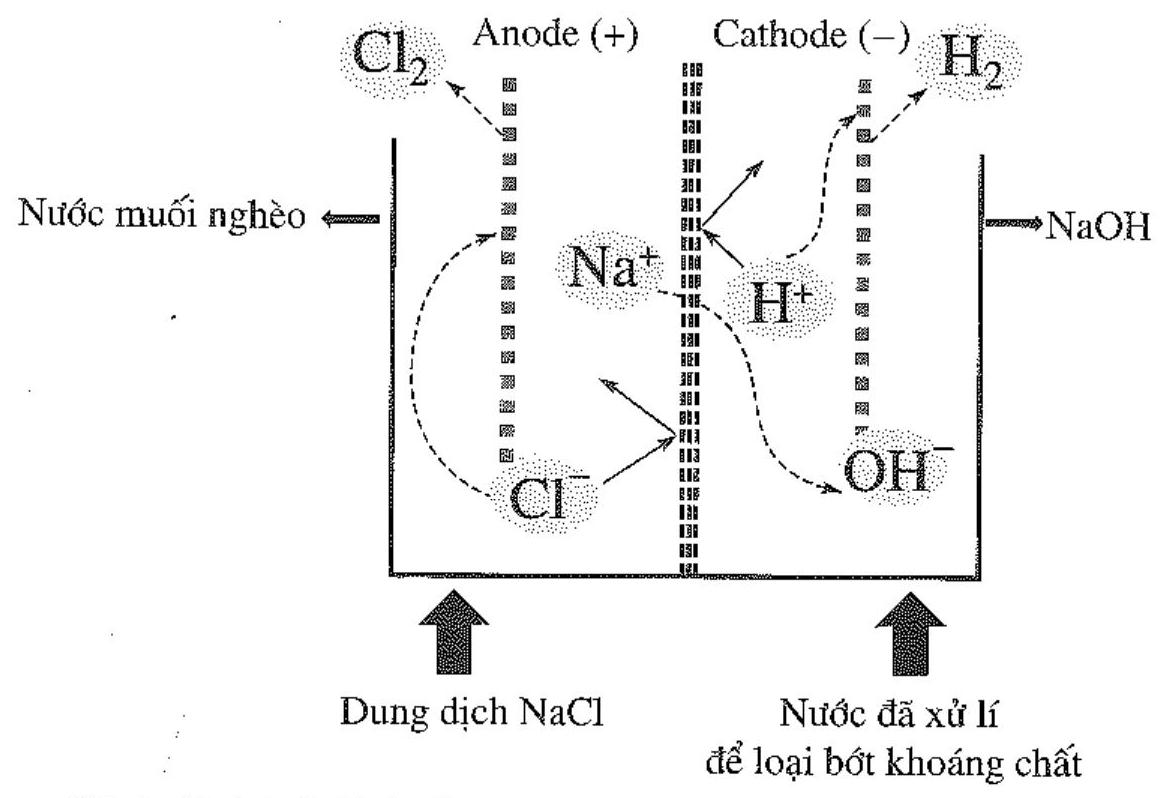
\includegraphics[width=\textwidth]{2025_10_23_80c1361fcdcd395cad8eg-55}
\captionsetup{labelformat=empty}
\caption{Hình 17.1. Mô hình điện phân dung dịch sodium chloride bão hoà}
\end{center}
\end{figure}

17.15. Những phát biểu nào sau đây là đúng về hợp chất sodium hydrogencarbonate?\\
(1) Còn gọi là sodium bicarbonate hay baking soda.\\
(2) Được dùng để điều trị chứng dư acid trong dạ dày, làm mềm thực phẩm.\\
(3) Là chất dạng bột màu trắng, dễ bị oxi hoá bởi oxygen trong không khí.\\
A. (1) và (2).\\
B. (1), (2) và (3).\\
C. (1) và (3).\\
D. (2).\\
17.16. Những phát biểu nào sau đây là đúng?\\
(a) Soda là chất bột màu trắng, tan trong nước tạo môi trường trung tính.\\
(b) Soda có thể được dùng để làm mềm nước cứng.\\
(c) Soda bền với nhiệt hơn so với baking soda.\\
(d) Chất béo có thể bị thuỷ phân trong dung dịch soda tạo thành xà phòng.\\
(e) Có thể dùng baking soda thay cho soda trong việc tẩy rửa lớp dầu, mõ bám vào bồn rửa.\\
17.17. Soda được sản xuất theo phương pháp Solvay theo các phương trình hoá học sau:


\begin{align*}
& \mathrm{NaCl}(a q)+\mathrm{CO}_{2}(g)+\mathrm{H}_{2} \mathrm{O}(l)+\mathrm{NH}_{3}(a q) \rightarrow \mathrm{NaHCO}_{3}(s)+\mathrm{NH}_{4} \mathrm{Cl}(a q)  \tag{1}\\
& 2 \mathrm{NaHCO}_{3}(s) \xrightarrow{\mathrm{t}^{\mathrm{o}}} \mathrm{Na}_{2} \mathrm{CO}_{3}(s)+\mathrm{CO}_{2}(g)+\mathrm{H}_{2} \mathrm{O}(g)  \tag{2}\\
& 2 \mathrm{NH}_{4} \mathrm{Cl}(a q)+\mathrm{CaO}(s) \rightarrow 2 \mathrm{NH}_{3}(g)+\mathrm{CaCl}_{2}(a q)+\mathrm{H}_{2} \mathrm{O}(l) \tag{3}
\end{align*}


Những phát biểu nào sau đây là không đúng?\\
(a) Phản ứng (1) cho thấy $\mathrm{H}_{2} \mathrm{CO}_{3}\left(\mathrm{CO}_{2}+\mathrm{H}_{2} \mathrm{O}\right)$ có tính acid mạnh hơn dung dịch HCl .\\
(b) Muối sodium hydrogencarbonate ít tan trong nước và kém bền khi bị nung nóng.\\
(c) Phản ứng (3) nhằm thu hồi và tái sử dụng $\mathrm{NH}_{3}$.\\
(d) Trong phản ứng (2) khối lượng chất rắn giảm $45 \%$ sau khi nung (giả sử hiệu suất nung là $100 \%$ ).\\
17.18. Nhiệt tạo thành của một số chất được cho trong bảng sau:

\begin{center}
\begin{tabular}{|c|c|c|c|c|c|}
\hline
$\mathrm{Chát}^{2}$ & $\mathrm{Na}_{2} \mathrm{CO}_{3}(s)$ & $\mathrm{NaHCO}_{3}(s)$ & $\mathrm{Na}_{2} \mathrm{O}(s)$ & $\mathrm{CO}_{2}(g)$ & $\mathrm{H}_{2} \mathrm{O}(l)$ \\
\hline
$\Delta \mathrm{H}_{298}^{\mathrm{o}}\left(\mathrm{kl} \mathrm{mol}^{-1}\right)$ & $-1130,70$ & $-950,81$ & $-414,20$ & $-393,51$ & $-285,83$ \\
\hline
\end{tabular}
\end{center}

Mỗi phát biểu sau đây là đúng hay sai?\\
(a) Quá trình hình thành muối $\mathrm{NaHCO}_{3}$ từ các đơn chất thuận lợi về năng lượng hơn so với quá trình hình thành muối $\mathrm{Na}_{2} \mathrm{CO}_{3}$ từ các đơn chất.\\
(b) Giá trị biến thiên enthalpy chuẩn của phản ứng

$$
2 \mathrm{NaHCO}_{3}(s) \rightarrow \mathrm{Na}_{2} \mathrm{CO}_{3}(s)+\mathrm{H}_{2} \mathrm{O}(l)+\mathrm{CO}_{2}(g) \text { là }-91,28 \mathrm{~kJ}
$$

(c) Phản ứng $\mathrm{Na}_{2} \mathrm{CO}_{3}(s) \rightarrow \mathrm{Na}_{2} \mathrm{O}(s)+\mathrm{CO}_{2}(g)$ không diễn ra ở điều kiện thường, phù hợp với giá trị biến thiên enthalpy chuẩn của phản ứng khá dương.\\
(d) $\mathrm{Na}_{2} \mathrm{CO}_{3}$ bền với nhiệt hơn $\mathrm{NaHCO}_{3}$.

\section*{1821 18 NGUYÊN TỐ NHÓM IIA}
18.1. Nguyên tố nhóm IIA được tìm thấy trong tự nhiên dưới dạng nào?\\
(1) Các cation $\mathrm{M}^{2+}$ trong nước ao hồ, nước ngầm.\\
(2) Các khoáng vật ít tan như carbonate, sulfate, silicate.\\
(3) Các hợp chất it tan trong răng, xương động vật.\\
A. (1) và (2).\\
B. (1) và (3).\\
C. (1), (2) và (3).\\
D. (2) và (3).\\
18.2. Những phát biểu nào sau đây là đúng?\\
(a) Số oxi hoá của các nguyên tố kim loại nhóm IIA trong hợp chất là +1 hoặc +2 .\\
(b) Beryllium là kim loại nhẹ nhất trong các kim loại nhóm IIA.\\
(c) Magnesium là kim loại có nhiệt độ nóng chảy thấp nhất trong nhóm IIA.\\
(d) Các kim loại nhóm IIA đều có cấu trúc mạng tinh thể lập phương tâm khối.\\
(e) Các kim loại nhóm IIA đều dẫn điện.\\
18.3. Dãy các kim loại nào sau đây tác dụng nhanh với nước ở điều kiện thường?\\
A. $\mathrm{Be}, \mathrm{Na}, \mathrm{Ba}$.\\
B. $\mathrm{Mg}, \mathrm{Ca}, \mathrm{Ba}$.\\
C. $\mathrm{Li}, \mathrm{Ca}, \mathrm{Ba}$.\\
D. $\mathrm{Sr}, \mathrm{Sn}, \mathrm{Ba}$.\\
18.4. Barium phản ứng với nước dễ dàng hơn so với magnesium ở điều kiện thường là do các nguyên nhân nào sau đây?\\
(1) Barium có tính khử mạnh hơn magnesium.\\
(2) Độ tan của barium hydroxide trong nước cao hơn nhiều so với magnesium hydroxide.\\
(3) Bọt khí hydrogen sinh ra bám trên bề mặt magnesium nhiều hơn, cản trở phản ứng tiếp diễn.\\
A. (1).\\
B. (1), (2) và (3).\\
C. (1) và (3).\\
D. (1) và (2).\\
18.5. Thực hiện phản ứng giữa các dung dịch sau:\\
a) Potassium carbonate và calcium hydroxide.\\
b) Sodium phosphate và barium chloride.\\
c) Magnesium hydrogencarbonate và sulfuric acid.\\
d) Sodium hydrogencarbonate và barium hydroxide.\\
e) Barium hydroxide và nitric acid.

Những phản ứng nào thu được kết tủa? Viết phương trình hoá học của các phản ứng xảy ra.\\
18.6. Những phát biểu nào sau đây về ứng dụng của một số hợp chất của calcium là đúng?\\
(a) Vôi tôi và vôi sống đều có thể dùng để khử chua đất trong nông nghiệp.\\
(b) Đá vôi và thạch cao đều được dùng trong sản xuất vật liệu xây dựng.\\
(c) Khoáng vật apatite được khai thác để sản xuất phân đạm.\\
(d) Vôi tôi có thể được dùng để làm mềm nước cứng.\\
(e) Thạch cao còn được dùng trong y tế như bó bột cố định xương.\\
18.7. Tìm hiểu và cho biết vai trò của calcium đối với cơ thể người và các vấn đề sức khoẻ có thể mắc phải khi thiếu hụt calcium. Liệt kê một số thực phẩm phù hợp để cung cấp calcium cho cơ thể.\\
18.8. Một học sinh thực hiện các thí nghiệm để nhận biết hai dung dịch chất X và chất Y , thu được một số kết quả như sau:

\begin{itemize}
  \item Dung dịch chất $\mathbb{X}$ và chất $\mathbb{Y}$ đều làm dung dịch phenolphthalein chuyển sang màu hồng.
  \item Trộn $X$ và $Y$ thu được kết tủa màu trắng.
  \item Chất $\mathbf{X}$ cháy với ngọn lửa màu lục trên đèn khí, trong khi chất $\mathbf{Y}$ cháy với ngọn lửa màu tím.\\
Mỗi kết luận sau đây của học sinh đó về chất X và chất Y là đúng hay sai? Biết mỗi chất $\mathbf{X}, \mathbf{Y}$ đều chỉ chứa một loại cation và một loại anion.\\
(a) Chất X có chứa cation $\mathrm{Ba}^{2+}$, chất Y chứa cation $\mathrm{K}^{+}$.\\
(b) Chất X không thể là barium chloride.\\
(c) Chất Y phải là potassium carbonate.\\
(d) Kết tủa màu trắng phải là hợp chất của barium.\\
18.9. Nhiệt độ phân huỷ thành oxide của các muối carbonate của kim loại nhóm IIA giảm dần theo dãy\\
A. $\mathrm{MgCO}_{3}, \mathrm{CaCO}_{3}, \mathrm{SrCO}_{3}, \mathrm{BaCO}_{3}$.\\
B. $\mathrm{BaCO}_{3}, \mathrm{SrCO}_{3}, \mathrm{CaCO}_{3}, \mathrm{MgCO}_{3}$.\\
C. $\mathrm{BaCO}_{3}, \mathrm{CaCO}_{3}, \mathrm{SrCO}_{3}, \mathrm{MgCO}_{3}$.\\
D. $\mathrm{MgCO}_{3}, \mathrm{BaCO}_{3}, \mathrm{SrCO}_{3}, \mathrm{CaCO}_{3}$.\\
18.10. Xét các phản ứng phân huỷ sau:
\end{itemize}


\begin{equation*}
\mathrm{CaCO}_{3}(s) \rightleftharpoons \mathrm{CaO}(s)+\mathrm{CO}_{2}(g) \tag{1}
\end{equation*}



\begin{equation*}
\mathrm{BaCO}_{3}(s) \rightleftharpoons \mathrm{BaO}(s)+\mathrm{CO}_{2}(g) \tag{2}
\end{equation*}


Biến thiên enthalpy chuần ( $\Delta_{\mathrm{r}} \mathrm{H}_{298}^{\circ}$ ) của phản ứng thuận ở mỗi cân bằng (1) và (2) khi phân huỷ 1 mol mỗi chất lần lượt có giá trị là $108,7 \mathrm{~kJ}$ và $271,5 \mathrm{~kJ}$. Những phát biểu nào sau đây là đúng?\\
(a) Nhiệt lượng toả ra khi phân huỷ $1 \mathrm{~mol} \mathrm{BaCO}_{3}$ lớn hơn nhiệt lượng toả ra khi phân huỷ $1 \mathrm{~mol} \mathrm{CaCO}_{3}$.\\
(b) $\mathrm{BaCO}_{3}$ bị phân hử ở nhiệt độ cao hơn $\mathrm{CaCO}_{3}$.\\
(c) Khi tăng nhiệt độ, cả hai phản ứng đều dịch chuyển theo chiều thuận.\\
(d) $\mathrm{CO}_{2}$ cần được lấy ra khỏi lò nung để tăng hiệu suất của phản ứng.\\
18.11. Beryllium carbonate $\left(\mathrm{BeCO}_{3}\right)$ khan là chất bột màu trắng, dễ phân huỷ ngay trong điều kiện thường, tạo thành beryllium oxide. Do đó, $\mathrm{BeCO}_{3}$ thường được bảo quản trong khí quyển tạo bởi chất X . Giống như các muối carbonate của các kim loại nhóm IIA khác, $\mathrm{BeCO}_{3}$ it tan trong nước; tuy nhiên, điểm khác biệt là chất này dễ bị thuỷ phân tạo thành các dạng tồn tại khác của beryllium như $\mathrm{Be}(\mathrm{OH})_{3}^{-}, \mathrm{Be}(\mathrm{OH})_{4}^{2-}$. Điều này chủ yếu là do cation $\mathrm{Be}^{2+}$ có bán kính nhỏ hơn nhiều so với các cation kim loại cùng nhóm IIA. Việc thường xuyên hít phải $\mathrm{BeCO}_{3}$ hay BeO đều có thể dẫn tới ung thư phổi. Nếu đi vào cơ thể, các cation $\mathrm{Be}^{2+}$ có thể vô hiệu hoá chức năng của các enzyme, đặc biệt là các enzyme chưa phức chất có nguyên tử trung tâm được hình thành từ cation $\mathrm{Mg}^{2+[\mathrm{I}]}$.\\
Mỗi phát biểu sau đây là đúng hay sai?\\
(a) Phần trăm khối lượng của beryllium trong beryllium carbonate tinh khiết khan là $6,25 \%$.\\
(b) Khí X là carbon dioxide.\\
(c) Mật độ điện tích của ion bằng điện tích của ion chia cho thể tích của ion đó. Ion được coi có dạng cầu nện thể tích của ion tỉ lệ với luỹ thừa 3 của bán kính ion.\\
Cation $\mathrm{Be}^{2+}$ dễ bị thuỷ phân hơn so với cation $\mathrm{Ca}^{2+}$ là do mật độ điện tích trên cation $\mathrm{Be}^{2+}$ nhỏ hơn so với cation $\mathrm{Ca}^{2+}$.\\
(d) Cation $\mathrm{Be}^{2+}$ có khả năng thay thế nguyên tử trung tâm magnesium của phức chất trong một số enzyme, tạo phức chất bền hơn.\\
18.12. a) Barium nitrate là hợp chất cộng hoá trị hay hợp chất ion, là chất dễ tan hay ít tan trong nước?\\
b) Hoàn thành các phương trình hoá học sau:\\
(1) $\mathrm{Ba}\left(\mathrm{NO}_{3}\right)_{2}(s) \xrightarrow{\mathfrak{t}^{\circ}}$ ?\\
(2) $\mathrm{Ba}\left(\mathrm{NO}_{3}\right)_{2}(a q)+\mathrm{Na}_{2} \mathrm{SO}_{4}(a q) \rightarrow$ ?\\
c) Độ tan trong nước của $\mathrm{Ba}\left(\mathrm{NO}_{3}\right)_{2}$ ở $10^{\circ} \mathrm{C}$ và $20^{\circ} \mathrm{C}$ lần lượt là $6,67 \mathrm{~g} / 100 \mathrm{~g}$ nước và $9,02 \mathrm{~g} / 100 \mathrm{~g}$ nước. Khi đưa $109,02 \mathrm{~g}$ dung dịch $\mathrm{Ba}\left(\mathrm{NO}_{3}\right)_{2}$ bão hoà ở $20^{\circ} \mathrm{C}$ về $10^{\circ} \mathrm{C}$ thì thu được bao nhiêu gam tinh thể $\mathrm{Ba}\left(\mathrm{NO}_{3}\right)_{2} \cdot 6 \mathrm{H}_{2} \mathrm{O}$ kết tinh?\\
d) Cho các hoá chất cơ bản sau: dung dịch NaOH , dung dịch HCl , dung dịch $\mathrm{H}_{2} \mathrm{SO}_{4}$, dung dịch NaCl . Hoá chất nào trong các hoá chất trên có thể được dùng để nhận biết được ion $\mathrm{Ba}^{2+}$ trong dung dịch barium nitrate? Viết phương trình hoá học minh hoạ.\\
18.13. Gói làm nóng thức ăn (FRH: Flameless Ration Heater) được phát minh nhằm hâm nóng các bữa ăn tiện lợi cho người lính trên chiến trường. Một số gói lẩu tự sôi cũng sử dụng công nghệ này. FRH có thành phần chính gồm bột kim loại Mg trộn với một lượng nhỏ bột Fe và NaCl . Khi sử dụng, chỉ cần cho khoảng 30 mL nước vào hỗn hợp FRH , hỗn hợp này phản ứng mãnh liệt theo phương trình $\mathrm{Mg}+2 \mathrm{H}_{2} \mathrm{O} \rightarrow \mathrm{Mg}(\mathrm{OH})_{2}+\mathrm{H}_{2}$ và toả rát nhiều nhiệt, đủ để làm nóng thức ăn nhanh chóng.\\
a) Một gói FRH chứa khoảng 8 gam hỗn hợp ( $\mathrm{Mg} 90 \%, \mathrm{Fe} 4 \%$ và $\mathrm{NaCl} 6 \%$ về khối lượng) có thể toả ra tối đa bao nhiêu nhiệt để làm nóng? Biết rằng enthalpy tạo thành chuẩn $\left(\triangle_{\mathrm{f}} \mathrm{H}_{298}^{\mathrm{o}}\right)$ của $\mathrm{Mg}(\mathrm{OH})_{2}(s)$ và $\mathrm{H}_{2} \mathrm{O}(l)$ lần lượt là $-928,4 \mathrm{~kJ} \mathrm{~mol}^{-1}$ và $-285,8 \mathrm{~kJ} \mathrm{~mol}^{-1}$. Gói FRH trên có đủ làm nóng 300 g súp từ $30^{\circ} \mathrm{C}$ lên $100^{\circ} \mathrm{C}$ hay không? Biết nhiệt dung của súp khoảng $4,2 \mathrm{~J} \mathrm{~g}^{-1}{ }^{\circ} \mathrm{C}^{-1}$, giả sử gói súp chỉ nhận được $50 \%$ lượng nhiệt tối đa toả ra, phần nhiệt còn lại làm nóng các vật dụng khác và thất thoát vào môi trường.\\
b) Magnesium phản ứng chậm với nước ở nhiệt độ thường, giải thích vì sao magnesium trong gói FRH lại có thể phản ứng nhanh chóng với nước.\\
c) Ví sao người ta chỉ dùng khoảng 30 mL nước mà không dùng lượng nước nhiều hơn ${ }^{[1]}$ ?

\footnotetext{[1] \href{https://patents.google.com/patent/US4017414}{https://patents.google.com/patent/US4017414}, truy cập ngày 20/02/2024.
}\section*{Bil 19 NUOÓC CÚNG VÀ LÀM MỀM NUỚC CỨNG}
19.1. Những loại nước nào sau đây không phải là nước cửng?\\
(a) Nước có chưa nhiều ion $\mathrm{Ca}^{2+}$.\\
(b) Nước có chứa nhiều ion $\mathrm{Ca}^{2+}, \mathrm{Mg}^{2+}, \mathrm{HCO}_{3}^{-}$.\\
(c) Nước có chưa ít ion $\mathrm{Ca}^{2+}, \mathrm{Mg}^{2+}$.\\
(d) Nước có chứa ít ion $\mathrm{Ca}^{2+}$ nhưng chứa nhiều ion $\mathrm{Mg}^{2+}$ và $\mathrm{Cl}^{-}$.\\
(e) Nước chỉ chứa nhiều ion $\mathrm{Na}^{+}, \mathrm{Cu}^{2+}, \mathrm{HCO}_{3}^{-}$.\\
19.2. Những phát biểu nào sau đây về nước có tính cứng tạm thời là đúng?\\
(a) Chứa nhiều ion $\mathrm{HCO}_{3}^{-}$.\\
(b) Chỉ chứa 2 loại cation $\mathrm{Mg}^{2+}$ và $\mathrm{Ca}^{2+}$.\\
(c) Có thể loại bỏ tính cứng tạm thời của nước bằng cách dùng lượng vừa đủ $\mathrm{Ca}(\mathrm{OH})_{2}$ hoặc $\mathrm{Na}_{2} \mathrm{CO}_{3}$.\\
(d) Không gây nhiều tác hại như nước có tính cứng vĩnh cửu hay nước cứng toàn phần.\\
(e) Có thể được làm mềm bằng phương pháp trao đồi ion.\\
19.3. Đặc điểm nào sau đây là điểm chung của nước có tính cứng vĩnh cửu và nước có tính cứng toàn phần?\\
A. Đều có thể làm mềm bằng $\mathrm{Na}_{3} \mathrm{PO}_{4}$.\\
B. Đều không chứa anion $\mathrm{HCO}_{3}^{-}$.\\
C. Đều bị mất một phần tính cứng khi đun sôi nước.\\
D. Thành phần anion giống nhau.\\
19.4. Những phát biểu nào sau đây là đúng?\\
(a) Nước có chứa nhiều ion $\mathrm{HCO}_{3}^{-}$được gọi là nước có tính cứng tạm thòi.\\
(b) Có thể làm mềm nước có tính cứng tạm thời bằng cách đun sôi nước.\\
(c) Có thể loại bỏ một phần tính cứng của nước có tính cứng vĩnh cửu bằng cách dùng một lượng vừa đủ $\mathrm{Ca}(\mathrm{OH})_{2}$.\\
(d) Không thể dùng cách đun sôi để loại bỏ hoàn toàn tính cứng của nước có chứa nhiều các ion sau: $\mathrm{Mg}^{2+}, \mathrm{Ca}^{2+}, \mathrm{Cl}^{-}, \mathrm{HCO}_{3}^{-}, \mathrm{SO}_{4}^{2-}$.\\
(e) Nước cứng có thể là nguyên nhân gây nổ nồi hơi.\\
19.5. Dùng dung dịch $\mathrm{Ca}(\mathrm{OH})_{2}$ với lượng vừa đủ có thể làm mềm nước có tính cứng tạm thời, giải thích và viết phương trình hoá học của phản ứng (nếu có).\\
19.6. Hoàn thành bảng sau bằng cách điền dấu X vào ô ứng với thông tin đúng.

\begin{center}
\begin{tabular}{|l|l|l|l|}
\hline
Mọt só dạc điêm & Nước có tính cứng tam thơi & Nước có tinh cưng toan phần & Nước có tinh cưng vĩnh cưu \\
\hline
(1) Chứa nhiều ion $\mathrm{Mg}^{2+}, \mathrm{Ca}^{2+}$ & ? & ? & ? \\
\hline
(2) Gây đóng cặn nồi hơi, làm quần áo mau mục nát, giảm hương vị thực phẩm & ? & ? & ? \\
\hline
(3) Loại bỏ được một phần hoặc hoàn toàn tính cứng khi đun sôi nước & ? & ? & ? \\
\hline
(4) Loại bỏ được hoàn toàn tính cúng khi dùng lượng vừa đủ $\mathrm{Ca}(\mathrm{OH})_{2}$ & ? & ? & ? \\
\hline
(5) Có thể làm mềm bằng $\mathrm{Na}_{2} \mathrm{CO}_{3}$, $\mathrm{Na}_{3} \mathrm{PO}_{4}$ & ? & ? & ? \\
\hline
(6) Có thể làm mềm bằng phương pháp trao đổi ion & ? & ? & ? \\
\hline
\end{tabular}
\end{center}

19.7. Một mẫu nước cứng có nồng độ các ion $\mathrm{Na}^{+}, \mathrm{Ca}^{2+}, \mathrm{Mg}^{2+}, \mathrm{Cl}^{-}, \mathrm{SO}_{4}^{2-}$ và $\mathrm{HCO}_{3}^{-}$tương ứng là: $1,2 \mathrm{mM} ; 3,0 \mathrm{mM} ; 1,0 \mathrm{mM} ; 0,6 \mathrm{mM} ; 0,1 \mathrm{mM}$ và x mM $\left(1 \mathrm{mM}=1 \mathrm{mmol} \mathrm{L}^{-1}\right)$, ngoài ra không chứa ion nào khác.\\
a) Có thể làm mất tính cứng của loại nước này khi đun sôi hay không?\\
b) Tính tổng khối lượng chất tan còn lại sau khi đun sôi kĩ 2 lít mẫu nước cứng này. Giả sử các muối $\mathrm{MgCO}_{3}, \mathrm{CaCO}_{3}$ hầu như không tan trong nước.

\section*{CHỦDỀ 8 SƠ LƯỢC VỀ KIM LOAI CHUYỂN TIẾP DÃY THỨ NHẤT VÀ PHỨC CHẤT}
\section*{Pal}
\section*{20 SO LƯỢC VỀ KIM LOAI CHUYỂN TIỂP DÃY THỨ NHẤT}
20.1. Trong bảng tuần hoàn các nguyên tố hoá học, nguyên tố chuyển tiếp dãy thứ nhất được xếp ở\\
A. chu kì 3.\\
B. chu kì 4.\\
C. chu kì 5.\\
D. chu kì 3 và chu kì 4 .\\
20.2. Các electron hoá trị của nguyên tử nguyên tố kim loại chuyển tiếp dãy thứ nhất phân bố ở\\
A. phân lớp 3 d và phân lớp 4 s .\\
B. phân lớp 3d.\\
C. lớp 4s.\\
D. phân lớp 3p và phân lớp 3d.\\
20.3. Cho phát biểu "Nguyên tố kim loại chuyển tiếp dãy thứ nhất tạo nhiều hợp chất mà trong đó chúng có các số oxi hoá dương khác nhau, đó là do nguyên tố này có ...(1)... và nguyên tử của chúng có ...(2)..." Cụm từ cần điền vào (1) và (2) lần lượt là:\\
A. độ âm điện bé, nhiều electron hoá trị.\\
B. độ âm điện lớn, nhiều electron hoá trị.\\
C. điện tích hạt nhân lớn, bán kính bé.\\
D. bán kính bé, điện tích hạt nhân lớn.\\
20.4. Theo IUPAC, nguyên tố chuyển tiếp là những nguyên tố có phân lớp d chưa được xếp (hoặc điền) đầy electron ở trạng thái nguyên tử hoặc ở trạng thái ion. Mỗi phát biểu dưới đây đúng hay sai?\\
(a) Calcium không phải là nguyên tố chuyển tiếp do không có phân lớp d trong cấu hình electron của nguyên tư.\\
(b) Nguyên tố có $Z=30$ là nguyên tố chuyển tiếp.\\
(c) Nguyên tố có $Z=29$ không phải là nguyên tố chuyển tiếp.\\
(d) Nguyên tố chuyển tiếp có tính kim loại nên còn được gọi là nguyên tố kim loại chuyển tiếp.\\
20.5. Từ kết quả phân tích phổ phát xa nguyên tử của chromium ( $\mathrm{Z}=24$ ) dẫn đến nhận định rằng nguyên tử này phải có 6 electron độc thân.\\
Mỗi phát biểu dưới đây đúng hay sai?\\
(a) Nếu nguyên tự chromium có 6 electron độc thân thì nguyên tử này chứa 6 ô orbital nguyên tử mà trong mỗi ô này chỉ có 1 electron.\\
(b) Theo các quy ước về viết cấu hình electron thì cấu hình electron của nguyên tử chromium là $[\mathrm{Ar}] 3 \mathrm{~d}^{3} 4 \mathrm{~s}^{1} 4 \mathrm{p}^{1}$.\\
(c) Cấu hình electron của nguyên tử là $[\mathrm{Ar}] 3 \mathrm{~d}^{5} 4 \mathrm{~s}^{1}$ sẽ phù hợp với nhận định từ phổ phát xạ của nguyên tử chromium.\\
(d) Cấu hình electron của nguyên tử phải luôn phù hợp với các quy ước về viết cấu hình electron.\\
20.6. Những đặc điểm nào sau đây là của nguyên tố kim loại chuyển tiếp dãy thứ nhất?\\
(a) Có các electron hoá trị phân bố cả trên phân lớp 3d và phân lớp 4s.\\
(b) Từ ${ }_{21} \mathrm{Sc}$ đến ${ }_{29} \mathrm{Cu}$, số electron trong phân lớp d có xu hướng tăng dần (trừ trường hợp ngoại lệ).\\
(c) Thể hiện nhiều số oxi hoá dương hoặc âm trong các hợp chất.\\
(d) Tạo nên pihiều cation và anion có điện tích khác nhau.\\
20.7. Số electron hoá trị của nguyên tử sắt $(\mathrm{Z}=26)$ là bao nhiêu?\\
20.8. Số electron độc thân của nguyên tử cobalt $(\mathrm{Z}=27)$ là bao nhiêu?\\
20.9. Hợp chất $\mathrm{Fe}_{3} \mathrm{O}_{4}$ được gọi là oxide sắt từ do có từ tính mạnh. Chất này còn có tên gọi là iron(II, III) oxide do đây là hỗn hợp của FeO và $\mathrm{Fe}_{2} \mathrm{O}_{3}$ theo tỉ lệ mol 1:1.\\
a) Theo quá trình: $\mathrm{Fe}_{3} \mathrm{O}_{4}(s)+\mathrm{HCl}(a q) \rightarrow \mathrm{FeCl}_{2}(a q)+\mathrm{FeCl}_{3}(a q)+\mathrm{H}_{2} \mathrm{O}(l)$ thì số mol HCl trong dung dịch hydrochloric acid cần để hoà tan vừa đủ $1 \mathrm{~mol} \mathrm{Fe}_{3} \mathrm{O}_{4}$ là bao nhiêu?\\
b) Trong tự nhiên, $\mathrm{Fe}_{3} \mathrm{O}_{4}$ là thành phần chính của khoáng vật magnetite, được dửng tạo sắt nóng chảy trong quá trình sản xuất thép.\\
(b1) Viết phương trình hoá học của phản ứng xảy ra khi khử $\mathrm{Fe}_{3} \mathrm{O}_{4}$ thành sắt bới carbon monoxide ở nhiệt độ cao.\\
(b2) Trong phản ứng trên, số electron mà 1 phân tử $\mathrm{Fe}_{3} \mathrm{O}_{4}$ cần nhận để tạo thành sắt là bao nhiêu?\\
20.10. Giải thích vì sao:\\
a) số oxi hoá lớn nhất của nguyên tố manganese là +7 ?\\
b) hợp chất $\mathrm{KMnO}_{4}$ có tính oxi hoá mạnh?\\
c) số oxi hoá lớn nhất của nguyên tố chromium là +6 ?\\
d) hợp chất $\mathrm{K}_{2} \mathrm{CrO}_{4}$ có tính oxi hoá mạnh?\\
e) sắt là nguyên tố chuyển tiếp?\\
g) trong tự nhiên, cation $\mathrm{Fe}^{3+}$ thường phổ biến hơn cation $\mathrm{Fe}^{2+}$ ?\\
h) cation $\mathrm{Fe}^{2+}$ có cả tính oxi hoá và tính khử?\\
20.11. Tìm hiểu, cho biết những phát biểu nào sau đây là đúng.\\
(a) Ở dạng đơn chất, sắt là kim loại nặng, có độ hoạt động hoá học mạnh.\\
(b) Sắt ít được sử dụng ở dạng nguyên chất. Sắt chủ yếu được sử dụng ở dạng hợp kim (thép thường, inox,...).\\
(c) Đinh đóng gỗ được làm bằng thép nhưng vẫn bị gỉ sét do ăn mòn điện hoá.\\
(d) Số oxi hoá của sắt trong các hợp chất $\mathrm{FeO}, \mathrm{Fe}_{2} \mathrm{O}_{3}$ và $\mathrm{FeO}(\mathrm{OH}) \cdot \mathrm{H}_{2} \mathrm{O}$ lần lượt là $+2,+3$ và +3 .\\
(e) Thành phần chính của gỉ sét, của váng nâu đỏ ở vùng nước nhiễm phèn là $\mathrm{FeO}(\mathrm{OH}) \cdot \mathrm{H}_{2} \mathrm{O}$ hay $\mathrm{Fe}(\mathrm{OH})_{3}$.\\
20.12. Giải thích vì sao:\\
a) có thể phân biệt các dung dịch $\mathrm{CuSO}_{4}, \mathrm{CoSO}_{4}, \mathrm{FeSO}_{4}, \mathrm{NiSO}_{4}$ và $\mathrm{CrSO}_{4}$ thông qua quan sát?\\
b) có thể phân biệt được hai muối $\mathrm{K}_{2} \mathrm{CrO}_{4}$ và $\mathrm{K}_{2} \mathrm{Cr}_{2} \mathrm{O}_{7}$ thông qua quan sát?\\
c) có thể nhận biết cation $\mathrm{Cu}^{2+}$ trong dung dịch bằng dung dịch base?\\
d) có thể nhận biết cation $\mathrm{Fe}^{3+}$ trong dung dịch bằng dung dịch base?\\
20.13. Hoà tan $0,422 \mathrm{~g}$ mẫu khoáng vật của sắt trong dung dịch sulfuric acid dư, sao cho tất cả lượng sắt có trong quặng đều chuyển thành $\mathrm{Fe}^{2+}$, thu được dung dịch A . Chuẩn độ $\mathrm{Fe}^{2+}$ trong dung dịch A bằng chất chuẩn là dung dịch thuốc tím $\mathrm{KMnO}_{4} 0,040 \mathrm{M}$. Khi đã sử dụng $23,50 \mathrm{~mL}$ thì phản ứng vừa qua điểm tương đương.\\
Mỗi phát biểu dưới đây là đúng hay sai?\\
(a) Nếu chỉ có $\mathrm{Fe}^{2+}$ trong dung dịch A tác dụng được với thuốc tím thì việc chuẩn độ dung dịch A sẽ giúp xác định được lượng nguyên tố sắt trong mẫu khoáng vật. Từ đó tính được \% (theo khối lượng) của nguyên tố sắt có trong mẫu khoáng vật là $60,26 \%$.\\
(b) Trong quá trình chuẩn độ trên, cần nhỏ từ từ dung dịch thuốc tím từ burette vào bình tam giác chưa dung dịch A .\\
(c) Cần thêm chất chỉ thị phù hợp vào bình tam giác chứa dung dịch A để xác định được thời điểm kết thúc quá trình chuẩn độ.\\
(d) Cần lặp lại thí nghiệm chuẩn độ 2 lần để bảo đảm tính chính xác của kết quả.\\
20.14. Cho các thông tin sau:

\begin{center}
\begin{tabular}{|l|c|}
\hline
\multicolumn{1}{|c|}{Cạp oxi hoá- khư} & Thế diến cực chuấn (V) \\
\hline
$\mathrm{Fe}^{3+} / \mathrm{Fe}^{2+}$ & $-0,77$ \\
\hline
$\mathrm{Cr}_{2} \mathrm{O}_{7}^{2-}+14 \mathrm{H}^{+} / 2 \mathrm{Cr}^{3+}+7 \mathrm{H}_{2} \mathrm{O}$ & 1,33 \\
\hline
$\mathrm{MnO}_{4}^{-}+8 \mathrm{H}^{+} / \mathrm{Mn}^{2+}+4 \mathrm{H}_{2} \mathrm{O}$ & 1,53 \\
\hline
\end{tabular}
\end{center}

Biết $\mathrm{Cr}_{2} \mathrm{O}_{7}^{2-}(a q)$ có màu cam và $\mathrm{Cr}^{3+}(a q)$ có màu xanh lá cây.\\
Mỗi phát biểu dưới đây đúng hay sai?\\
(a) Trong môi trường acid, anion $\mathrm{Cr}_{2} \mathrm{O}_{7}^{2-}$ (từ sự phân li của muối potassium dichromate, $\mathrm{K}_{2} \mathrm{Cr}_{2} \mathrm{O}_{7}$ ) có tính oxi hoá mạnh hơn anion $\mathrm{MnO}_{4}^{-}$(từ sự phân li của muối $\mathrm{KMnO}_{4}$ ).\\
(b) Chuẩn độ được $\mathrm{Fe}^{2+}$ trong dung dịch gồm $\mathrm{Fe}^{2+}, \mathrm{SO}_{4}^{2-}$ và $\mathrm{H}^{+}$bằng dung dịch chứa chất chuẩn là $\mathrm{KMnO}_{4}$.\\
(c) Không chuẩn độ được $\mathrm{Fe}^{2+}$ trong dung dịch gồm $\mathrm{Fe}^{2+}, \mathrm{SO}_{4}^{2-}$ và $\mathrm{H}^{+}$bằng dung dịch chứa chất chuẩn là $\mathrm{K}_{2} \mathrm{Cr}_{2} \mathrm{O}_{7}$.\\
(d) Có diễn ra phản ứng oxi hoá - khử theo phương trình hoá học sau:

$$
6 \mathrm{Fe}^{3+}(a q)+2 \mathrm{Cr}^{3+}(a q)+7 \mathrm{H}_{2} \mathrm{O}(l) \rightarrow 6 \mathrm{Fe}^{2+}(a q)+\mathrm{Cr}_{2} \mathrm{O}_{7}^{2-}(a q)+14 \mathrm{H}^{+}(a q)
$$

20.15. Dựa vào Bảng 20.4 (sách Hoá học 12 , bộ sách Cánh Diều), hãy chỉ ra những phát biểu đúng.\\
(a) Các kim loại chuyển tiếp thường cứng và khó nóng chảy.\\
(b) Các kim loại chuyển tiếp được xếp vào nhóm kim loại nhẹ.\\
(c) So với calcium (là kim loại s), các kim loại chuyển tiếp dãy thứ nhất có khối lượng riêng, độ cứng và nhiệt độ nóng chảy thấp hơn.\\
(d) Nhờ có độ cứng cao, đồng thời bền trước tác động của các tác nhân ăn mòn nên chromium được dùng làm lớp bảo vệ chống ăn mòn cho các dụng cụ, máy móc, thiết bị, đồ gia dụng,...\\
(e) Do có độ cứng vừa phải và dẫn điện tốt nên đồng được sử dụng làm dây dẫn trong các thiết bị và mạng lưới điện gia dụng.\\
21.1. Cho phát biểu sau: "Phức chất đơn giản thường có một ...(1)... liên kết với các phối tử bao quanh. Liên kết giữa nguyên tử trung tâm và phối tử trong phức chất là liên kết ... (2)....". Cụm từ cần điền vào (1) và (2) lần lượt là\\
A. cation kim loại, ion.\\
B. nguyên tử kim loại, cho - nhận.\\
C. nguyên tữ trung tâm, cho - nhận.\\
D. phối tử, ion.\\
21.2. Theo thuyết Liên kết hoá trị, để trở thành phối tử trong phức chất thì phân tử hoặc anion cần có\\
A. các orbital trống.\\
B. cặp electron hoá trị riêng.\\
C. ît nhất 4 orbital trống.\\
D. ít nhất hai cặp electron hoá trị riêng.\\
21.3. Cho các chất có công thức: $\mathrm{CuCl}_{2}, \mathrm{NH}_{3},\left[\mathrm{CuCl}_{4}\right]^{2-}$. Phát biểu nào sau đây là không đúng?\\
A. Do không có liên kết cộng hoá trị theo kiểu cho - nhận trong phân tử nên $\mathrm{CuCl}_{2}$ không phải là phức chất.\\
B. Do có nguyên tử trung tâm là nguyên tố kim loại, đồng thời các phối tử xung quanh liên kết với nguyên tử trung tâm bằng liên kết cho - nhận nên $\left[\mathrm{CuCl}_{4}\right]^{2-}$ là phức chất.\\
C. Dừ có các nguyên tử H xung quanh N , nhưng $\mathrm{NH}_{3}$ không phải là phức chất.\\
D. Do nguyên tố đồng có hoá trị II nên quanh nguyên tử Cu trong $\mathrm{CuCl}_{2}$ và trong $\left[\mathrm{CuCl}_{4}\right]^{2-}$ đều có 2 liên kết.\\
21.4. Phát biểu nào sau đây không đúng về phức chất?\\
A. Phức chất đơn giản thường có một nguyên tử trung tâm liên kết với các phối tử bao quanh.\\
B. Phức chất có thể mang điện tích hoặc không mang điện tích.\\
C. Liên kết giữa nguyên tử trung tâm và phối tử trong phức chất là liên kết ion.\\
D. $\mathrm{K}_{2}\left[\mathrm{PtCl}_{4}\right]$ hoặc anion $\left[\mathrm{PtCl}_{4}\right]^{2-}$ đều được xếp vào loại phức chất.\\
21.5. Những phát biểu nào sau đây là không đúng về nguyên tử trung tâm trong phức chất?\\
(a) Nguyên tử trung tâm trong phức chất là cation kim loại hoặc nguyên tử kim loại đã nhận cặp electron hoá trị riêng của phân tử hoặc anion.\\
(b) Cation tạo nguyên tử trung tâm trong phức chất $\left[\mathrm{Co}\left(\mathrm{OH}_{2}\right)_{6}\right]^{3+}$ là $\mathrm{Co}^{3+}$.\\
(c) Nguyên tử trung tâm trong phức chất là các nguyên tố kỉm loại chuyển tiếp.\\
(d) Nguyên tử trung tâm trong phức chất $\left[\mathrm{Ni}(\mathrm{CO})_{4}\right]$ được hình thành từ quá trình cation $\mathrm{Ni}^{2+}$ sử dụng các orbital trống để nhận các cặp electron hoá trị của các phân tử CO .\\
21.6. Theo thuyết Liên kết hoá trị, những phát biểu nào sau đây là không đúng?\\
(a) Phối tử là các phân tử hoặc anion đã cho một hoặc một số cặp electron hoá trị riêng.\\
(b) Các phần tử gồm $\mathrm{NH}_{3}, \mathrm{~N}_{2}, \mathrm{H}_{2}, \mathrm{OH}^{-}, \mathrm{Cl}^{-}$đều có thể trở thành phối tử trong phức chất.\\
(c) Cóphốitừ là anion và phốitửlà phân tử trong phức chất[ $\left.\mathrm{Cu}\left(\mathrm{NH}_{3}\right)_{4}\left(\mathrm{OH}_{2}\right)_{2}\right]^{2+}$.\\
(d) Khi tham gia quá trình tạo phức chất, phân tử ethylenediamine $\mathrm{H}_{2} \mathrm{~N}-\mathrm{CH}_{2}-\mathrm{CH}_{2}-\mathrm{NH}_{2}$ sử dụng hai cặp electron hoá trị riêng để tạo 2 liên kết cho - nhận.\\
21.7. Những phát biểu nào sau đây về dạng hình học của phức chất là đúng?\\
(a) Phức chất mà xung quanh nguyên tử trung tâm có 4 liên kết $\sigma$ thường có dạng hình học là tứ diện hoặc vuông phẳng và được gọi là phức chất tứ diện hoặc phức chất vuông phẳng.\\
(b) Phức chất mà xung quanh nguyên tử trung tâm có 6 liên kết $\sigma$ có dạng hình học là bát diện và được gọi là phức chất bát diện.\\
(c) Hai liên kết $\mathrm{Pt}-\mathrm{Cl}$ kế cận nhau trong anion $\left[\mathrm{PtCl}_{4}\right]^{2-}$ tạo thành một góc liên kết. Thực nghiệm xác nhận trong anion $\left[\mathrm{PtCl}_{4}\right]^{2-}$ có bốn góc liên kết đều có giá trị xấp xi $90^{\circ}$. Vi vậy, $\left[\mathrm{PtCl}_{4}\right]^{2-}$ là phức chất vuông phẳng.\\
(d) Dạng hình học của phức chất được xác nhận bằng thực nghiệm.\\
21.8. Những phát biểu nào sau đây về phức chất bát diện $\left[\mathrm{Cu}\left(\mathrm{OH}_{2}\right)_{6}\right]^{2+}$ là đúng?\\
(a) Nguyên tử trung tâm được hình thành từ quá trình cation $\mathrm{Cu}^{2+}$ sử dụng 6 orbital trống để nhận các cặp electron hoá trị riêng của các phân tử $\mathrm{H}_{2} \mathrm{O}$.\\
(b) Số oxi hoá của nguyên tử trung tâm là +2 .\\
(c) Số liên kết cho - nhận giữa phối tử và nguyên tử trung tâm cũng là hoá trị phổ biến của đồng.\\
(d) Mỗi phân tử nước chỉ sử dụng 1 trong 2 cặp electron hoá trị riêng của nó để tạo liên kết cho - nhận với cation $\mathrm{Cu}^{2+}$.\\
21.9. Những phát biểu nào sau đây về phức chất $\mathrm{Na}_{3}\left[\mathrm{Co}\left(\mathrm{NO}_{2}\right)_{6}\right]$ là đúng?\\
(a) Có liên kết cho - nhận và liên kết ion trong phân tử.\\
(b) Có anion $\left[\mathrm{Co}\left(\mathrm{NO}_{2}\right)_{6}\right]^{3-}$ cũng là một phức chất.\\
(c) Có nguyên tử trung tâm là natri (sodium) và cobalt.\\
(d) Nguyên tữ trung tâm có số oxi hoá là +2 .\\
21.10. Cho hai phức chất $\mathbb{A}$ và $\mathbb{B}$ có công thức lần lượt sau:\\
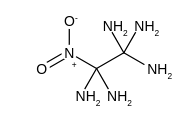
\includegraphics{smile-e0aef3923a84f36338d2f465f2695420597f5779}

Mỗi phát biểu sau đây đúng hay sai?\\
(a) Nguyên tử trung tâm của hai phức chất đều là nguyên tố kim loại chuyển tiếp.\\
(b) Trong phức chất B có 4 phối tử.\\
(c) Hai phức chất $\mathbf{A}$ và $\mathbf{B}$ có dạng hình học khác nhau.\\
(d) Trong A và trong B đều có hai loại phối tử.\\
21.11. Nối những đặc điểm ở cột B với phức chất tương ứng ở cột A .

Biết rằng khi ion $\mathrm{Cr}^{3+}$ hoặc nguyên tử Cr tạo phức chất thì trở thành nguyên tử trung tâm chromium có 6 liên kết cho - nhận với các phối tử xung quanh.

\section*{Cột ${ }^{4}$}
\begin{enumerate}
  \item $\left[\mathrm{Cr}(\mathrm{en})_{3}\right]^{3+}$
  \item $\left[\mathrm{Cr}\left(\mathrm{NH}_{3}\right)_{6}\right]^{3+}$
  \item $\left[\mathrm{Cr}(\mathrm{CO})_{6}\right]$
\end{enumerate}

B\\
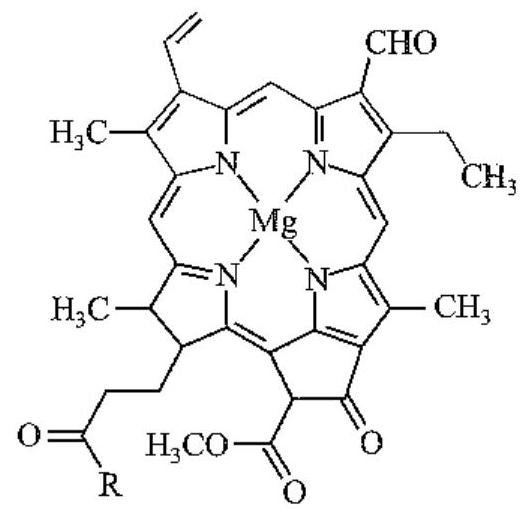
\includegraphics[max width=\textwidth, center]{2025_10_23_80c1361fcdcd395cad8eg-69}

\section*{Cột B}
a) Một phối tử chỉ tạo một liên kết cho - nhận với nguyên tử trung tâm\\
b) Một phối tử tạo hai liên kết cho - nhận với nguyên tử trung tâm\\
c) Là phức chất trung hoà\\
d) Là phức chất ion\\
e) Nguyên tử trung tâm được hình thành từ quá trình cation kim loại nhận các cặp electron hoá trị\\
g) Nguyên tử trung tâm được hình thành từ quá trình nguyên tử kim loại nhận các cặp electron hoá trị\\
21.12. Mỗi phân tử ethylenediamine ( $\mathrm{H}_{2} \mathrm{~N}-\mathrm{CH}_{2}-\mathrm{CH}_{2}-\mathrm{NH}_{2}$ ):\\
a) có bao nhiêu cặp electron hoá trị riêng có thể được dùng để tạo phức chất với cation kim loại?\\
b) có luôn dùng tất cả các cặp electron hoá trị riêng để tạo liên kết với cation kim loại không?\\
21.13. Xét phân tử $\mathrm{H}_{2} \mathrm{O}$, phân tử hydrazine $\mathrm{H}_{2} \mathrm{~N}-\mathrm{CH}_{2}-\mathrm{NH}_{2}$ và anion $\mathrm{F}^{-}$. Cho biết:\\
a) Mỗi phân tử hoặc anion trên có bao nhiêu cặp electron hoá trị riêng?\\
b) Vì sao 1 phân tử $\mathrm{H}_{2} \mathrm{O}$ hoặc 1 phân tử $\mathrm{H}_{2} \mathrm{~N}-\mathrm{CH}_{2}-\mathrm{NH}_{2}$ hay 1 anion F chỉ sử dụng được một cặp electron hoá trị riêng để tạo liên kết với cation kim loại trong quá trỉnh hình thành phức chất?\\
c) Khi tạo phức chất, cation $\mathrm{Co}^{3+}$ nhận được 6 cặp electron hoá trị riêng từ các phối tử. Hãy cho biết giá trị x và n trong công thức $\left[\mathrm{CoF}_{\mathrm{x}}\right]^{\mathrm{n}-}$ là bao nhiêu. Giải thích.\\
21.14. Các phức chất được tạo thành từ sự tương tác giữa cation $\mathrm{Co}^{3+}$ với đồng thời cả anion $\mathrm{C}_{2} \mathrm{O}_{4}^{2-}$ (kí hiệu là ox) và phân tử $\mathrm{H}_{2} \mathrm{O}$, có dạng $\left[\mathrm{Co}\left(\mathrm{OH}_{2}\right)_{\mathrm{x}}(\mathrm{ox})_{\mathrm{y}}\right]^{\mathrm{p}+}$ và $\left[\mathrm{Co}\left(\mathrm{OH}_{2}\right)_{\mathrm{a}}(\mathrm{ox})_{\mathrm{b}}\right]^{\mathrm{a}-}$.\\
Biết rằng trong các phức chất này:

\begin{itemize}
  \item Cation $\mathrm{Co}^{3+}$ tạo được 6 liên kết sigma kiểu cho - nhận với các phối tử.
  \item Mỗi anion $\mathrm{C}_{2} \mathrm{O}_{4}^{2-}$ sử dụng 2 cặp electron hoá trị riêng để tạo liên kết cho - nhận với cation kim loại.
  \item Mỗi phân tử $\mathrm{H}_{2} \mathrm{O}$ sử dụng 1 cặp electron hoá trị riêng để tạo liên kết cho - nhận với cation kim loại.\\
Hãy đề xuất công thức của các phức chất phù hợp với những dữ liệu trên.\\
21.15. Khi hoà tan hỗn hợp gồm muối cobalt(III) chloride và sodium chloride vào nước thì một số quá trình cơ bản sau sẽ diễn ra:
\end{itemize}

\[
\begin{array}{ll}
\mathrm{NaCl} & \rightarrow \mathrm{Na}^{+}+? \\
\mathrm{CoCl}_{3} & \rightarrow \mathrm{Co}^{3+}+3 \mathrm{Cl}^{-} \\
\mathrm{Co}^{3+}+? & \rightarrow\left[\mathrm{Co}\left(\mathrm{OH}_{2}\right)_{6}\right]^{3+} \\
\mathrm{Na}^{+}+? & \rightarrow \mathrm{Na}^{+}\left(\mathrm{H}_{2} \mathrm{O}\right)_{\mathrm{x}} \\
\mathrm{Cl}^{-}+? & \rightarrow \mathrm{Cl}^{-}\left(\mathrm{H}_{2} \mathrm{O}\right)_{\mathrm{y}} \tag{5}
\end{array}
\]

a) Điền thông tin phù hợp vào các dấu ? ở các quá trình trên.\\
b) Với các quá trình trên, chỉ ra quá trình hydrate hoá, quá trình tạo phức chất và quá trình phân li.\\
c) Nêu các đặc điểm về liên kết hoặc tương tác trong mỗi sản phẩm ghi ở (3), (4) và (5).\\
d) Theo em, vì sao ở (4) và (5) không hình thành phức chất?\\
21.16. a) Vì sao AgCl không phải là phúc chất trong khi cation $\left[\mathrm{H}_{3} \mathrm{~N}-\mathrm{Ag}-\mathrm{NH}_{3}\right]^{+}$ là phức chất?\\
b) Vì sao sodium chloride $(\mathrm{NaCl})$ không phải là một phức chất?

\section*{Bin SƠ LƯỢC VỀ SỰ HÌNH THÀNH PHỨC CHẤT CỦA ION KIM LOAI CHUYỂN TIẾP TRONG DUNG DICH}
22.1. Cho phát biểu sau: "Khi tan trong nước, muối của các kim loại chuyển tiếp $\ldots$ (1) $\ldots$ thành các ion. Sau đó, cation kim loại chuyển tiếp $\left(\mathrm{M}^{\mathrm{n}+}\right)$ thường nhận các cặp electron hoá trị riêng từ các phân tử $\mathrm{H}_{2} \mathrm{O}$ để hình thành các liên kết cho - nhận, tạo ra phức chất aqua có dạng tổng quát là ...(2)....\\
Cựm từ cần điền vào (1) và (2) lần lượt là:\\
A. điện li, $\left[\mathrm{M}\left(\mathrm{OH}_{2}\right)_{n}\right]^{+}$.\\
B. điện $\mathrm{li},\left[\mathrm{M}\left(\mathrm{OH}_{2}\right)_{\mathrm{m}}\right]^{\mathrm{n}+}$.\\
C. phân li, $\left[\mathrm{M}\left(\mathrm{OH}_{2}\right)_{\mathrm{m}}\right]^{\mathrm{n}+}$.\\
D. phân li, $\left[\mathrm{M}\left(\mathrm{OH}_{2}\right)_{\mathrm{n}}\right]^{+}$.\\
22.2. Khi cho dung dịch ammonia dư vào dung dịch chứa phức chất $\left[\mathrm{Ni}\left(\mathrm{OH}_{2}\right)_{6}\right]^{2+}$ và anion $\mathrm{Cl}^{-}$thì có phản ứng sau:

$$
\left[\mathrm{Ni}\left(\mathrm{OH}_{2}\right)_{6}\right]^{2+}(a q)+6 \mathrm{NH}_{3}(a q) \rightarrow\left[\mathrm{Ni}\left(\mathrm{NH}_{3}\right)_{6}\right]^{2+}(a q)+6 \mathrm{H}_{2} \mathrm{O}(l)\left(^{*}\right)
$$

Phát biểu nào dưới đây là không đúng?\\
A. Trong điều kiện của phản ứng (\textit{), phức chất [ $\left.\mathrm{Ni}\left(\mathrm{NH}_{3}\right)_{6}\right]^{2+}(a q)$ kém bền hơn phức chất $\left[\mathrm{Ni}\left(\mathrm{OH}_{2}\right)_{6}\right]^{2+}(a q)$.\\
B. Phản ứng (}) là phản ứng thế phối tử.\\
C. Dung dịch sau phản ứng có $\mathrm{pH}>7$.\\
D. Trong phản ứng không có sự thay đổi số oxi hoá của các nguyên tố.\\
22.3. Nước có lượng đáng kể các cation $\mathrm{Al}^{3+}$ và $\mathrm{Fe}^{3+}$ được gọi là nước nhiễm phèn. Trong nước nhiễm phèn, mỗi cation này bị thuỷ phân tạo thành phức chất gồm 1 nguyên tử trung tâm, 3 phối tử $\mathrm{OH}^{-}$và 3 phối tử $\mathrm{H}_{2} \mathrm{O}$.\\
a) Viết phương trình hoá học của các phản ứng diễn ra.\\
b) Vì sao nước phèn có pH thấp?\\
c) Vì sao trong nước phèn xuất hiện các chất lơ lửng không tan?\\
22.4. Muối cobalt(II) chloride có màu hồng. Hoà tan muối này vào nước thu được dung dịch màu xanh (dung dịch A ) do ion $\mathrm{Co}^{2+}$ tạo thành phức chất aqua có dạng hình học bát diện. Phức chất này kém bền đối với nhiệt. Khi nhúng một băng giấy lọc màu trắng vào dung dịch A rồi sấy ở khoảng $100^{\circ} \mathrm{C}$ cho đến khô thu được bằng giấy có màu hồng. Người ta có thể dùng băng giấy này để phát hiện nước trong một số mẫu vật.\\
Giải thích nguyên nhân của ứng dụng vừa nêu, viết phương trình hoá học minh hoạ.\\
22.5. Mỗi phát biểu dưới đây đúng hay sai?\\
(a) Trong nước, câtion của kim loại M (có hoá trị n ) thường tồn tại ở dạng phức chất aqua $\left[\mathrm{M}\left(\mathrm{OH}_{2}\right)_{\mathrm{m}}\right]^{\mathrm{n}+}$.\\
(b) Các phức chất aqua $\left[\mathrm{M}\left(\mathrm{OH}_{2}\right)_{\mathrm{m}}\right]^{\mathrm{n}+}$ luôn có màu.\\
(c) Trong nhiều phức chất aqua $\left[\mathrm{M}\left(\mathrm{OH}_{2}\right)_{\mathrm{m}}\right]^{\mathrm{n}+}$, số phối tử thường là 6 .\\
(d) Phức chất aqua $\left[\mathrm{M}\left(\mathrm{OH}_{2}\right)_{\mathrm{m}}\right]^{\mathrm{n}+}$ có thể tan hoặc không tan trong nước.\\
22.6. Những phát biểu nào dưới đây là đúng?\\
(a) Phản ứng tạo thành phức chất thường kèm theo sự biến đổi về màu sắc.\\
(b) Phức chất tạo thành phải bền hơn so với chất tham gia phản ứng.\\
(c) Quá trình hoà tan copper(II) chloride trong nước có diễn ra phản ứng hình thành phức chất.\\
(d) Quá trình hoà tan potassium permanganate $\left(\mathrm{KMnO}_{4}\right)$ trong nước có diễn ra phản ứng hình thành phức chất.\\
(e) Quá trình hoà tan aluminium sulfate trong nước có diễn ra phản ứng hình thành phức chất.\\
22.7. Tìm kiếm thông tin để hoàn thành các phương trình hoá học sau:\\
a) $\mathrm{CoCl}_{2}(s)+6 \mathrm{H}_{2} \mathrm{O}(l) \rightleftharpoons \ldots ? \ldots(a q)+\ldots ? \ldots(a q)$ không màu/màu...?... không màu/màu...?...\\
b) $\mathrm{CaCl}_{2}(s) \quad \xrightarrow{\mathrm{H}_{2} \mathrm{O}} \mathrm{Ca}^{2+}(a q)+\ldots ? \ldots(a q)$ không màu/màu...?... không màu/màu ...?...\\
22.8. Dư đoán hiện tượng của quá trình diễn ra khi cho mỗi chất: $\mathrm{Ba}(\mathrm{OH})_{2}$, $\mathrm{Na}_{2} \mathrm{CO}_{3}, \mathrm{NH}_{3}, \mathrm{CuO}$ vào dung dịch sulfuric acid loãng dư. Quá trình nào có dấu hiệu của phản ứng tạo phức chất trong dung dịch? Giải thích.\\
22.9. Các dung dịch chứa những ion nào sau đây tạo môi trường có pH nhỏ hơn 7 do quá trình thuỷ phân?\\
(a) $\mathrm{K}^{+}, \mathrm{Na}^{+}, \mathrm{SO}_{4}^{2-}, \mathrm{Cl}^{-}$\\
(b) $\left[\mathrm{Al}\left(\mathrm{OH}_{2}\right)_{6}\right]^{3+}, \mathrm{SO}_{4}^{2-}$.\\
(c) $\left[\mathrm{Fe}\left(\mathrm{OH}_{2}\right)_{6}\right]^{2+},\left[\mathrm{Fe}\left(\mathrm{OH}_{2}\right)_{6}\right]^{3+}, \mathrm{Cl}^{-}$.\\
(d) $\mathrm{Na}^{+}, \mathrm{K}^{+}, \mathrm{CO}_{3}^{2-}, \mathrm{HCO}_{3}^{-}$.\\
22.10. Có hai thí nghiệm dưới đây.

Thí nghiệm $10^{\circ} 0^{\circ} \mathrm{C}$ : Có một ống nghiệm chứa 1 mL dung dịch copper(II) sulfate $0,5 \%$ màu xanh nhạt. Thêm từ từ cho đến hết 2 mL dung dịch hydrochloric acid đặc không màu vào ống nghiệm đó thì thu được đung dịch có màu vàng chanh do có quá trình:\\
$\left[\mathrm{Cu}\left(\mathrm{OH}_{2}\right)_{6}\right]^{2+}(a q)+4 \mathrm{Cl}^{-}(a q) \xlongequal{\text { acid đặc }}\left[\mathrm{CuCl}_{4}\right]^{2-}(a q)+6 \mathrm{H}_{2} \mathrm{O}(l) \quad \mathrm{K}_{\mathrm{C}}=4,18.10^{5}$\\
Thí nghiệm $2 \hat{o}^{\circ} 20^{\circ} \mathrm{C}$ : Có một ống nghiệm chứa 1 mL dung dịch copper(II) sulfate $0,5 \%$ màu xanh nhạt. Thêm từ từ cho đến hết 2 mL dung dịch sodium chloride bão hoà không màu vào ống nghiệm đó thì thu được dung địch có màu xanh nhạt hơn so với ban đầu.\\
Mỗi phát biểu sau đây đúng hay sai?\\
(a) Biểu thức tính hằng số cân bằng của phản ứng ở thí nghiệm 1 là:

$$
\mathrm{K}_{\mathrm{C}}=\frac{\left[\left[\mathrm{CuCl}_{4}\right]^{2-}(a q)\right] \cdot\left[\mathrm{H}_{2} \mathrm{O}(l)\right]^{6}}{\left[\left[\mathrm{Cu}\left(\mathrm{OH}_{2}\right)_{6}\right]^{2+}(a q)\right] \cdot\left[\mathrm{Cl}^{-}(a q)\right]^{4}}
$$

(b) Trong thí nghiệm 1, phản ứng nghịch diễn ra thuận lợi hơn so với phản ứng thuận.\\
(c) Trong thí nghiệm 1 , nồng độ anion $\mathrm{Cl}^{-}$càng cao thì phản ứng thuận càng dễ diễn ra.\\
(d) Trong thí nghiệm 2 không có dấu hiệu của phản ứng hình thành phức chất.\\
22.11. Khi hoà tan một lượng phèn nhôm - kali vào nước thì có các quá trình cơ bản sau diễn ra:


\begin{align*}
& \mathrm{Al}^{3+}(a q)+6 \mathrm{H}_{2} \mathrm{O}(l) \rightarrow\left[\mathrm{Al}\left(\mathrm{OH}_{2}\right)_{6}\right]^{3+}(a q)  \tag{1}\\
& {\left[\mathrm{Al}\left(\mathrm{OH}_{2}\right)_{6}\right]^{3+}(a q)+3 \mathrm{H}_{2} \mathrm{O}(l)=\left[\mathrm{Al}(\mathrm{OH})_{3}\left(\mathrm{H}_{2} \mathrm{O}\right)_{3}\right](s)+3 \mathrm{H}_{3} \mathrm{O}^{+}(a q)} \tag{2}
\end{align*}


Mỗi phát biểu sau đây là đúng hay sai?\\
(a) Quá trình (1) là quá trình tạo phức chất aqua của cation $\mathrm{Al}^{3+}$. Quá trình này diễn ra rất thuận lợi.\\
(b) Các quá trình (1) và (2) giúp giải thích vì sao cation $\mathrm{Al}^{3+}$ là một base trong dung dịch nước theo Brönsted - Lowry.\\
(c) Ở quá trình (2), các phân tử nước đóng vai trò là dung môi.\\
(d) Để thu được nhiều kết tủa keo thì cần hoà tan lượng nhỏ phèn trong lượng lớn nước.\\
22.12. Phèn sắt-ammonium là muối kép có công thức $\left(\mathrm{NH}_{4}\right)_{2} \mathrm{SO}_{4} \cdot \mathrm{Fe}_{2}\left(\mathrm{SO}_{4}\right)_{3} \cdot 24 \mathrm{H}_{2} \mathrm{O}$ thường được dùng làm chất cầm màu vải, xử lí nước thải công nghiệp,... Khi hoà tan một lượng nhỏ phèn sắt - ammonium vào nước, sẽ có phản ứng thủy phân diễn ra, thu được phức chất không tan chứa phối tử $\mathrm{H}_{2} \mathrm{O}$ và $\mathrm{OH}^{-}$và phần dung dịch.\\
a) Viết các phương trình hoá học của quá trình tạo phức chất không tan.\\
b) Nêu cách chứng minh sự có mặt của tất cả các ion có trong phần dung dịch.\\
22.13. Cho các quá trình tạo phức chất bát diện sau:


\begin{equation*}
\mathrm{Fe}^{3+}(a q)+6 \mathrm{H}_{2} \mathrm{O}(\dot{l}) \rightarrow\left[\mathrm{Fe}\left(\mathrm{OH}_{2}\right)_{6}\right]^{3+}(a q) \tag{I}
\end{equation*}



\begin{equation*}
\left[\mathrm{Fe}\left(\mathrm{OH}_{2}\right)_{6}\right]^{3+}(a q)+\mathrm{SCN}^{-}(a q) \rightleftharpoons\left[\mathrm{Fe}\left(\mathrm{OH}_{2}\right)_{5}(\mathrm{SCN})\right]^{2+}(a q)+\mathrm{H}_{2} \mathrm{O}(l) \tag{II}
\end{equation*}


$\mathrm{K}_{\mathrm{C}}=1,4.10^{2}$


\begin{equation*}
\left[\mathrm{Fe}\left(\mathrm{OH}_{2}\right)_{6}\right]^{3+}(a q)+\mathrm{F}-(l) \rightleftharpoons\left[\mathrm{Fe}\left(\mathrm{OH}_{2}\right)_{5} \mathrm{~F}^{2+}(a q)+\mathrm{H}_{2} \mathrm{O}(l) \mathrm{K}_{\mathrm{C}}=2,0.10^{5}\right. \tag{III}
\end{equation*}


Biết dung dịch $\left[\mathrm{Fe}\left(\mathrm{OH}_{2}\right)_{6}\right]^{3+}$ màu vàng nâu, dung dịch $\left[\mathrm{Fe}(\mathrm{OH})_{5}(\mathrm{SCN})\right]^{2+}$ có màu đó, dung dịch $\left[\mathrm{Fe}\left(\mathrm{OH}_{2}\right)_{5} \mathrm{~F}\right]^{2+}$ và các anion $\mathrm{SCN}^{-}$, $\mathrm{F}^{-}$đều không có màu.\\
Mỗi phát biểu sau đây đúng hay sai?\\
(a) Quá trình (I) xảy ra khi hoà tan iron(III) chloride trong nước. Kết thúc quá trình này thu được dung dịch có chứa lượng lớn cation $\mathrm{Fe}^{3+}$ và phức chất aqua $\left[\mathrm{Fe}\left(\mathrm{OH}_{2}\right)_{6}\right]^{3+}$.\\
(b) So với anion $\mathrm{F}^{-}$, anion $\mathrm{SCN}^{-}$dễ thay thế phối tử $\mathrm{H}_{2} \mathrm{O}$ trong $\left[\mathrm{Fe}(\mathrm{OH})_{6}\right]^{3+}$ hon.\\
(c) Khi cho từ từ dung dịch KSCN vào dung dịch ở quá trình (III) thì dung dịch này sẽ có màu.\\
(d) Trong các quá trình (I), (II) và (III), mỗi phân tử $\mathrm{H}_{2} \mathrm{O}$ hoặc anion $\mathrm{SCN}^{-}$ hay anion $\mathrm{F}^{-}$đều sử dụng số cặp electron hoá trị riêng như nhau để cho vào orbital trống của cation $\mathrm{Fe}^{3+}$.\\
22.14. Cho hai quá trình sau:

\[
\begin{array}{r}
{\left[\mathrm{Cu}\left(\mathrm{OH}_{2}\right)_{6}\right]^{2+}(a q)+2 \mathrm{NH}_{3}(a q) \rightleftharpoons\left[\mathrm{Cu}\left(\mathrm{NH}_{3}\right)_{2}\left(\mathrm{OH}_{2}\right)_{4}\right]^{2+}(a q)+2 \mathrm{H}_{2} \mathrm{O}(l)} \\
\Delta_{\mathrm{r}} \mathrm{H}_{298}^{\circ}=-46 \mathrm{~kJ}, \mathrm{~K}_{\mathrm{C}}=10^{7,7} \tag{I}
\end{array}
\]

$\left[\mathrm{Cu}\left(\mathrm{OH}_{2}\right)_{6}\right]^{2+}(a q)+\mathrm{en}(a q) \rightleftharpoons\left[\mathrm{Cu}(\mathrm{en})\left(\mathrm{OH}_{2}\right)_{4}\right]^{2+}(a q)+2 \mathrm{H}_{2} \mathrm{O}(l)$

$$
\Delta_{\mathrm{r}} \mathrm{H}_{298}^{\mathrm{o}}=-54 \mathrm{~kJ}, \mathrm{~K}_{\mathrm{C}}=10^{10,6}(\mathrm{II})
$$

Trong đó, en là ethylenediamine. Phân tử này đã dùng tất cả các cặp electron hoá trị riêng để tạo liên kết cho - nhận với cation $\mathrm{Cu}^{2+}$.\\
Mỗi phát biểu dưới đây là đúng hay sai?\\
(a) Quá trình (II) thuận lợi hơn quá trình (I) về năng lượng.\\
(b) Sự thế $\mathrm{H}_{2} \mathrm{O}$ trong phức chất $\left[\mathrm{Cu}\left(\mathrm{OH}_{2}\right)_{6}\right]^{2+}$ bởi $\mathrm{NH}_{3}$ tạo ra phức chất bền hơn so với sự thế $\mathrm{H}_{2} \mathrm{O}$ trong phức chất $\left[\mathrm{Cu}\left(\mathrm{OH}_{2}\right)_{6}\right]^{2 \cdot}$ bởi en.\\
(c) Xung quanh nguyên tử trung tâm trong phức chất $\left[\mathrm{Cu}\left(\mathrm{NH}_{3}\right)_{2}\left(\mathrm{OH}_{2}\right)_{4}\right]^{2+}$ và trong phức chất $\left[\mathrm{Cu}(\mathrm{en})\left(\mathrm{OH}_{2}\right)_{4}\right]^{2+}$ đều có 6 liên kết $\sigma$.\\
(d) Phản ứng diễn ra ở quá trình (I) và (II) đều có sự tạo thành phức chất không tan và có sự biến đổi màu sắc.\\
22.15. Khi hoà tan zinc(II) chloride trong nước diễn ra một số quá trình cơ bản sau:


\begin{align*}
& \mathrm{Zn}^{2+}(a q)+6 \mathrm{H}_{2} \mathrm{O}(l) \rightarrow\left[\mathrm{Zn}\left(\mathrm{OH}_{2}\right)_{6}\right]^{2+}(a q)  \tag{I}\\
& {\left[\mathrm{Zn}\left(\mathrm{OH}_{2}\right)_{6}\right]^{2+}(a q) \rightleftharpoons\left[\mathrm{Zn}(\mathrm{OH})\left(\mathrm{OH}_{2}\right)_{5}\right]^{+}(a q)+\mathrm{H}^{+}(a q) \mathrm{K}_{\mathrm{C}}=10^{-9}}  \tag{II}\\
& \mathrm{H}^{+}(a q)+\mathrm{H}_{2} \mathrm{O}(l) \rightarrow \mathrm{H}_{3} \mathrm{O}^{+}(a q) \tag{III}
\end{align*}


Cho các phát biểu sau:\\
(1) Quá trình (I) và (III) có thể diễn ra yếu hơn quá trình (II).\\
(2) Từ quá trình (III) có thể suy ra " $\left[\mathrm{Zn}\left(\mathrm{OH}_{2}\right)_{6}\right]^{2+}$ là acid theo Arrhenius".\\
(3) Từ quá trình (III) có thể suy ra " $\mathrm{H}_{2} \mathrm{O}$ là base theo Brönsted - Lowry".\\
(4) Từ quá trình (I), (II) và (III) suy ra "trong nước, cation $\mathrm{Zn}^{2+}$ là acid theo Brönsted-Lowry".\\
(5) Dung dịch zinc(II) chloride có tính acid khá mạnh.\\
(6) Trong dung dịch zinc(II) chloride, nước vừa là dung môi, vừa đóng vai trò base theo Brönsted - Lowry.\\
Số phát biểu đúng là:\\
A. 2 .\\
B. 3.\\
C. 4 .\\
D. 5 .


\end{document}